\documentclass[a4paper,twoside,final]{article}
%----Eingebundene Bibliotheken-----
\usepackage[ngerman]{babel}         % Deutsches Sprachpaket
\usepackage[utf8]{inputenc}         % Eingaben codieren
\usepackage[T1]{fontenc}            % Umlaute codieren, Silbentrennung
\usepackage{amsmath, amssymb}       % Mathe
\usepackage{amsthm,amstext,amsxtra} % Symbole für Mathe
\usepackage{mathtools}              % \Aboxed Boxen in align
\usepackage{wrapfig}                % Bilder umfließen
\usepackage{svg}                    % Vektorgraphiken einbinden
\usepackage{geometry}               % Papierformat
\usepackage{tabularx}               % Tabellen
\usepackage{xcolor,colortbl}        % Farben
\usepackage{graphicx}               % Für Limes Definition wichtig
\usepackage{soul}                   % Unterstreichungen
\usepackage[section]{placeins}      % \Floatbarrier
\usepackage{wrapfig}                % Bilder umfließen
\usepackage{enumerate}              % Aufzählungen
\usepackage{footnote}               % Fußzeilen
\usepackage{booktabs}               % publication quality tables
\usepackage[hyphens]{url}           % \url{}
\usepackage{bm}                     % bold symbols \bm{r}
\usepackage{dsfont}                 % identity matrix \mathds{1}
\usepackage{enumitem}               % itemize Umgebungen customizen
\usepackage{esint}                  % Doppelintegrale
\usepackage{fancyhdr}               % schöne Kopf- und Fußzeilen
\usepackage{lmodern}
\usepackage{tikz}
\usepackage{pgfmath, pgfplots}
\usepackage[labelfont=bf]{subcaption}
\usepackage[square,numbers,sort&compress]{natbib}
\usepackage{mhchem}                 % Chemistry Package
\usepackage{physics}
\usepackage{chemfig}
\usepackage[detect-all,
            locale=DE,binary-units,
            exponent-product=\cdot
            ]{siunitx}              % \SI{12}{\gram}
%siunitx stellt für Tabellen den Spaltentyp S bereit ==> Ausrichtung an Dezimaltrennzeichen
\usepackage[position=below,
            tableposition=top,
            format=hang,
            labelfont=it,
            labelfont=bf,
            ]{caption}              % Settings für Captions
\captionsetup[wrapfigure]{name=Abb.}
\usepackage[europeanvoltages,
            europeancurrents,
            europeanresistors,
            americaninductors,
            europeanports
            ]{circuitikz}           % Schaltungen
\usepackage{chngcntr}               % vor hyperref laden!
  \counterwithin*{equation}{section}
  \counterwithin*{figure}{section}
  \counterwithin*{table}{section}

\usepackage[final,
            pdfauthor={Martin Beyer, Vanessa Huth},
            pdfsubject={Fortgeschrittenen-Praktikum},
            pdffitwindow=true,      % resize document window
            pdftitle={Fortgeschrittenen-Praktikum},
            bookmarks=true,         % lesezeichen-Liste
            bookmarksopen=true,     % Lesezeichen geöffnet
            bookmarksopenlevel=1,
            bookmarksnumbered=true,
            colorlinks=true,        % fuer Druckversion auf "false"
            linkcolor=blue,         % Table of Contents, Footnotes
            urlcolor=blue,          % fuer eingebunden URLs
            citecolor=blue,         % Equations, References
            filecolor=blue,
            pdfborder={0 0 0},      % keine Rahmen um Links: {0 0 0}
            ]{hyperref}


% Commands
\renewcommand{\sfdefault}{lmss}     % latin modern sans serif
\newcommand{\R}{\mathbb{R}}         % Reelle Zahlen
\newcommand{\N}{\mathbb{N}}         % Natürliche Zahlen
\newcommand{\C}{\mathbb{C}}         % Komplexe Zahlen
\newcommand{\de}{\mathrm{d}}      % Differential
\newcommand{\entspricht}{\mathrel{\widehat{=}}}

\DeclareSIUnit{\eV}{\text{eV}}
\DeclareSIUnit{\voltpeakpeak}{\volt{\textsubscript{pp}}}

% Dokumenteneinstellungen
\setlength{\parindent}{0px}         % remove indent in new paragraph
\setlength{\parindent}{0px}         % keine Absätze durch Leerzeilen im Code
\emergencystretch=1em % Definiert den Leerraum, der innerhalb einer Zeile zusätzlich verteilt werden darf.
\setlength{\topmargin}{-5mm} % 210mm = 8.2677165in
\newlength{\mylength}
\setlength{\mylength}{\paperwidth}
\addtolength{\mylength}{-2in} % standardmäßig wird den Seitenrändern jeweils noch 1in = 25.4mm hinzuaddiert
\setlength{\textwidth}{145mm}
\setlength{\textheight}{230mm}
\addtolength{\mylength}{-\textwidth}
\setlength{\oddsidemargin}{10mm}
\addtolength{\mylength}{-\oddsidemargin}
\setlength{\evensidemargin}{\mylength}
\setlength{\marginparwidth}{1.7cm}
\interfootnotelinepenalty=10000

% Umdefinition von \textcolor ********************************************************
\makeatletter
\renewcommand*{\@textcolor}[3]{%
	\protect\leavevmode
	\begingroup
	\color#1{#2}#3%
	\endgroup
}
\makeatother
% Damit das auch im Mathemodus anwendbar ist und dort z.B. die Leerzeichen nicht wie im Textmodus gesetzt werden.

\pgfplotsset
{compat=newest, % aktuelle Version: 1.16 [29.05.2018]
	/pgf/number format/.cd, % cd steht fuer current directory
	%  	use comma, % Komma als Dezimaltrennzeichen %%% UNCOMMENT THIS !!!
	1000 sep={} % Legt das Tausendertrennzeichen fest
}
%\usepgfplotslibrary{external} % Section 7.1.1 Using the Automatic Externalization Framework of TikZ
%\tikzexternalize[prefix=FiguresTikZ/] % activate externalization! Use subdirectory [FiguresTikZ]
\usepgfplotslibrary{fillbetween}
\usepgfplotslibrary{polar}
\usetikzlibrary{arrows.meta}
\usetikzlibrary{calc}
\usetikzlibrary{datavisualization.formats.functions}
\usetikzlibrary{intersections}
\usetikzlibrary{patterns}
\usetikzlibrary{pgfplots.colormaps}
\usetikzlibrary{plotmarks}
\usetikzlibrary{shapes.geometric}

% Generelle Festlegung des Styles fuer Blockschemata (Plaene fuer Regelkreise, etc.)
\tikzstyle{block} = [draw, fill=blue!20, rectangle, minimum height=1cm, minimum width=1cm]%, minimum width=6em]
\tikzstyle{sum} = [draw, fill=blue!20, circle, node distance=1cm]
\tikzstyle{input} = [coordinate]
\tikzstyle{output} = [coordinate]
\tikzstyle{pinstyle} = [pin edge={to-,thin,black}]

\begin{document}
\setlength{\marginparsep}{2em}
\renewcommand{\theequation}{\arabic{section}.\arabic{equation}}
\renewcommand{\thefigure}{\arabic{section}.\arabic{figure}}
\renewcommand{\thetable}{\arabic{section}.\arabic{table}}

% Anfang ********************************************************
\begin{center}
\thispagestyle{empty}
  
\includegraphics[width=0.75\textwidth]{../UniJena_BildWortMarke_black.pdf}\\[4em]
  \Large
  Ausarbeitung zum Versuch\\[2em]
  \Huge
  Radiowellen auf Leitungen\\
  und im freien Raum\\
  \vspace{2cm}
  \Large
  Martin Beyer und Vanessa Huth\\[2em]
  Abgabe: 03. Dezember 2019\\[2em]
  Betreuer: \\[5em]
  \begin{flushleft}
  	Bewertung und Ausarbeitung:\\[2em]
		Protokollführung und Form:\\[1em]
		Ergebnisse, Auswertung und Interpretation:\\[1em]
		Bemerkungen und Hinweise des Betreuers:
  \end{flushleft}
\end{center}
\clearpage

\pagestyle{fancy}
\renewcommand{\headrulewidth}{0pt}
\renewcommand{\footrulewidth}{0.5pt}
\renewcommand{\sectionmark}[1]{\markright{#1}}
\fancyhead[RO,LE]{\textbf{Radiowellen}}
\fancyhead[RE,LO]{\rightmark}
\fancyfoot[LE,RO]{\bfseries\thepage}
\fancyfoot[CO,CE]{Protokoll}
\renewcommand{\headrulewidth}{0.5pt}
\renewcommand{\footrulewidth}{0.5pt}

\setcounter{equation}{0}
\setcounter{figure}{0}

% *********************************************
% ***** KAPITEL 1 *****************************
% *********************************************
\tableofcontents
\pagenumbering{gobble}% remove page numbering
\newpage
\pagenumbering{arabic}
\section{Aufgabenstellung} \label{sec:Aufgabenstellung}
\subsection{Elektromagnetische Wellen auf Leitungen}
\paragraph{Sinussignale}$~$\\
Es wird das Verhalten von Sinussignalen auf der Leitung bei verschiedenen Kabelsorten und -anordnungen im Bereich von $1\hdots\SI{100}{\mega\hertz}$ untersucht. Es folgt eine grafische Darstellung mit Bestimmung des Verkürzungsfaktors, der Ausbreitungsgeschwindigkeit und Permittivität für die verwendeten Kabel.
\paragraph{Rechtecksignale}$~$\\
Es werden Rechtecksignale erzeugt und am \textit{Scope} mit verschiedenen Eingangswiderständen oszillographiert. Dabei werden Koaxial-Kabel unterschiedlicher Länge verwendet. Es erfolgt ebenfalls die Bestimmung der Ausbreitungsgeschwindigkeit, des Verkürzungsfaktors und der Permittivität der Anordnungen.
\paragraph{Messungen am Koaxialkabel}$~$\\
Es wird experimentell der Wellenwiderstand eines RG58 Koaxialkabels bestimmt. Dafür werden Rechteckimpulse und eine direkte $L$ und $C$-Messung vorgenommen.

\subsection{Modulation}
\paragraph{Amplitudenmodulation}$~$\\
Additive und multiplikative Amplitudenmodulation wird mithilfe von LabView simuliert. Parallel dazu wird die Modulation im Experiment realisiert und der Modulationsgrad varriert. Das amplitudenmodulierte Signal wird mithilfe eines Hüllkurvendemodulators demoduliert und die Frequenz des demodulierten Signals bestimmt.

\subsection{Radiowellen im freien Raum}
Es sollen die Grundlagen der Dimensionierung und Berechnung von einer Halbwellendipolantenne und Viertelwellenstrahler recherchiert werden.\\
Es wird eine $\lambda / 2$- Antenne auf eine gegebene Frequenz angepasst. Es wird ein unmoduliertes und ein amplitudenmoduliertes Signal über einen Halbwellendipol abgestrahlt, empfangen und demoduliert. Dabei sollen verschiedene Orientierungen zwischen Empfänger- und Senderantenne untersucht werden sowie die entsprechenden Leistungen berechnet werden.
% *********************************************
% ***** KAPITEL 2 *****************************
% *********************************************
\newpage
\section{Grundlagen} \label{sec:Grundlagen}

\subsection{Elektromagnetische Wellen auf Leitungen}
Die Leitungstheorie befasst sich mit Vorgängen auf Leitungen deren Länge sich in der Größenordnung der Wellenlänge
des zu übertragenden Signals befindet, wodurch sie unter anderem in der Hochfrequenztechnik anzuwenden ist. Beispielsweise hat eine elektromagnetische Welle der Frequenz $\nu = \SI{100}{\mega\hertz}$ eine Wellenlänge von $\SI{3}{\metre}$. \\
Es gilt das Leistungsanpassungsgesetz mit $Z_Q$ als Quellwiderstand und $Z_A$, dem Abschlusswiderstand. Bei $Z_Q = Z_A$ entsteht eine Leistungsanpassung, d.\,h. maximale Leistung wird übertragen. Sind die charakteristischen Leitungsgrößen gleichmäßig über die Leitung verteilt, wird von einer homogenen Leitung gesprochen.
\subsubsection{Reale Leiter}
Nur in der Versorgungstechnik unter Einsatz von Gleichstrom oder Wechelstrom niedriger Frequenz reicht es aus einen Leiter mit einem ohmschen Ersatzwiderstand zu beschreiben. Für einen realen Leiter in der Hochfrequenztechnik wird ein Ersatzschaltbild eingeführt, welches Ersatzkapazitäten, Widerstände und Induktivitäten für einen Leiterabschnitt von $x$ bis $x+\de x$ enthält. Der Schaltplan ist in Abbildung~\ref{fig:Ersatzschaltbild} dargestellt.
\begin{figure}[htp]
    \centering
    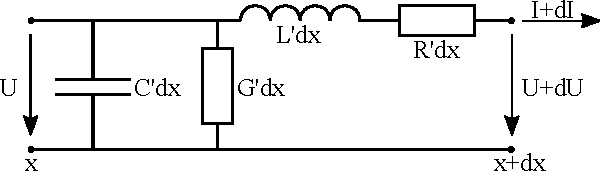
\includegraphics{Schaltungen/Ersatzschaltbild.pdf}
    \caption{Ersatzschaltbild eines homogenen Leitungsstücks infinitesimaler Länge von $x$ bis $x+\de x$.}
    \label{fig:Ersatzschaltbild}
\end{figure}
\paragraph{Induktivität} Ein realer Leiter kann als eine abgewickelte Spule mit einer Windung aufgefasst werden. Es wird im Ersatzschaltbild eine Induktivität $L'\de x$ eingezeichnet, wobei $L' = \frac{L}{\de x}$ den Induktivitätsbelag der Leitung bezeichnet. Der Wert der Induktivität setzt sich aus einem äußeren und inneren Induktivitätsbelag zusammen. Der äußere Induktivitätsbelag ist abhängig vom geometischen Grundaufbau und den magnetischen Eigenschaften der Leitung. Der innere Induktivitätsbelag wird durch magnetische Wechselfelder innerhalb des Leiters verursacht.
\paragraph{Kapazität} Eine Leitung besteht aus mehreren Leiteradern innerhalb des Kabels. Die gegenüberliegenden Flächen der Adern besitzen eine geringe Kapazität $C'\de x$. Der Wert der Kapazität ist abhängig vom geometrischen Aufbau der Leitung und der Dielektrizitätskonstante der Isolierung. Die Kapazität steigt mit geringerem Adernabstand, größerer Leiteroberfläche und höherer Dielektrizitätskonstante an.
\paragraph{Widerstand} Der Widerstand $R' \de x$ einer Leitung beschreibt den den Gleichstromwiderstand einer Ader im Kabel. Mit zunehmender Frequenz nimmt der ohmsche Wechselstromwiderstand der Leitung zu, da durch den Skineffekt die Elektronen an die Leiteroberfläche gedrängt werden und somit der stromdurchflossene Leiterquerschnitt kleiner wird.\\
Der \textbf{Isolationswiderstand} $G'\de x$ beschreibt die Isolations- und dielektrischen Verluste der Leitung. Der Isolationswiderstand ist frequenzabhängig und wird teilweise auch mithilfe des Verlustfaktors $\tan \delta$ angegeben
\begin{align}
  \tan \delta = \frac{G'}{\omega C'}.
\end{align}
\subsubsection{Leitungsgleichungen und Wellenwiderstand}
Zur Beschreibung der Ausbreitung von Strom und Spannung auf einer geraden zweiadrigen Leitung dienen die Leitungsgleichungen. Dabei handelt es sich um ein System gekoppelter partieller Differentialgleichungen, welche unter Verwendung von Knoten- und Maschenregel hergeleitet werden können~\cite{Leitungsgleichungen}
\begin{align}
  \frac{\partial U(x, t)}{\partial x}&=-L'(x) \frac{\partial I(x, t)}{\partial t}-R'(x) I(x, t)\\
  \frac{\partial I(x, t)}{\partial x}&=-G'(x) U(x, t)-C'(x) \frac{\partial U(x, t)}{\partial t}.
\intertext{Unter der Annahme stationärer sinusförmiger Signale ergeben sich folgende Differentialgleichungen der homogenen Leitung}
  \frac{\de U}{\de x} &= -(R' + i\omega L')\cdot I\\
  \frac{\de I}{\de x} &= -(G' + i\omega C')\cdot U
\intertext{Aus diesen Gleichungen lässt sich nun der Wellenwiderstand $Z_L$ bestimmen zu}
  Z_L &= \sqrt{\frac{R'+i\omega L'}{G' + i\omega C'}}\\
  &= \sqrt{\frac{L'}{C'}}\quad \text{verlustfrei.}\label{eqn:Wellenwiderstand}
\end{align}
Bei der Übertragung von Radiowellen wird mit hohen Frequenzen gearbeitet. Deshalb werden die Größen für Isolations- und Widerstandsbelag vernachlässigbar klein, woraus der Leitungswiderstand der verlustlosen Leitung~\eqref{eqn:Wellenwiderstand} resultiert.

\subsubsection{Leistungsanpassung und Reflexionsfaktor}
Im Hochfrequenzbereich muss der \textit{Wellenwiderstand} $Z_L$ der Leitung berücksichtigt werden. Dieser ist eine Kenngröße zur Berechnung des optimalen Abschlusswiderstandes. Dies wird \textit{Widerstandsanpassung} genannt. Hierbei wird gefordert, dass $Z_L = Z_A$ idealerweise gelten muss, um stehende Wellen aufgrund von Reflexionen am Leitungsende zu vermeiden. Dies führt dazu, dass keine Phasenverschiebung zwischen $E$-Feld und $B$-Feld am Leitungsende auftritt und somit keine Leistung reflektiert wird.\\
Wird das Leitungsende kurzgeschlossen, findet eine Reflexion statt und am Leitungsende tritt ein Strommaximum und Spannungsminimum auf. Für eine offene Leitung mit einem theoretisch unendlich großen Abschlusswiderstand wird am Ende die Spannung maximal und der fließende Strom minimal.\\
Zur Beschreibung des Reflexionsanteils wird der \textit{Reflexionsfaktor} $r$ eingeführt als das Verhältnis aus rücklaufender $U_\text{rück}$ und hinlaufender Spannung $U_\text{hin}$
\begin{align}
  r=\frac{U_{\text{Rück}}}{U_{\text{Hin}}}=\frac{Z_{A}-Z_{L}}{Z_{A}+Z_{L}} \Rightarrow-1 \leq r \leq 1.
\end{align}
Bei der Verwendung von Sinussignalen bilden sich stehende Wellen durch Interferenz von hinlaufender und refelektiereter Welle aus. Alternativ zum Reflexionsfaktor wird das Stehwellenverhältnis \text{VSWR} (voltage standing wave ratio) definiert
\begin{align}
  VSWR=\frac{U_{\max }}{U_{\min }}= \frac{U_\text{Hin}+U_\text{Rück}}{U_\text{Hin}-U_\text{Rück}}\frac{1+|r|}{1-|r|} \Rightarrow 1 \leq VSWR<\infty.
\end{align}
Es gibt das Verhältnis von Spannungsmaximum und -minimum der stehenden Welle innerhalb des Leiters an.

\subsubsection{Leitungsarten}
Da zur Übertragung hoher Frequenzen $\nu > \SI{1}{\mega\hertz}$ gewöhnliche Laborkabel mit Bananenstecker ungeeignet sind, werden alternative Leitungsarten eingesetzt. Bei den im Praktikum verwendeten Kabeln handelt es sich um Koaxialleitungen, welche selbstabschirmend sind und einen Wellenwiderstand von $Z_L = \SI{50}{\ohm}$ (in der Antennentechnik $Z_L = \SI{75}{\ohm}$) besitzen. Koaxialkabel sind die am meisten verwendete Leitungsart.\\
Die Lecherleitung bzw. Zweidrahtleitung ist die ursprüngliche Leitungsart zu Übertragung hochgfrequenter Signale. Aufgrund der kostengünstigen Herstellung werden sie häufig in der Computertechnik eingesetzt.\\
In der Telekommunikations- und Computertechnik werden ebenso \textit{Twisted-Pair}-Kabel benutzt, deren Adernpaare miteinander verdrillt sind. Der bekannteste Anwendungsbereich sind Netzwerkkabel, wo vier Adernpaare zu einem Kabel zusammengefasst sind.
Für die Übertragung höhrerer Frequenzen ab $\SI{6}{\giga\hertz}$ sollten Hohlleiter verwendet werden, da diese verlustärmer sind als Koaxialkabel. Allerdings sind Hohlleiter erst ab einer kritischen Frequenz funktionsfähig.

\subsection{Modulation}
Als Modulation wird das Aufprägen einer Information auf eine Trägerschwingung bezeichnet. Dabei wird das zu übertragene Nutzsignal in einen definierten höheren Frequenzbereich verschoben. Dies wird benötigt, weil der direkte Übertragungsweg des Signals durch ein Medium wie z.\,B. Schall häufig nicht über lange Strecken möglich ist. Im Allgemeinen erfolgt die Signalübertragung über einen Kanal wie Luft oder Kabel. Im Kanal tritt eine frequenzabhängige Dämpfung auf, weshalb das Signal auf eine Frequenz innerhalb eines dämpfungsarmen Frequenzfensters moduliert wird. Für das Nutzsignal und den Träger lassen sich folgende Formeln aufstellen.
\begin{align}
    U_\text{Nutz}(t) &= U_\text{N}\cdot\cos(\omega_\text{N}t) & \text{Spannung Nutzfrequenz}\\
    U_\text{Träger}(t) &= U_\text{T}\cdot\cos(\omega_\text{T}t) & \text{Spannung Trägerfrequenz}
\end{align}
Der Träger wird benötigt, um die Information des Nutzsignals durch spätere Demodulation wieder zu erhalten.\\
Die Mischung zweier Signale wird technisch auf gleiche Weise realisiert wie die Modulation. Bei der Mischung wird nur eine der entstehenden Frequenzen weiter benutzt, während bei der Modulation mehrere Mischprodukte weiter verwendet werden.
\subsubsection{Amplitudenmodulation}
Bei der Amplitudenmodulation wird das Signal in der Amplitude der Trägerschwingung kodiert. Die Amplitude des modulierten Signals ändert sich mit der Frequenz des Nutzsignals, während die Schwingungsfrequenz durch den Träger vorgegeben wird. Es lassen sich zwei verschiedene Verfahren unterscheiden.
\paragraph{Additive Amplitudenmodulation}
Hierbei handelt es sich um die am einfachsten realisierbare Variante. Die zu modulierenden Signale werden überlagert und anschließend an einer Kennlinie (Diode oder Transistor) mit exponentiellen Verlauf verzerrt. Dabei entstehen neue Frequenzkomponenten.
\begin{align}
  U_\text{AM}(t) = U_\text{T}\cos(\omega_\text{T}t) + U_\text{N}\cos(\omega_\text{N}t)\cdot\cos(\omega_\text{T}t)\label{eqn:AM_additiv}
\end{align}
Neben der Trägerfrequenz $\omega_\text{T}$ entstehen im amplitudenmodulierten Signal zwei weitere Frequenzen. Diese Schwebungsfrequenzen $\omega_\text{T} \pm \omega_\text{N}$ werden als Seitenbänder bezeichnet.
\begin{align}
  U_\text{oberes Seitenband}\cos(\omega_\text{T} + \omega_\text{N})\\
  U_\text{unteres Seitenband}\cos(\omega_\text{T} - \omega_\text{N})
\end{align}
Üblicherweise wird die Trägerfrequenz $\omega_\text{T}$ so gewählt, dass sie viel größer als die Signalfrequenz ist, $\omega_\text{S} \ll \omega_\text{T}$, weshalb alle auftretenden Frequenzen im Größenbereich der Trägerfrequenz liegen.\\
Eine weitere charakteristische Größe stellt der Modulationsgrad $M$ dar. Dieser ist definiert als Verhältnis der Hüllkurvenamplitude zur Trägeramplitude und berechnet sich folgendermaßen
\begin{align}
  M = \frac{U_N}{U_T} = \frac{\text{max}-\text{min}}{\text{max}+\text{min}},\label{eqn:Modulationsgrad}
\end{align}
wobei die beiden Größen in Abbildung~\ref{fig:Amplitudenmodulation} eingezeichnet sind.
\begin{figure}[htp]
    \centering
        \begin{center}
	\newcommand\maxt{2} % in [s]
	\newcommand\fTraeger{20} % in [Hz]
	\newcommand\fSignal{1.5} % in [Hz]
	\newcommand\Modulationstiefe{50} % in Prozent

	\begin{tikzpicture}[trim axis left, trim axis right]
  	\begin{axis}[
    	clip=false,
    	width=0.9\textwidth, height=0.3\textwidth,
    	xlabel={$t$ [\si{\second}]},
    	ylabel={Amplitude [\si{\volt}]},
    	xmin=0, xmax=\maxt,
    	xtick distance=0.5,
    	minor x tick num=4,
    	ytick distance=1,
    	minor y tick num=4,
    	legend style={cells={anchor=west}, legend pos=outer north east,},
    	]
      \addplot [domain=0:{\maxt}, samples=500, smooth, mark=none, thick, color=blue, solid] {cos(deg(2*pi*\fTraeger*x))*(1 + (\Modulationstiefe/100)*(cos(deg(2*pi*(\fSignal)*x))))};
      \addplot [domain=0:{\maxt}, samples=100, smooth, mark=none, thick, color=black, densely dotted, forget plot] {+1*(\Modulationstiefe/100)*cos(deg(2*pi*\fSignal*x)) + 1};
      \addplot [domain=0:{\maxt}, samples=100, smooth, mark=none, thick, color=black, densely dotted, forget plot] {-1*(\Modulationstiefe/100)*cos(deg(2*pi*\fSignal*x)) - 1};
    	\draw [thick, black, stealth-] ({0.5/\fSignal},{+1-(\Modulationstiefe/100)}) -- ({0.5/\fSignal},{+1-(\Modulationstiefe/100) + 0.4});
    	\draw [thick, black, stealth-] ({0.5/\fSignal},{-1+(\Modulationstiefe/100)}) -- ({0.5/\fSignal},{-1+(\Modulationstiefe/100) - 0.4}) node[below,fill=gray!50!white,rectangle,rounded corners=3pt]{min};
    	\draw [thick, black, stealth-] ({1/\fSignal},{+1+(\Modulationstiefe/100)}) -- ({1/\fSignal},{0});
    	\draw [thick, black, stealth-] ({1/\fSignal},{-1-(\Modulationstiefe/100)}) -- ({1/\fSignal},{0});
    	\path ({1/\fSignal},{+1+(\Modulationstiefe/100)}) -- node[fill=gray!50!white,rectangle,rounded corners=3pt]{max} ({1/\fSignal},{-1-(\Modulationstiefe/100)});
  	\end{axis}
	\end{tikzpicture}
\end{center}

    \caption{Amplitudenmodulation eines Signals $\nu_\text{N} = \SI{1.5}{\hertz}$ mit der Trägerfrequenz $\nu_\text{T} = \SI{20}{\hertz}$ mit Modulationstiefe $M = \SI{50}{\percent}$ (eigene Abbildung).}
    \label{fig:Amplitudenmodulation}
\end{figure}\\
Bei einem Modulationsgrad von $\SI{100}{\percent}$ fällt die Amplitude des modulierten Signals auf $\SI{0}{\volt}$ ab.
\paragraph{Multiplikative Amplitudenmodulation}
Diese Modulationsvariante wird in der Praxis häufiger eingesetzt und kann mit Diodenringmodulatoren realisiert werden. Dabei werden die beiden Schwingungen direkt miteinander multipliziert
\begin{align}
    U_\text{AM} = U_\text{N} \cos(\omega_\text{N}t)\cdot U_\text{T} \cos(\omega_\text{T}t).\label{eqn:AM1_multiplikativ}
\end{align}
Der Unterschied zur additiven Variante besteht darin, dass die Trägerfrequenz nicht mit erzeugt wird und unerwünschte Nebenfrequenzen unterdrückt werden. Das Minimum im Zeitsignal zeigt einen Phasensprung.

\subsubsection{Frequenzmodulation}
Bei der Frequenzmodulation wird die Amplitude des modulierten Signals konstant gehalten und durch das Trägersignal charakterisiert. Die Information des Nutzsignals wird durch die sich ändernde Frequenz übertragen. Es ergibt sich für die Frequenzmodulation folgende Formel
\begin{align}
  U_\text{FM}(t) = U_\text{T} \cos\left[\omega_\text{T} \frac{\Delta \omega}{\omega_\text{S}}\cdot \sin(\omega_\text{S}t)\right].
\end{align}
Es wird ein symmetrisch zur Trägerfrequenz $\omega_\text{T}$ liegender Frequenzbereich durchlaufen. Die maximale Abweichung von der Trägerfrequenz wird mit $\Delta \omega = (\omega_\text{max}-\omega_\text{min})/2$ bezeichnet. Für die nachfolgende Betrachtung ist es sinnvoll, den Modulationsindex $\eta$ als das Verhältnis aus Frequenzhub $\Delta \omega$ und Nutzfrequenz $\omega_\text{N}$ zu definieren
\begin{align}
  \eta = \frac{\Delta \omega}{\omega_\text{N}} = \frac{\text{Frequenzhub}}{\text{Signalfrequenz}}.
\end{align}
Abbildung~\ref{fig:FM} zeigt den Zeitverlauf eines frequenzmodulierten Signals mit Frequenzhub $\Delta f = \SI{5}{\hertz}$ und Modulationsindex $\eta = 3,33$.
\begin{figure}[htp]
    \centering
        \begin{center}
	\newcommand\maxt{2} % in [s]
	\newcommand\fSignal{2} % in [Hz]
	\newcommand\fTraeger{20} % in [Hz]
	\newcommand\Frequenzhub{5} % in [Hz]
	\pgfmathparse{\Frequenzhub/\fSignal}
	\xdef\Modulationsindex{\pgfmathresult}
	\pgfmathparse{1/\fSignal}
	\xdef\Periodendauer{\pgfmathresult}
	\begin{tikzpicture}[trim axis left, trim axis right]
	\begin{axis}[
	width=0.78\textwidth, height=0.3\textwidth,
	xlabel={Zeit $t$ in \si{\second}},
	ylabel={Amplitude in \si{\volt}},
	xmin=0, xmax=\maxt,
	xtick distance=0.5,
	minor x tick num=4,
	ymin=-2.2, ymax=+2.2,
	ytick distance=1,
	minor y tick num=4,
	legend style={cells={anchor=west}, legend pos=outer north east,},
	]
	\draw [gray] (0,+1) -- (\maxt,+1);
	\draw [gray] (0,-1) -- (\maxt,-1);
	\addplot [domain=0:{\maxt}, samples=1000, smooth, mark=none, thick, color=blue, solid] {cos(deg(2*pi*\fTraeger*x)) + 1};
	\addlegendentry{$U_{\text{T}} (t)$}
	\addplot [domain=0:{\maxt}, samples=100, smooth, mark=none, thick, color=black, solid] {cos(deg(2*pi*\fSignal*x)) + 1};
	\addlegendentry{$U_{\text{N}} (t)$}
	\addplot [domain=0:{\maxt}, samples=1000, smooth, mark=none, thick, color=orange, solid] {cos(deg(2*pi*\fTraeger*x + \Frequenzhub*sin(deg(2*pi*\fSignal*x)))) - 1};
	\addlegendentry{$U_{\text{FM}} (t)$}
	\end{axis}
	\end{tikzpicture}
\end{center}

    \caption{Frequenzmodulation eines sinusförmigen Signals der Frequenz $\nu_\text{S} = \SI{2}{\hertz}$ auf eine Trägerschwingung der Frequenz $\nu_\text{T} = \SI{20}{\hertz}$}
    \label{fig:FM}
\end{figure}
\FloatBarrier
\noindent
Die Auswirkung des Modulationsindex auf das Frequenzspektrum des modulierten Signals lässt sich mathematisch mithilfe von Bessel-Funktionen ausdrücken.
\begin{align}
    J_m(\eta) &= \frac{1}{\pi}\int_0^\pi \cos(\eta\sin \vartheta - m\vartheta)\; \text{d}\vartheta\\
    J_{m+1} (\eta) &= \frac{2m}{\eta} \cdot J_m(\eta) - J_{m-1}(\eta).
\end{align}
\begin{figure}[htp]
    \centering
    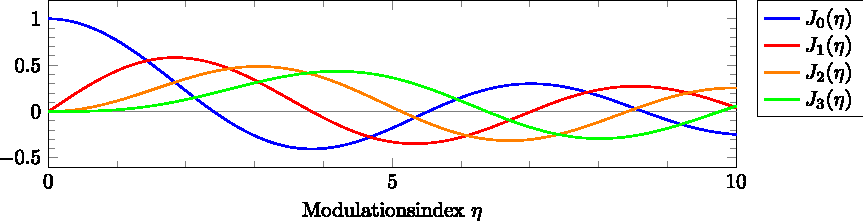
\includegraphics[width=0.9\textwidth]{Schaltungen/Besselfunktion.pdf}
    \caption{Verlauf der Besselfunktionen. Die Amplitude der Besselfunktion $J_i$ gibt den Anteil der Seitenbänder $\omega_\text{T}\pm\omega_{i\cdot\text{N}}$ im Frequenzspektrum an.}
    \label{fig:Besselfunktionen}
\end{figure}
Zum Herausfiltern von bestimmten Frequenzanteilen aus dem Signal, muss ein Modulationsindex $\eta$ gewählt werden, für den die entsprechende Besselfunktion eine Nullstelle aufweist.
\newpage
\subsection{Demodulation}
Bei der Demodulation wird aus dem übertragenen modulierten Signal wieder das ursprüngliche Nutzsignal zurückgewonnen. Für die Demodulation wird das Signal zunächst mit einer Diode gleichgerichtet, um die untere Halbwelle des Signals zu entfernen. Im zweiten Schritt wird das Signal mithilfe eines Kondensators geglättet, der aufgrund seiner im Vergleich zur Trägerfrequenz großen Zeitkonstante einen Spannungsverlauf erzeugt, der dem Verlauf der Hüllkurve ähnelt. Der Kondensator wirkt also eine Art Tiefpass. Am Ende ergibt sich die Hüllkurve, welche bis auf einem konstanten Gleichstromanteil dem ursprünglichen Signal entspricht. Der im Versuch verwendete Modulator lässt sich durch das Schaltbild in Abbildung~\ref{fig:Demodulator} veranschaulichen.
\begin{figure}[htp]
    \centering
    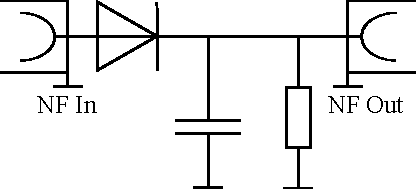
\includegraphics[width=0.5\textwidth]{Schaltungen/Demodulator.pdf}
    \caption{Schaltbild des im Versuch verwendeten Demodulators.}
    \label{fig:Demodulator}
\end{figure}\\
Durch einen weiteren, in Reihe geschalteten Kondensator lässt sich zusätzlich noch der Gleichspannungsanteil des demodulierten Signals entfernen.

\subsection{Elektromagnetische Wellen im freien Raum}
Die Propagation von elektromagnetischen Wellen im freien Raum bildet die Grundlage aller Funkanwendungen und ist im Alltag unabdingbar. Zur Nutzung der elektromagnetischen Wellen im freien Raum müssen diese über Antennen abgestrahlt und empfangen werden. Dabei muss eine Anpassung an den Wellenwiderstand des freien Raumes durchgeführt werden. Dieser gibt das Verhältnis der Beträge von elektrischem und magnetischem Feld an
\begin{align}
  Z_0 = \frac{|\bm{E}|}{|\bm{H}|} = \sqrt{\frac{\mu_0}{\varepsilon_0}} \approx \SI{377}{\ohm}.
\end{align}\\
Die für die Signalübertragung verwendeten Antennen bilden einen schwingenden Dipol aus einem Kondensator und einer Spule. Technisch wird eine Antenne durch das Aufklappen eines Dipols realisiert, welcher elektromagnetische Wellen in alle Richtungen (mit Ausnahme der Bewegungsrichtung der Elektronen in der Antenne) abstrahlt.
\begin{figure}[htp]
    \centering
    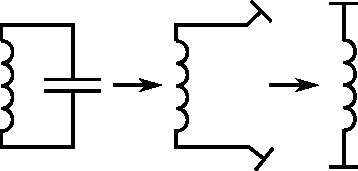
\includegraphics{Schaltungen/offenerSchwingkreis.pdf}
    \caption{Prinzipielle Konstruktion einer Antenne als ein offener Schwingkreis.}
    \label{fig:Schwingkreis}
\end{figure}\\
Die durch die Abstrahlung elektromagnetischer Wellen entnommene Energie muss dem Schwingkreis durch einen Generator wieder zugeführt werden.
\paragraph{Antennen}
Prinzipiell gibt es zwei Möglichkeiten, eine Antenne zu konstruieren. Es wird zwischen Halbwellendipolen und Viertelwellendipolen unterschieden. Bei beiden Konstruktionsarten wird das Ausbilden stehender Wellen im Leiter explizit genutzt und die Länge der Antenne entsprechend eingestellt. Wie die Bezeichnung bereits impliziert, wird die Länge der Antenne für eine bestimmte Empfangs- oder Abstrahlungsfrequenz so eingestellt, dass ihre Länge genau der Hälfte, bzw. dem Viertel der Wellenlänge entspricht.\\
Bei einer $\lambda/2$-Antenne gibt es zwei Enden mit einem offenen Abschluss, in der Mitte (Fußpunkt) wird das Signal abgeführt. Durch den hohen Abschlusswiderstand tritt am Antennenende ein Spannungsmaximum auf, wodurch am Fußpunkt bei $\lambda/4$ ein Spannungsminimum und Strommaximum entsteht.\\
Bei der $\lambda/4$-Antenne befindet sich der Fußpunkt am Antennenende, am offenen Ende liegt wieder ein Spannungsmaximum vor, woraus ein Minimum am Fußpunkt resultiert. Es ist jedoch wichtig, darauf zu achten, dass der materialbedingte Verkürzungsfaktor der Antenne bei der Längeneinstellung beachtet wird.\\
Für einen unendlich dünnen Halbwellendipol gilt für die Antenenimpendanz
\begin{align}
  Z_\text{Ant} = R_\text{Ant} + i X_\text{Ant} = (73,13 + i\cdot 42,54)\si{\ohm}
\end{align}
Damit eine reelle Antennenimpendanz erzielt wird, um die Antenne in Resonanz betreiben zu können, muss der induktive Anteil verschwinden. Dies wird durch Verkürzen der Antenne erreicht und es ergibt sich ein Verkürzungsfaktor von
\begin{align}
  K_\text{Ant} = 0,96.
\end{align}
% *********************************************
% ***** KAPITEL 3 *****************************
% *********************************************
\section{Versuchsdurchführung} \label{sec:Versuchsdurchführung}
\subsection{Elektromagnetische Wellen auf Leitungen}
\subsubsection{Verhalten von Sinussignalen}
Die Frequenzgänge im Bereich \SI{1}{\mega\hertz} bis \SI{100}{\kilo\hertz} verschiedener Kabelanordnungen werden gemessen und graphisch dargestellt. Dazu wird ein HF Generator mit Ausgang \SI{50}{\ohm} und nachgeschaltetem Teiler 10:1 mit Hilfe der jeweiligen Kabelart mit einem Scope verbunden, an welchem jeweils der Eingangswiderstand zwischen \SI{50}{\ohm} und \SI{1}{\mega\ohm} variiert wird. An diesem wird auch die jeweilige zur Frequenz gehörenden Spannung abgelesen. Dabei werden
\begin{itemize}
  \item Laborkabel (ca. \SI{2}{\metre} Länge)
  \begin{itemize}
    \item Scope Eingangwiderstand \SI{1}{\mega\ohm}
    \item Scope Eingangswiderstand \SI{50}{\ohm}
  \end{itemize}
  \item{Koaxialkabel (ca. \SI{2}{\metre} Länge)}
  \begin{itemize}
    \item Skope Eingangswiderstand \SI{1}{\mega\ohm}
    \item Skope Eingangwiderstand \SI{50}{\ohm}
  \end{itemize}
  \item Koaxialkabel mit über T-Stück zusätzlich angeschlossenem Stichkabel (Länge: \SI{2,48}{\metre}) bei einem Skope Eingangwiderstand von \SI{50}{\ohm}
  \begin{itemize}
    \item Abschluss des Stichkabels: offen
    \item Abschluss des Stichkabels: Kurzschluss (realisiert durch Kurzschlussstecker)
    \item Abschluss des Stichkabels: Wellenwiderstand (realisiert durch \SI{50}{\ohm}- Stecker)
  \end{itemize}
  vermessen.
\end{itemize}

Anschließend werden Verkürzungsfaktor, Ausbreitungsgeschwindigkeit und Permitivität für das Koaxialkabel mit dem vorhergehenden Messaufbau bestimmt.

\subsubsection{Verhalten von Rechtecksignalen}
Mit dem Funktionsgenerator Agilent 33220A wird ein Rechtecksignal (\SI{50}{\nano\second}, \SI{100}{\kilo\hertz} erzeugt. Dieser ist über ein ca. \SI{2}{\metre} langes Koaxialkabel mit dem Scope verbunden, auf welchem das Signal beobachtet wird. Dabei wird als Eingangswiderstand \SI{50}{\ohm} bzw. \SI{1}{\mega\ohm} gewählt.\\
Anschließend wird ein \SI{25}{\metre} langes Koaxialkabel mit einem T-Stück als Stichkabel an das den Frequenzgenerator und Scope verbindende Kabel angeschlossen. Der Scope hat einen Eingangwiderstand von \SI{50}{\ohm}. Hier werden die Impulsformen am Anfang des Kabels bei folgenden Abschlusswiderständen am Ende des Kabels beobachtet:
\begin{itemize}
  \item $Z_A = \infty$ (offenes Leitungsende)
  \item $Z_A = \SI{0}{\ohm}$ (Kurzschlussstecker)
  \item $Z_A = Z_L$ (Stecker mit Wellenwiderstand \SI{50}{\ohm})

\end{itemize}

Anschließend wird für $Z_A=Z_L$ und $Z_A = \infty$ das Signal zusätzlich am Ende des Stichkabels beobachtet. Dazu wird das Ende des Stichkabels an den 2. Eingang des Scopes angeschlossen und der Eingangswiderstand dieses Eingangs einmal auf \SI{50}{\ohm} (entspricht $Z_A = Z_L$) und einmal auf \SI{1}{\mega\ohm} (entspricht $Z_A = \infty)$ eingestellt. \\

Außerdem wird der gleiche Rechteckpuls mit Laborkabeln übertragen. Auch hierbei wird der Eingangswiederstand einmal auf \SI{50}{\ohm} und einmal auf \SI{1}{\mega\ohm} eingestellt. \\

Die Ausbreitungsgeschwindigkeit, der Verkürzungfaktor und die Permitivität werden bestimmt, indem ein \SI{25}{\metre} langes als Stichkabel auf das den Frequenzgenerator und den Scope verbindende Kabel angebracht und ein Rechtecksignal durch die Leitung geschickt wird. Aus der Verschiebung zweier Flanken errechnet sich die Ausbreitungsgeschwindigkeit und daraus anschließend der Verkürzungsfaktor und die Permitivität. Alternativ werden alle drei Größen auch bestimmt, indem das Stichkabel mit dem Scope im zweiten Eingang mit Eingangwiderstand \SI{50}{\ohm} verbunden wird und die Verschiebung des durchlaufenden mit dem am Ende des Stichkabels ankommenden Pulses für Berechnungen genutzt wird.

\subsubsection{Wellenwiderstandsbestimmung mit Rechteckimpulsen}\label{subsec:BestimmungZL}
Frequenzgenerator und Scope werden über ein kurzer Koaxialkabel miteinander verbunden. Ein \SI{50}{\metre} langes Koaxialkabel wird als Stichkabel über ein T-Stück angeschlossen. Das Ende dieses Stichkabels wird mit einem veränderbaren Widerstand (Potentiometer) abgeschlossen. Am Scope werden die Reflexionen der Impulse am Anfang der Leitung in Abhängigkeit vom Widerstand beobachtet und diejenige EInstellung von R bestimmt, sodass die Reflexionen minimal sind. Dieser eingestellte Widerstand wird mit Hilfe eines Multimeters vermessen.

\subsubsection{Wellenwiderstandsbestimmung durch L und C Messung}
Für diese Messung wird eine LC-Messbrücke verwendet. Für die Messung der Kapazität wird das Leitungsende offen gelassen, wird die Induktivität gemessen, so wird ein Kurzschlussstecker als Abschlusswiderstand des Kabels genutzt.

\subsection{Modulation}
Zunächst werden mithilfe eines LabView Programms die Addition von Signalen, sowie additive und multiplikative Amplitudenmodulation simuliert und ausgewertet.\\
Anschließend erfolgt eine additive Amplitudenmodulation mithilfe eines Modulators (siehe Abbildung~\ref{fig:AM_Modulator}).\\
Das modulierte Signal wird am Scope und am Spektrumsanalysator dargestellt und ausgewertet. Die Messung wird für verschiedene Modulationsgrade unter Variation der Signalspannung wiederholt.\\
Schließlich wird eine Demodulation eines amplitudenmodulierten Signals der Frequenz $\nu_\text{N} = \SI{500}{\hertz}$ durchgeführt und mithilfe des Scopes ausgewertet. Für das demodulierte Signal wird eine Frequenzbestimmung vorgenommen.

\subsection{Elektromagnetische Wellen im freien Raum}
Es wird eine $\lambda/2$ Antenne auf eine Frequenz von \SI{200}{\mega\hertz} eingestellt. Dazu wird eine Reflektometer genutzt um bei Verändern der Länge der Antenne, die jeweilige Frequenz zu finden, bei der die rücklaufende Spannung ein Minima aufweist. Das Reflektometer wird dazu zwischen Spannunsgquelle und Antenne geschaltet und die rücklaufende Spannung am entsprechenden Ast abgenommen und am Scope dargestellt. Es wird die Länge eingestellt, sodass sich das Minimum der Spannung bei der gegebenen Frequenz befindet. Anschließend werden Stehwellenverhältnis, Reflektionsfaktor und Verkürzungsfaktor bestimmt und eine zweite Antenne mit den gleichen Maßen eingestellt. \\
Die Sendeantenne wird mit einem Generator verbunden, die Empfangsantenne mit dem Scope bzw dem Spektrumsanalysator. Ein Signal mit \SI{200}{\mega\hertz} und \SI{1}{\volt}-Effektivspannung wird genutzt. Das Signal wird übertragen und empfangen und die jeweiligen Leistungen bei unterschiedlichen Ausrichtungen der Empfangsantenne werden bestimmt. \\
Anschließend wird mit einem Modulator eine additive Amplitudenmodulation durchgeführt. Dazu wird eine Nutzfrequenz von \SI{500}{\hertz} bei einer Spannung von \SI{0,4}{\volt} und eine Trägerfrequenz von \SI{200}{\mega\hertz} bei einer Spannung von \SI{1}{\volt} verwendet. Das modulierte Signal wird auf die Sendeantenne gegeben und abgestrahlt und von der Empfangsantenne empfangen. Letztere ist mit einem Demodulator verbunden, von dem aus das Signal dann am Scope dargestellt wird. Die Ausrichtung der Empfangsantenne wird variiert und das Ergebnis am Scope beobachtet. Anschließend wird das Signal hörbar gemacht, indem der Ausgang des Demodulators mit einem Lautsprecher verbunden wird.
% *********************************************
% ***** KAPITEL 4 *****************************
% *********************************************
\newpage
\section{Ergebnisse und Diskussion}
\subsection{Elektromagnetische Wellen auf Leitungen}
\subsubsection{Verhalten von Sinussignalen}
Die im Bereich \SI{1}{\mega\hertz} bis \SI{100}{\kilo\hertz} gemessenen Frequenzgänge verschiedener Kabelanorndungen sind im Folgenden graphisch dargestellt.
\paragraph{Laborkabel (Länge ca. \SI{2}{\metre})}
Während der Messung mit den Laborkabeln fällt auf, dass sich durch kleine Veränderungen der Anordnung der Kabel bzw. Bewegung der Kabel wie zum Beispiel durch Wackeln der Wert der angezeigten Spannung bei gleicher Frequenz ändert. Eine Kabelbewegung führt also zu einem anderen Frequenzgang bzw. Spannungsverlauf. Trotz Verwendung des gleichen Kabels ist es nicht möglich, einen identischen Frequenzgang bei einer späteren Messung zu erhalten. Der in Abbildung~\ref{fig:Frequenzgang_Laborkabel} zeigt das Ergebnis einer exemplarischen Messung.
\begin{figure}[htp]
    \centering
        \vspace{-0.5cm}
        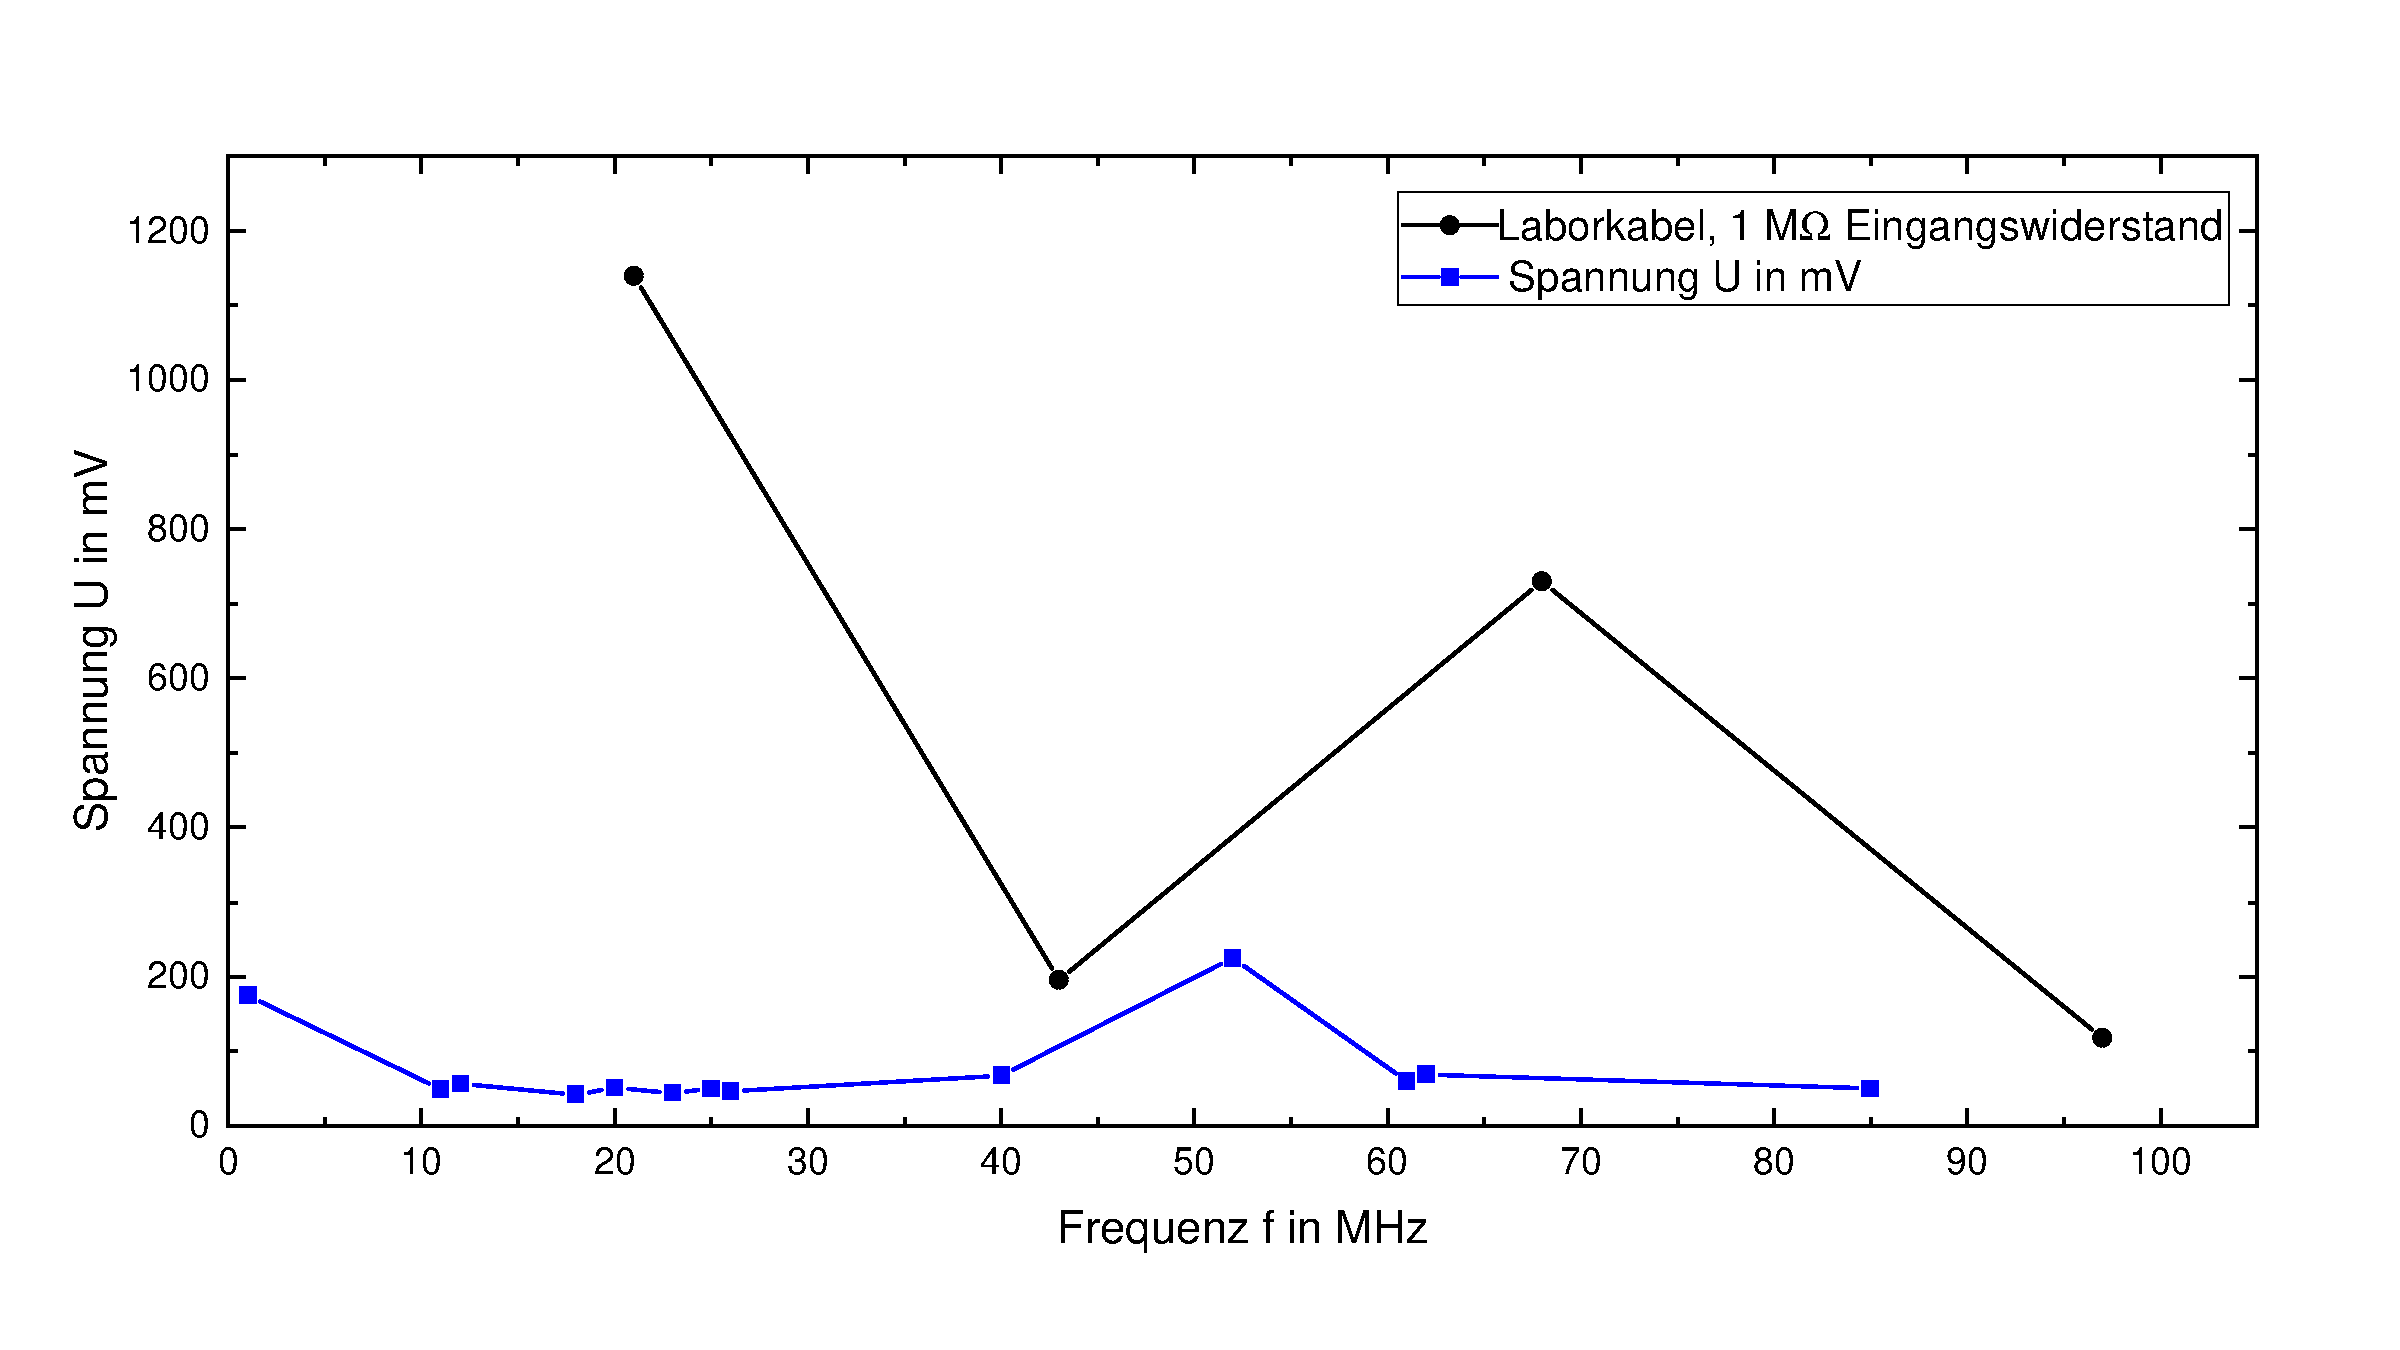
\includegraphics[width=0.9\textwidth]{Bilder/Laborkabel_50_1MOhm.pdf}
        \vspace{-0.25cm}
    \caption{Frequenzgang von Laborkabeln als Verbindung zwischen Generator und Scope (Eingangswiderstand \SI{50}{\ohm} und \SI{1}{\mega\ohm}) }
    \label{fig:Frequenzgang_Laborkabel}
\end{figure}\\
Im Allgemeinen weisen die Kabel sowohl bei \SI{50}{\ohm}, als auch bei \SI{1}{\mega\ohm} Eingangwiderstand des Scopes einen chaotischen Frequenzgang auf (bei \SI{1}{\mega\ohm} wurden nur globale Maxima und Minima vermessen, aber auch zwischen diesen Peaks wurden immer wieder lokale Minima und Maxima festgestellt). Bei \SI{1}{\mega\ohm} kommt es dazu, dass die Spannung bei bestimmten Frequenzen höher wird, als die, die ursprünglich herein gegeben wurde. Das Kabel wirkt hierbei als Transformator.
Auch bei Verwendung eines \SI{50}{\ohm} Eingangwiderstand des Scopes schwankt die Spannung bei Erhöhung der Frequenz merklich hin und her. Innerhalb kleiner Frequenzbereiche zeigen sich immer wieder lokale Minima und Maxima.\\
Wegen der bereits erklärten Abhängigkeit eines Spannungswertes bei gleicher Frequenz von der Anordnung der Kabel sowie des chaotischen Verlaufs auch bei \SI{50}{\ohm} des sind die Laborkabel als ungeeignet für Messungen in der Hochfrequenztechnik einzustufen.

\paragraph{Koaxialkabel (Länge ca. \SI{2}{\metre})}
Auch bei den Koaxialkabeln wird bei einem Eingangswiderstand des Scopes von \SI{1}{\mega\ohm} bei Frequenzen von ungefähr \SI{20}{\mega\hertz} und \SI{70}{\mega\hertz} Maxima festgestellt, an denen Spannungen gemessen werden, die über der Spannung liegt, die eingegeben wurde. Diese Maxima treten periodisch auf, wie in Abbildung~\ref{fig:Frequenzverlauf_Koaxialkabel} dargestellt wird.
\begin{figure}[htp]
    \centering
    \vspace{-0.5cm}
        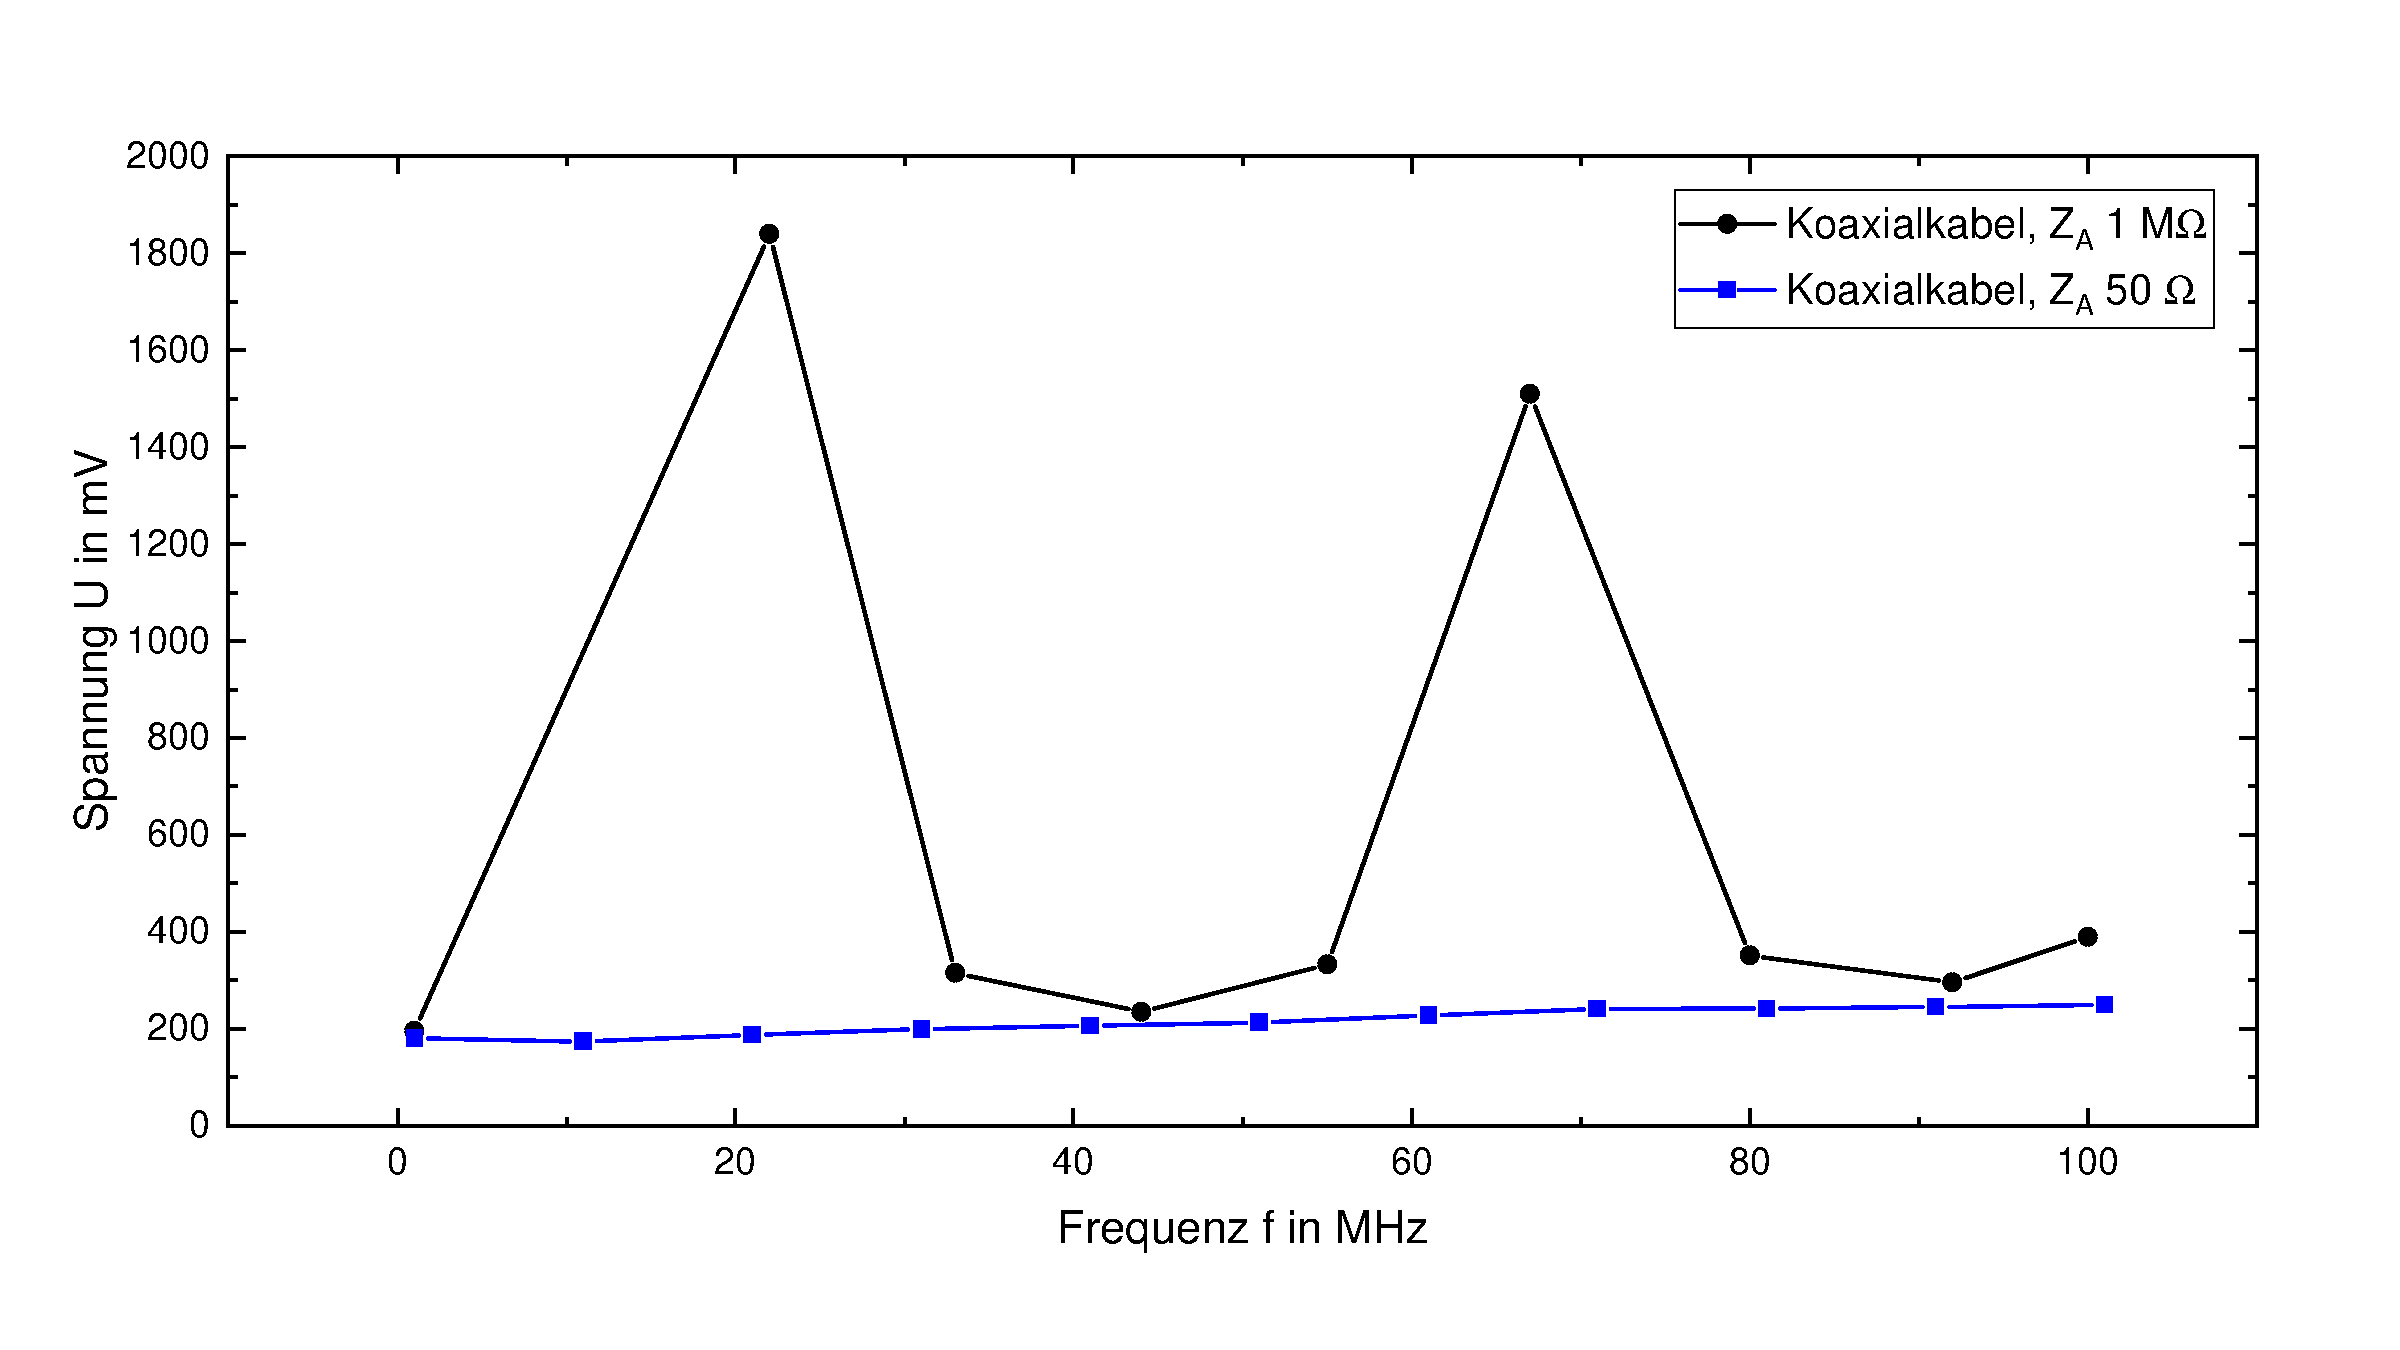
\includegraphics[width=0.9\textwidth]{Bilder/Koaxialkabel_50_1MOhm.pdf}
        \vspace{-0.25cm}
    \caption{Frequenzgang von Koaxialkabel als Verbindung zwischen Generator und Scope (Eingangswiderstand \SI{50}{\ohm} und \SI{1}{\mega\ohm})}
    \label{fig:Frequenzverlauf_Koaxialkabel}
\end{figure}
Bei einem Eingangwiderstand des Scopes von \SI{1}{\mega\ohm} liegt eine falsche Anpassung vor, welche zu Reflexion und zu stehenden Wellen führt. In den genannten Fällen kommt es so zu einer Spannungsverstärkung. Diese Eigenschaft eröffnet die Möglichkeit der Verwendung der Koaxialkabel bei diesem Frequenzen als Transformator und bietet damit eine Alternative zum Transformieren mit einem Schwingkreis.
Ebenso periodisch treten auch Minima auf. Hier kommt es aufgrund der Reflexionen zu Auslöschungen und damit zu niedrigeren gemessenen Spannungen. Diese eignen sich in der Praxis besser zum Auswerten. Ein Spannungsmaxima ist nicht so gut messbar, da das Messgerät in diesem Fall sehr hochohmig sein müsste. Dies ist praktisch schwer zu realisieren, weshalb es zu einer Verfälschung der Spannung bei Messung von Maxima kommt.\\
Bei einem Eingangswiderstand von \SI{50}{\ohm} wird Anpassung erreicht. Die komplette Energie der Welle wird in den Abschlusswiderstand aufgenommen, es kommt nicht zu Reflexionen und damit zu einer konstanten Spannung über alle Frequenzen.

\paragraph{Koaxialkabel mit Stichkabel}
Es wurde zusätzlich über ein T-Stück ein Stichkabel der Länge $L=\SI{2,48}{\metre}$ angeschlossen. Bei der Analyse der Frequenzgänge bei Verwendung eines Stichkabels jeweils mit offenem Ende, Kurzschlusstecker oder \SI{50}{\ohm} - Steckers fällt auf, dass in der Nähe der Frequenzen, wo die Spannung bei offenem Ende des Stichkabels, und damit nährungsweise unendlichem Abschlusswiderstand $Z_A$, ein Maximum zeigt, bei Verwendung eines Kurzschlussteckers, und damit ungefähr Abschlusswiderstand \SI{0}{\ohm}, am Ende des Stichkabels ein Minimum aufweist (siehe Abbildung~\ref{fig:Frequenzgang_Koaxialkabel_Stichkabel}).
\begin{figure}[htp]
    \centering
        \vspace{-0.5cm}
        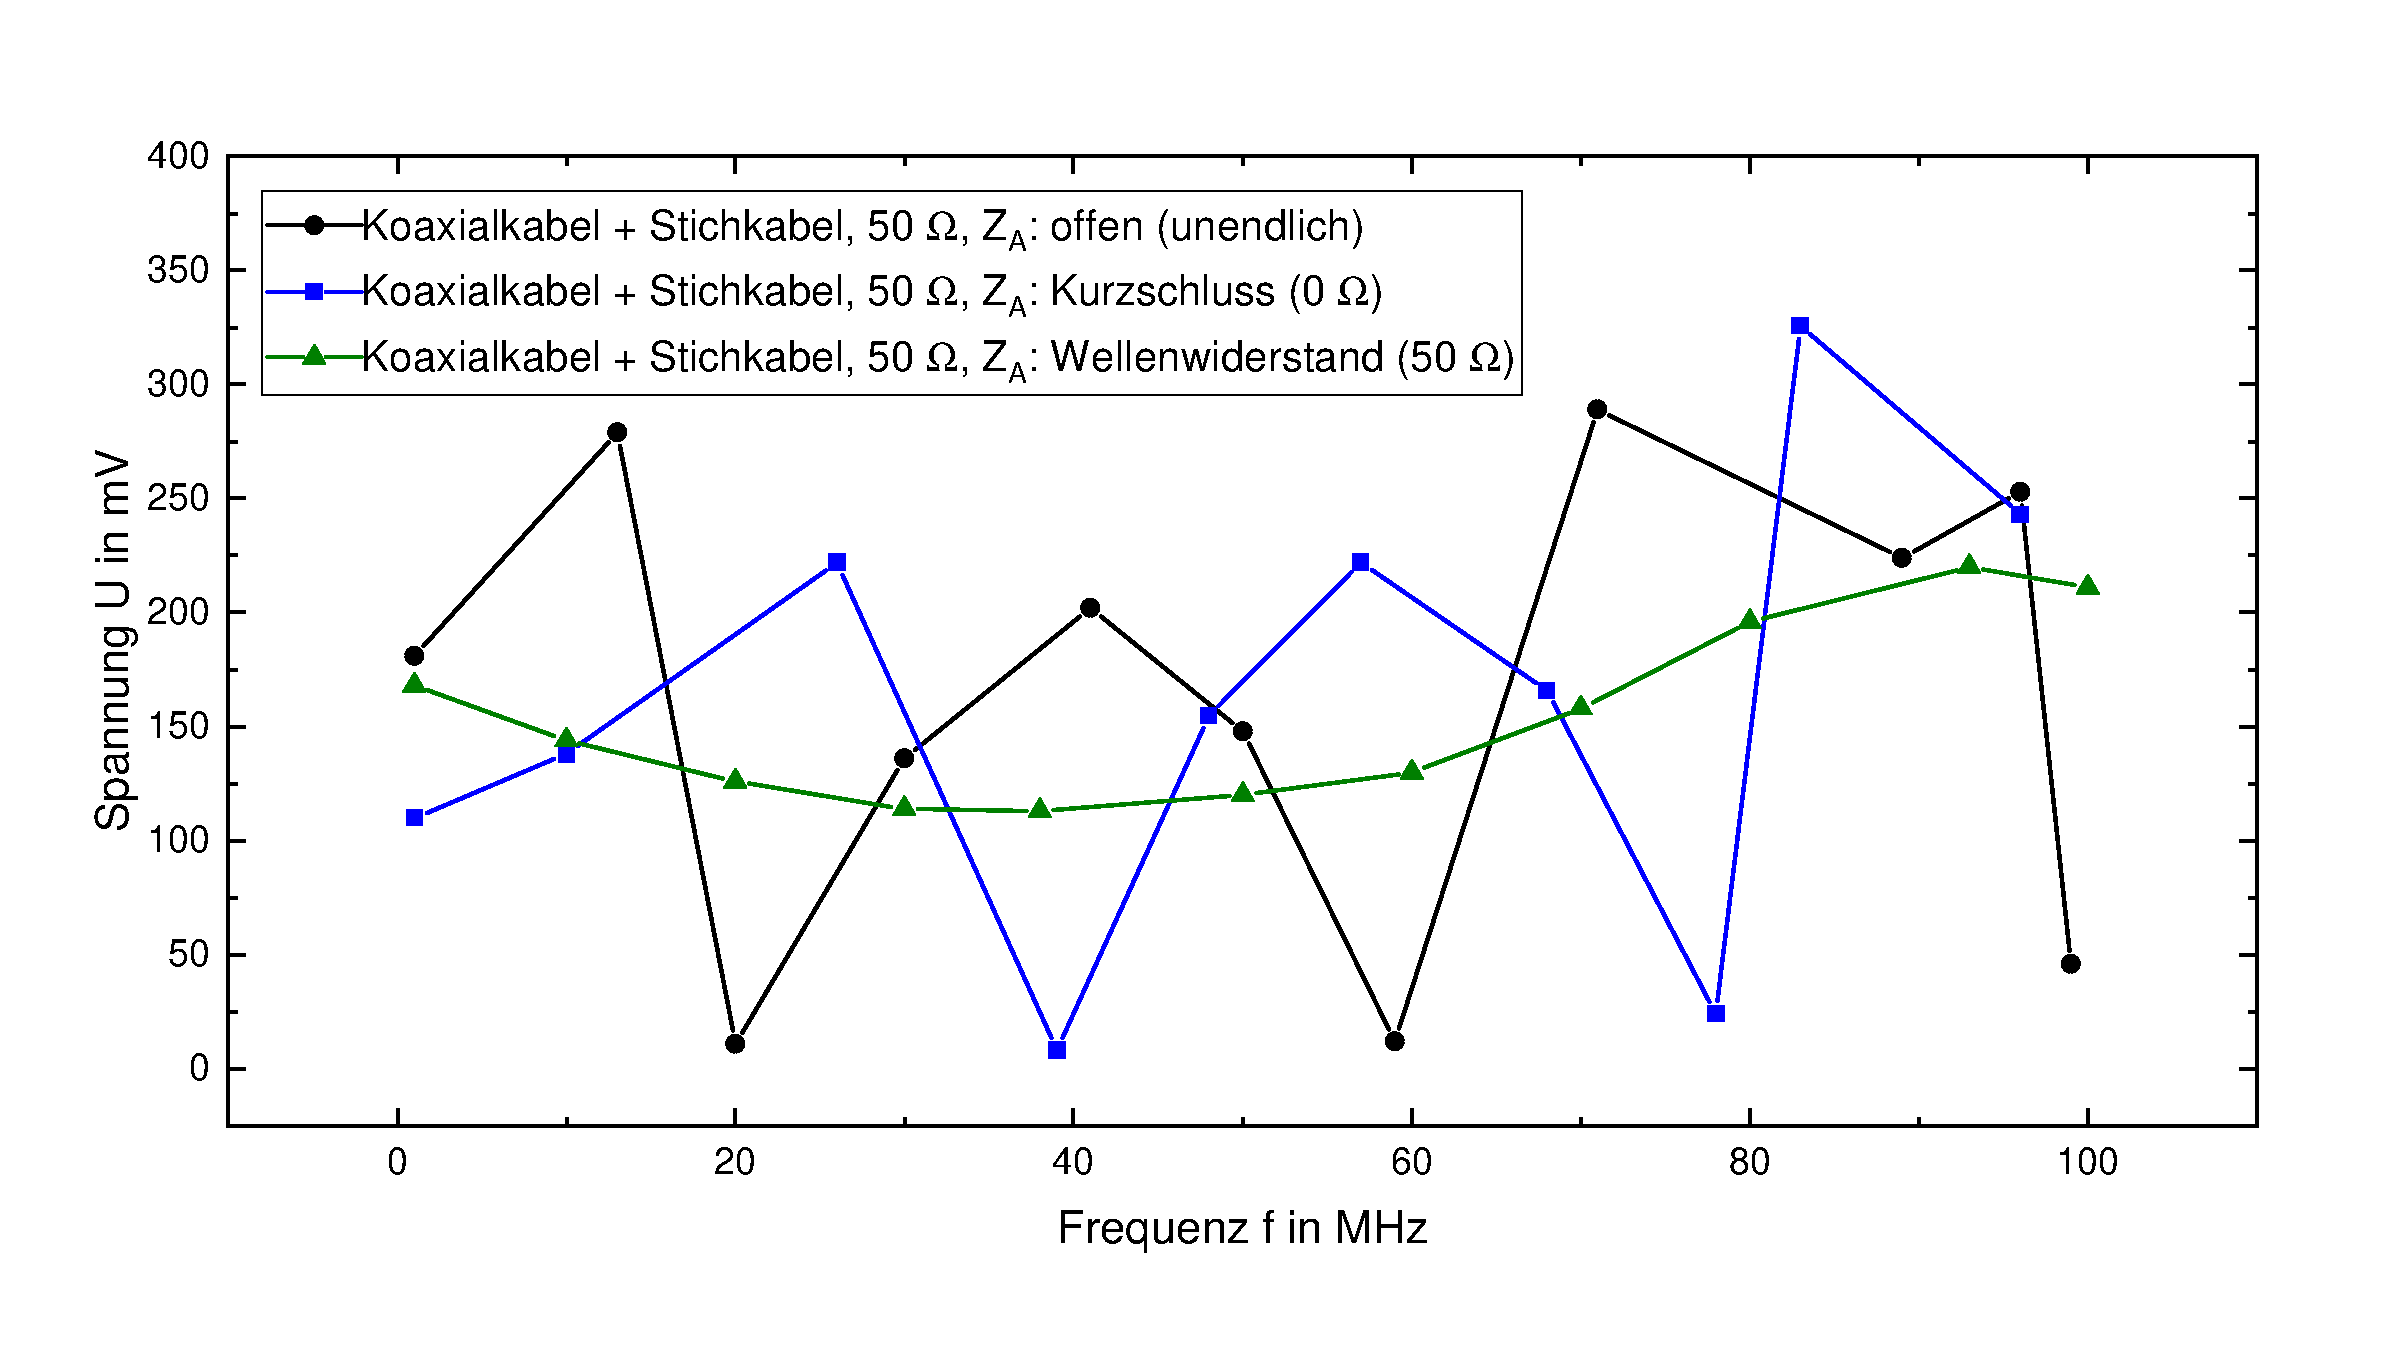
\includegraphics[width=0.9\textwidth]{Bilder/Koaxialkabel_Stichkabel.pdf}
        \vspace{-0.25cm}
    \caption{Frequenzgang von Koxialkabel mit Stichkabel als Verbindung zwischen Generator und Scope (Eingangswiderstand \SI{50}{\ohm} und \SI{1}{\mega\ohm}) }
    \label{fig:Frequenzgang_Koaxialkabel_Stichkabel}
\end{figure}\\
Zunächst wird der Fall des unendlichen Abschlusswiderstands betrachtet. Für diesen Fall muss sich am Ende des Kabels ein Spannungsmaximum befinden. Am Anfang des Kabels ist, als Bedingung für ein Minimum, die Spannung nährungsweise auf \SI{0}{\volt} abgefallen. Da die Spannung sich über die Länge des Kabels sinusförmig verhält, ergibt sich, dass diese Bedingung bei
\begin{align}\label{equ:1/4,3/4}
  L_{\text{Stichk.}} = \frac{\lambda_{L}}{4} \quad \text{und} \quad L_{\text{Stichk.}} = \frac{3\cdot \lambda_{L}}{4}  \quad \Rightarrow \text{allgemein:}\quad L = \frac{(2n+1)\cdot \lambda_{L}}{4}
\end{align}
erfüllt ist, was demnach die Bedingung für ein \textit{Minimum} bei $Z_A = \infty$ darstellt.\\
Soll nun ein Maximum bei $Z_A = \infty$ beschrieben werden, ist folgende Überlegung anzustellen: Auch hier muss wegen $Z_A=\infty$ am Ende des Kabels ein Spannungsmaximum auftreten. Am Anfang des Kabels, als Bedingung für ein Maximum, tritt ebenfalls ein Spannungsmaximum auf. Bei Annahme eines sinusförmigen Verhaltens des Spannungsverlaufs über die Länge des Kabels, ergibt sich, dass diese Bedingung bei
\begin{align}\label{equ:1/2, 1}
L_{\text{Stichk.}} = \frac{\lambda_{L}}{2} \quad \text{und} \quad L_{\text{Stichk.}} = \lambda_{L} \quad \Rightarrow \text{allgemein:}\quad L = \frac{n \cdot \lambda_{L}}{2}
\end{align}
erfüllt ist, was demnach die Bedingung für ein \textit{Maximum}  bei $Z_A = \infty$ darstellt.\\
Bei einem Abschlusswiderstand von $Z_A = \SI{0}{\ohm}$ wird am Ende der Leitung die Spannung nährungsweise auf \SI{0}{\volt} abgefallen sein. Wird hierbei ein Minima gefordert, muss am Anfang des Kabels die Spannung ebenfalls auf \SI{0}{\volt} abgefallen sein. Diese Bedingung ist bei Annahme eines sinusförmigen Verlaufs erfüllt, wenn \eqref{equ:1/2, 1} gilt. Dies entspricht also der Bedingung für ein \textit{Minimum} bei $Z_A = \SI{0}{\ohm}$.\\
Für ein Maximum, wird die Bedingung gestellt, dass die Spannung am Anfang des Kabels ein Maximum erreichen soll. Bei Annahme, dass die Spannung am Ende des Kabels nährungsweise \SI{0}{\volt} ist (da $Z_A = \SI{0}{\ohm}$) und eines sinusförmigen Verlaufs der Spannung entlang des Kabels, finden sich hier die Bedingungen \eqref{equ:1/4,3/4}
Dies entspricht also der Bedingung für ein \textit{Maximum}  bei $Z_A = \SI{0}{\ohm}$.\\
Weiterhin wird anhand der Messdaten festgestellt, dass obwohl mit einem \SI{50}{\ohm}-Stecker am Ende des Stichkabels die Widerstandsanpassung erreicht wird, keine konstante Spannung über alle Frequenzen beobachtet wird. Dies kann an leichten Abweichung des Steckers von \SI{50}{\ohm} und des Kabels von \SI{50}{\ohm} Wellenwiderstand liegen. So treten trotz der scheinbaren Anpassung leichte Reflexionen auf. \\
Es wird festgehalten, dass mit einem Stichkabel nach obigem Prinzip bewusst Frequenzen gefiltert werden können. Für $Z_\text{L, Kabel} = Z_A$ wird der frequenzunabhängigste Frequenzgang erreicht.\\

Zur \textit{Bestimmung des Verkürzungsfaktors} wird das erste Minimum der Spannung bei Verwendung des Stichkabels mit offenem Ende betrachtet. Dieses wird bei \SI{20}{\kilo\hertz} bestimmt. Aufgrund vorheriger Überlegungen entspricht dies genau $\frac{\lambda_{L}}{4}$. Der Verkürzungsfaktor wird bestimmt durch
\begin{align}\label{equ:K}
K = \frac{\lambda_{L}}{\lambda_0} \quad\Rightarrow\quad K = \frac{\frac{\lambda_L}{4}}{\frac{\lambda_0}{4}} = \frac{\SI{2,48}{\metre}}{\frac{c}{4\cdot f}} = \frac{\SI{2,48}{\metre}\cdot 4 \cdot f}{c} = 0,661.
\end{align}
Über die Relation $K = \sqrt{\varepsilon_R}^{-1}$ lässt sich die \textit{Permitivität} auf
\begin{align}
\varepsilon_R = \frac{1}{K^2} = 2,286
\end{align}
bestimmen. Die \textit{Ausbreitungsgeschwindigkeit} ergibt sich durch
\begin{align}
c = \frac{c_0}{\sqrt{\varepsilon_R}} = c_0 \cdot K = \SI{198300000}{\metre\per\second\squared}.
\end{align}
 Mithilfe dieser Werte wird es möglich, eine rechnerische Überprüfung der Bedingung für Minima und Maxima durchzuführen:\\
 Bei näherungsweise unendlichem Abschlusswiderstand ($Z_A = \infty$) können bei
 \SI{20}{\mega\hertz} und \SI{60}{\mega\hertz} Minima beobachtet werden. Diese Beobachtung soll im Folgenden exemplarisch überprüft werden. Es gilt:
 \begin{align}
   \lambda_{L}  = \frac{c_{L}}{f} \quad \text{und} \quad c_{L} = \frac{c_0}{\sqrt{\varepsilon_R}} = c_0 \cdot K
 \end{align}
 Für das Koaxialkabel gilt nach \ref{equ:K} näherungsweise
 \begin{align}
   K = \frac{2}{3}.
 \end{align}
 Damit ergibt sich $\lambda_{L}$ zu
 \begin{align}
 \lambda_{L} = \frac{c_0 \cdot K}{f} = \frac{2 \cdot 10^8}{f}.
 \end{align}
 Bei Betrachtung der $\nu_\text{min}$ wird festgestellt, dass Minima dort auftreten, wo \eqref{equ:1/4,3/4} gilt und Maxima finden sich bei einem Stichkabel mit offenem Ende und Einsetzen der $\nu_\text{max}$ bei \eqref{equ:1/2, 1}.\\
 Allgemein lassen sich folgende \textit{Bedingungen für das Auftreten von Minima und Maxima bei einem Stichkabel der Länge L mit } $Z_A = \infty$ formulieren:
 \begin{align}
 L &= \frac{(2n+1)\cdot \lambda_{L}}{4\cdot f} \; (\text{Minima}) & L &= \frac{n \cdot \lambda_{L}}{2} \; (\text{Maxima}).
 \intertext{Für ein Stichkabel der Länge L mit $Z_A = \SI{0}{\ohm}$ lässt sich entsprechend formulieren:}
 L &= \frac{n \cdot \lambda_{L}}{2} \; (\text{Minima}) & L &= \frac{(2n+1)\cdot \lambda_{L}}{4\cdot f} \; (\text{Maxima}).
 \end{align}

\subsubsection{Verhalten von Rechtecksignalen}
\paragraph{Rechtecksignal über \SI{2}{\metre} langes Koaxialkabel}
Es wurde ein Rechtecksignal an das Scope übertragen bei verschiedenen Eingangswiderständen aufgenommen. Die erhaltenen Darstellungen sind nicht in Abbildung~\ref{fig:Rechtecksignal_Koaxialkabel} im gleichen Maßstab abgebildet.
\begin{figure}[h]
  \centering
  \begin{subfigure}{0.45\textwidth}
    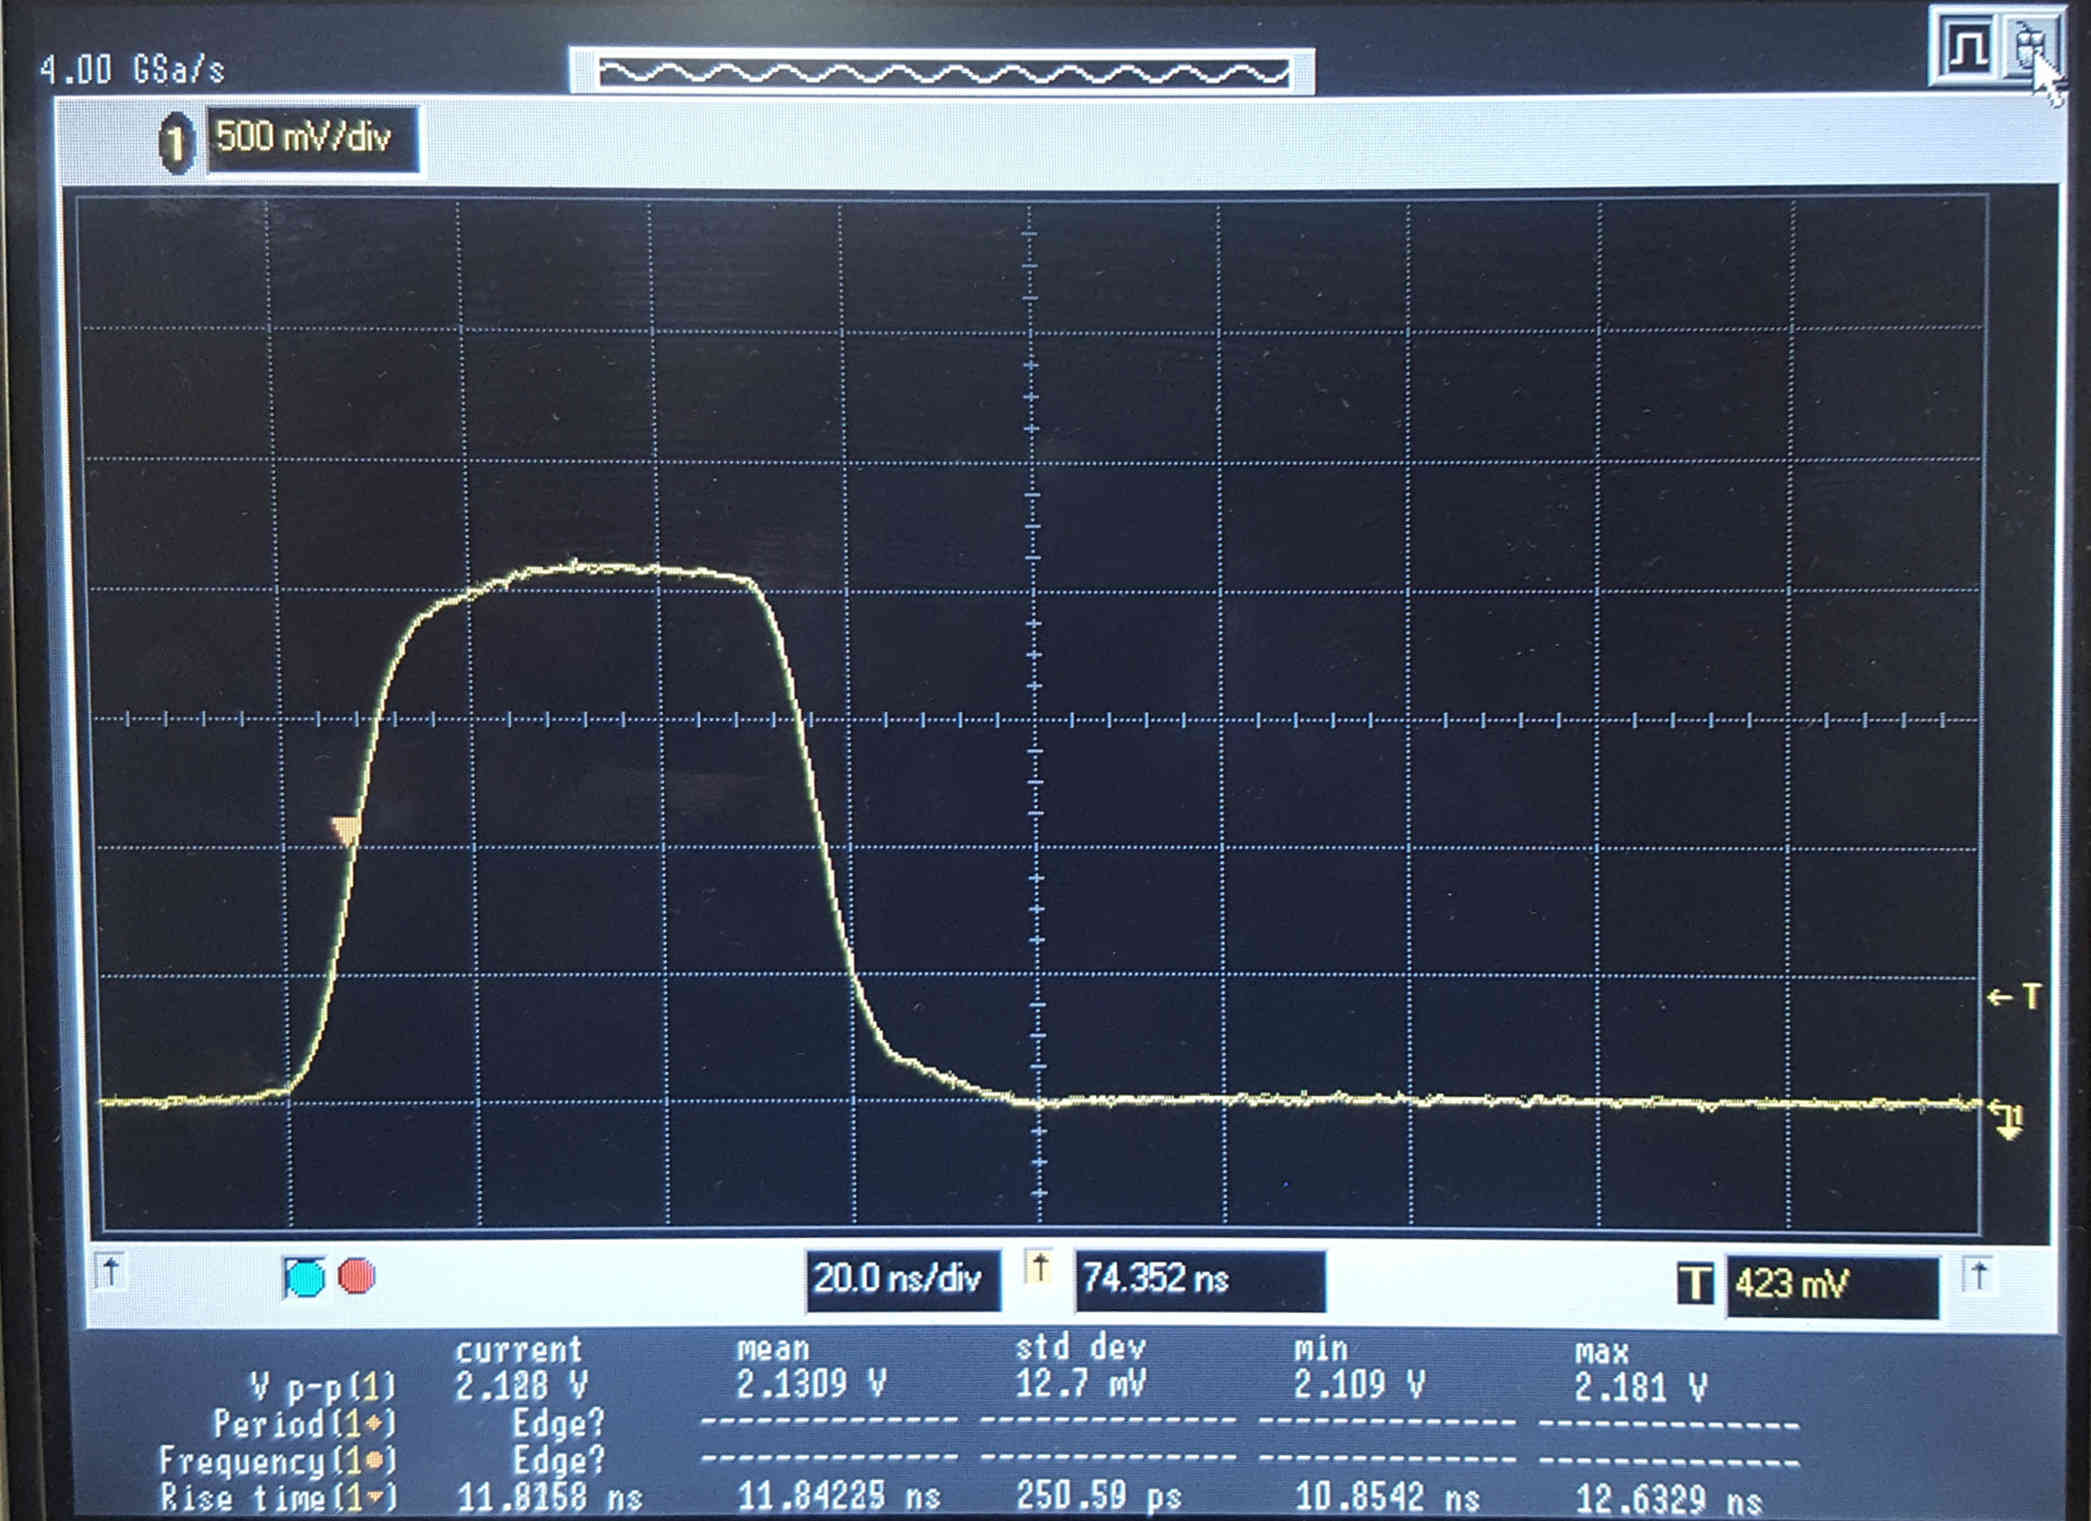
\includegraphics[width=\textwidth]{Bilder/Bild1.jpg}
    \caption{Eingangwiderstand \SI{50}{\ohm}}
  \end{subfigure}\hspace{1cm}
  \begin{subfigure}{0.45\textwidth}
    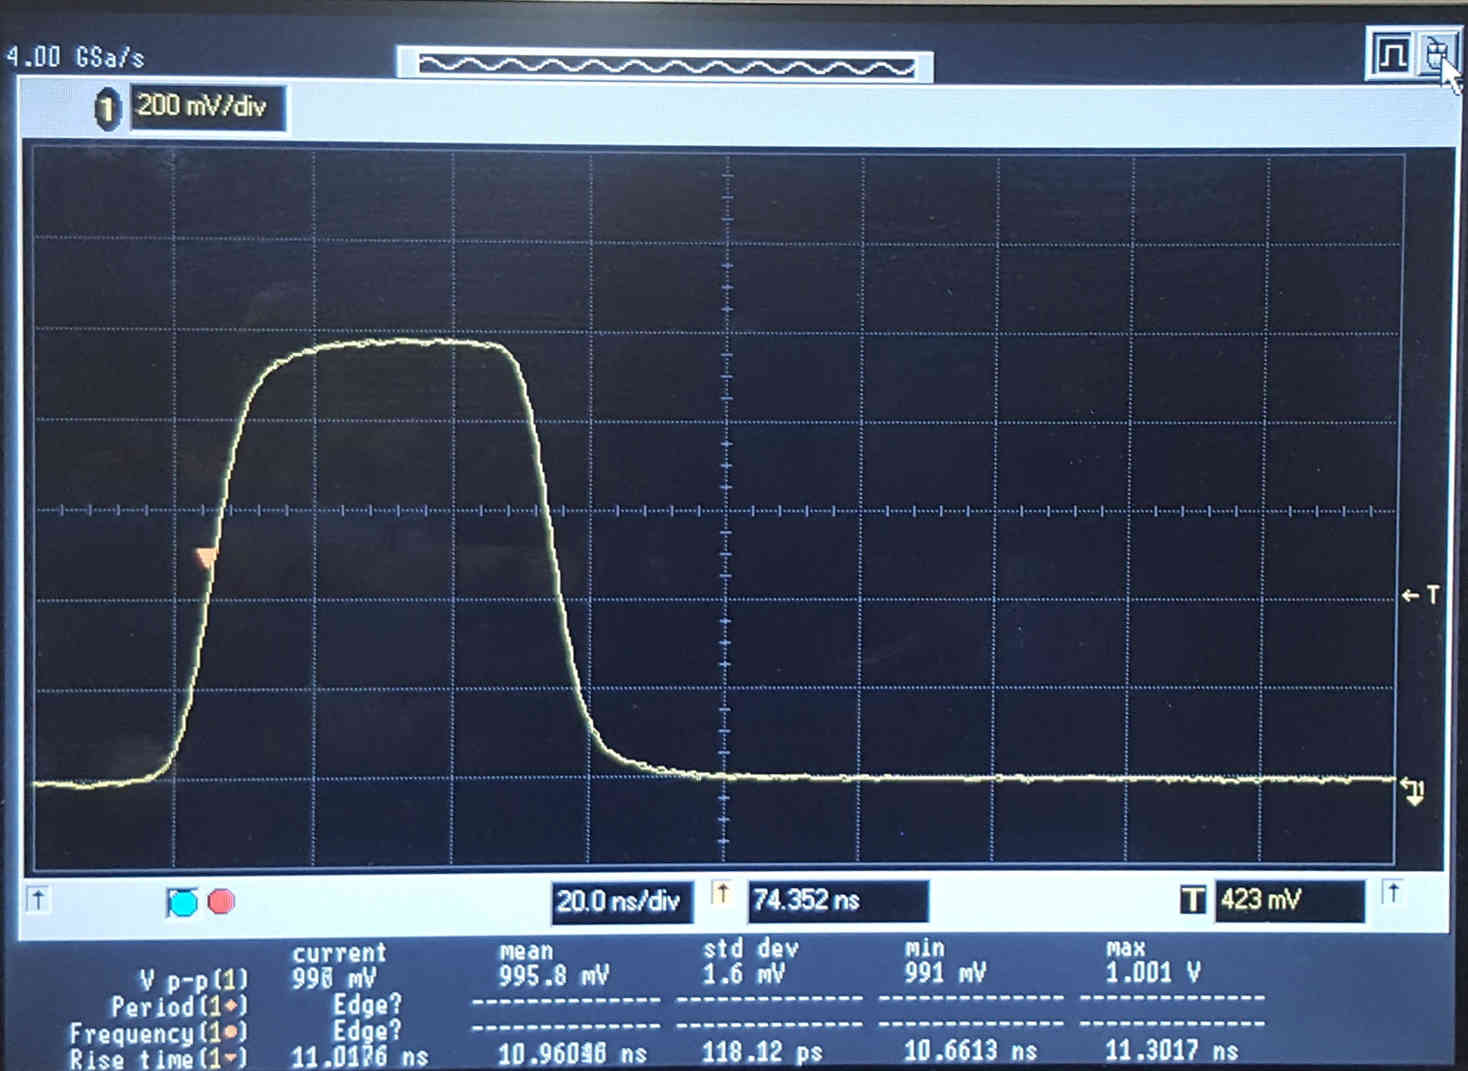
\includegraphics[width=\textwidth]{Bilder/Bild2.jpg}
    \caption{Eingangswiderstand \SI{1}{\mega\ohm}}
  \end{subfigure}
  \caption{Übertragung des Rechtecksignals über \SI{2}{\metre} lange Koaxialkabel bei unterschiedlichen Eingangswiderständen des Scopes}
  \label{fig:Rechtecksignal_Koaxialkabel}
\end{figure}\\
Zum besseren Vergleich wurde die Verstärkung erhöht und der Offset korrigiert um einen qualitativen Vergleich zu ermöglichen. In diesem wird festgestellt, dass bei dem Rechtecksignal, das mit einem, beim Scope eingestellten, Eingangswiderstand von \SI{50}{\ohm} aufgenommen wurde, die Flanken steiler sind, als bei dem Rechteckpuls, das mit dem Scope beim Eingangwiderstand von \SI{1}{\mega\ohm} beobachtet wurde.

\paragraph{Rechtecksignal \SI{25}{\metre} Stichkabel}\label{par:Stichkabel}
Es wurde an das Verbindungskabel ein \SI{25}{\metre} langes Stichkabel mit den Abschlusswiderständen $Z_A = \infty $, $Z_A = \SI{0}{\ohm}$ und $Z_A = Z_L$ angeschlossen und ein Eingangswiderstand von $\SI{50}{\ohm}$ am Scope gewählt. Zum Vergleich wurde für $Z_A = \infty$ auch ein Bild mit Eingangwiderstand des Scopes von $\SI{1}{\mega\ohm}$ aufgenommen. Hierbei kann festgestellt werden, dass der charakteristische Verlauf der gleiche bleibt, jedoch auf den Pulsen Überschwingungen sichtbar werden, die sich aufgrund der aus der Fehlanpassung resultierender Reflexionen ergeben.
\begin{figure}[htp]
    \centering
    \begin{subfigure}{0.45\textwidth}
        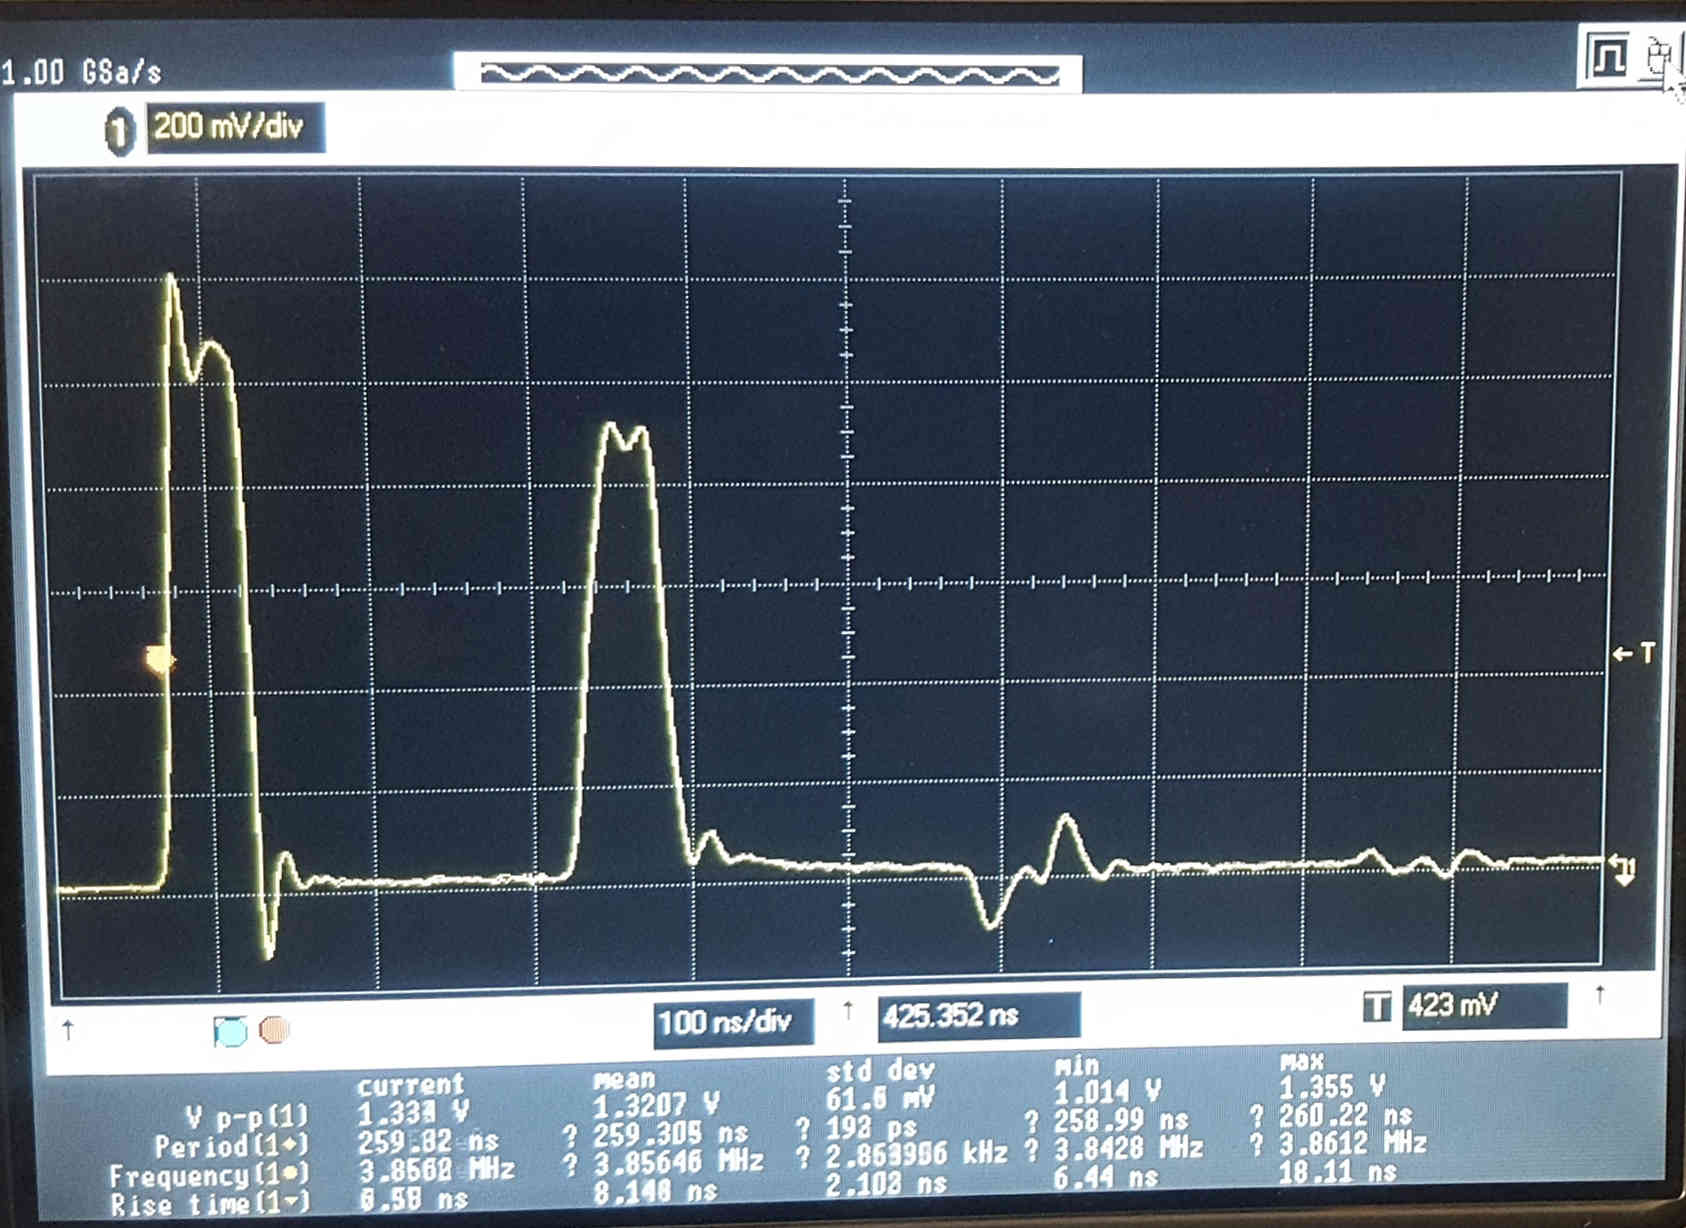
\includegraphics[width=\textwidth]{Bilder/Bild3.jpg}
        \caption{Eingangswiderstand \SI{1}{\mega\ohm}}
    \end{subfigure}\hspace{1cm}
    \begin{subfigure}{0.45\textwidth}
        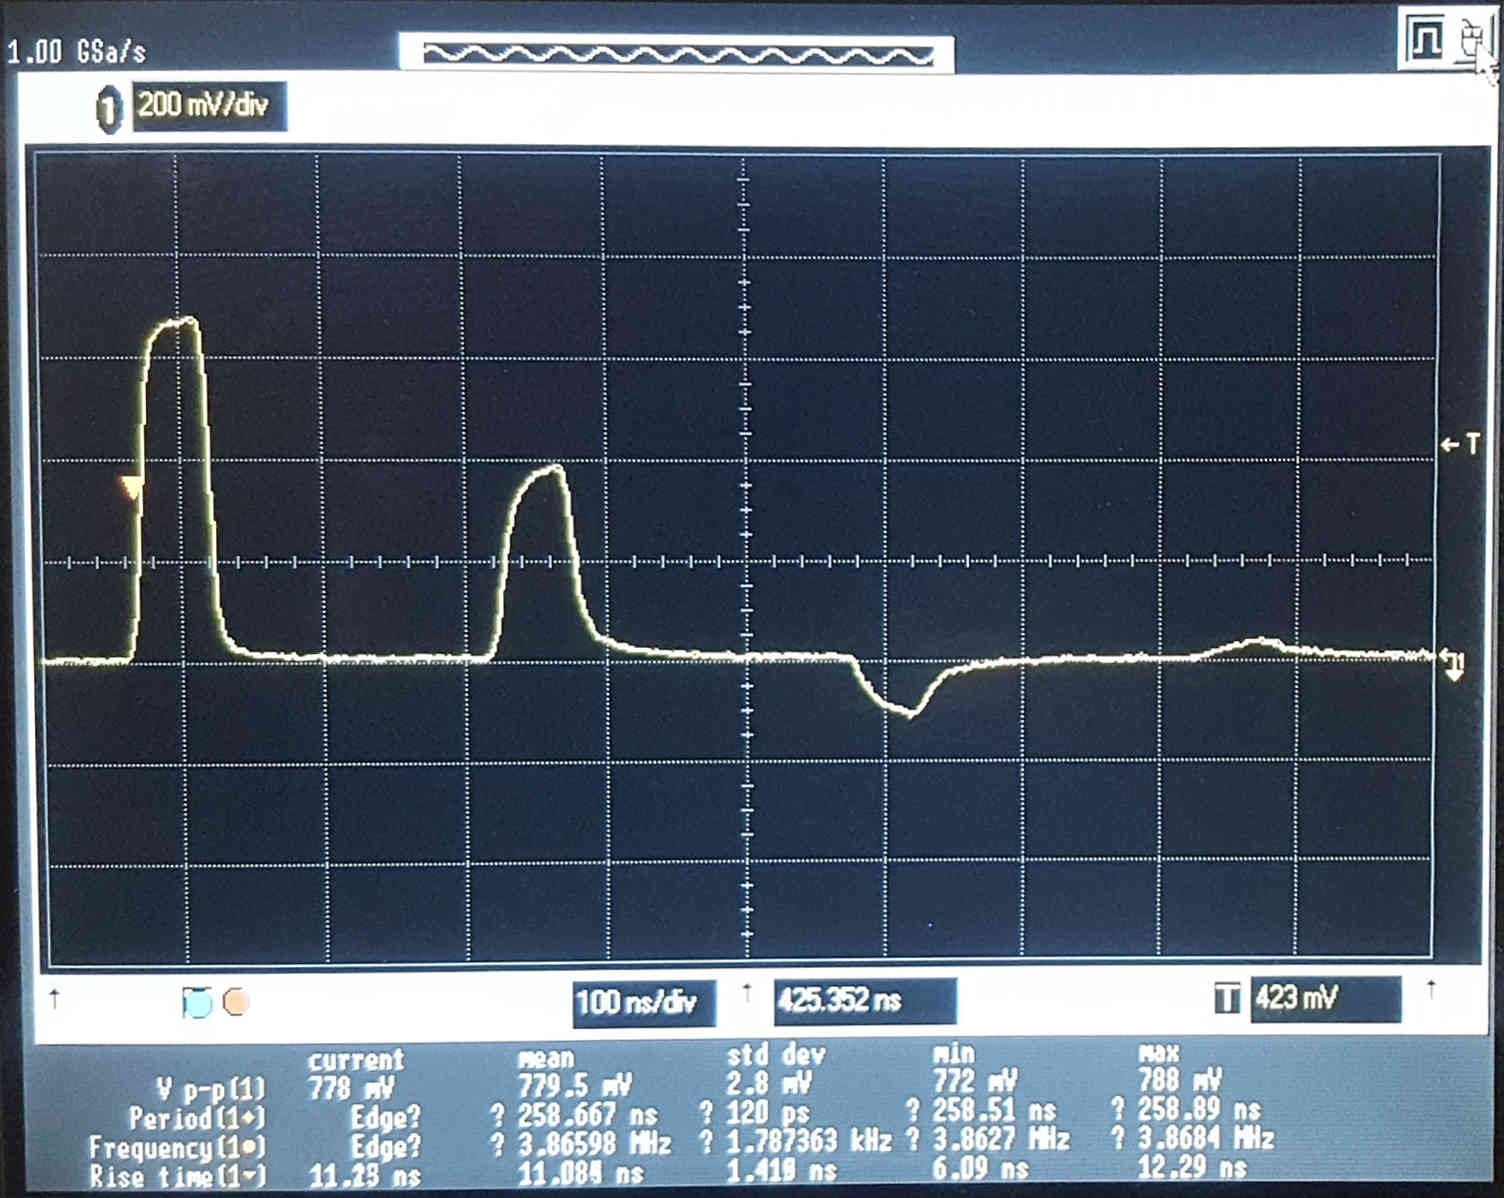
\includegraphics[width=\textwidth]{Bilder/Bild4.jpg}
        \caption{Eingangswiderstand \SI{50}{\ohm}}
    \end{subfigure}
    \caption{Übertragung des Rechtecksignals über \SI{2}{\metre} lange Koaxialkabel mit \SI{25}{\metre} langem Stichkabel mit offenem Ende.}
\end{figure}\\
Für $Z_A = \infty$ (realisiert durch offenes Ende des Stichkabels) können drei Pulse beobachtet werden. Der erste ist der direkt durch das kurze Kabel durchlaufende, unreflektierte Puls. Der zweite Puls stellt den am Ende des Stichkabels reflektierten Puls dar. Dieser ist kleiner und zeigt weniger scharfe Kanten, als der Unreflektierte. Das Aufweichen der scharfen Kanten ergibt sich aus einem Verlust der hohen Frequenzen, welcher aufgrund der längeren Laufzeit dieses Pulses durch das Kabel auftritt. Hierbei erfährt er eine Dämpfung seiner hohen Frequenzen, deren Ursache im frequenzabhängigen Skineffekt liegt. Die Reduktion der Größe lässt sich folgendermaßen erklären: Am Ende des Stichkabels wird der Puls reflektiert und hat zum Zeitpunkt nach der Reflexion noch die fast die gleiche Größe, wie der ursprüngliche Puls. Der Anfang des Stichkabels kann nun auch als Ende eines Kabels aufgefasst werden. Der Abschlusswiderstand hier ergibt sich aus der Parallelschaltung des Widerstand des Scopes und des Frequenzgenerators. Dieser resultierende Widerstand ist kleiner, als der Wellenwiderstand der Leitung, weshalb es zur Invertierung eines Teils des Pules kommt. Hier wird nur ein Teil invertiert, da der Abschlusswiderstand nicht dem Grenzfall $Z_A = \SI{0}{\ohm}$, sondern einem Zwischenzustand $Z_A \leq \infty$ entspricht. Instantan überlagern der vom Ende des Stichkabels reflektierter rücklaufender Puls mit seinem invertierten Teil. Resultierend darauf ergibt sich ein kleinerer Puls, der auf dem Scope zu sehen ist. Der dritte Puls entspricht dem am Anfang des Stichkabels invertierten und nochmals zum Ende des Stichkabels laufenden Teils des Pulses. Dieser wird am Ende wieder refkletiert, am Anfang dann wieder mit seinem invertierten Anteil überlagert usw.
\begin{figure}[htp]
    \centering
    \begin{subfigure}{0.45\textwidth}
        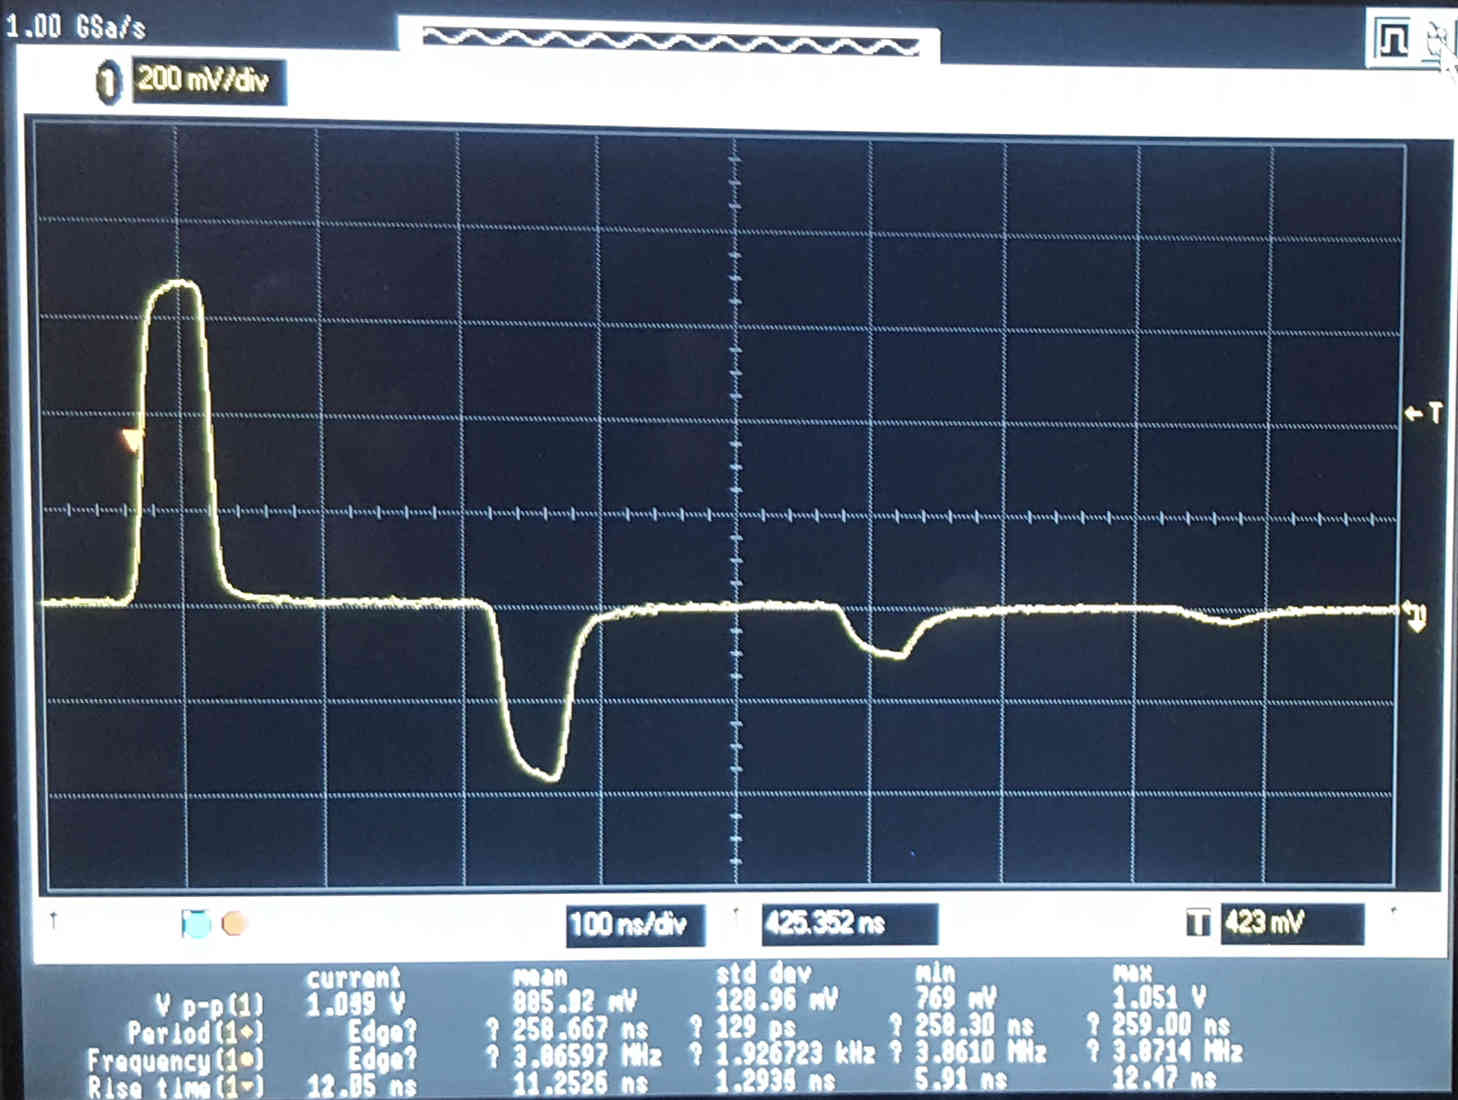
\includegraphics[width=\textwidth]{Bilder/Bild5.jpg}
        \caption{Kurzschlussstecker $Z_A = \SI{0}{\mega\ohm}$}
    \end{subfigure}\hspace{1cm}
    \begin{subfigure}{0.45\textwidth}
        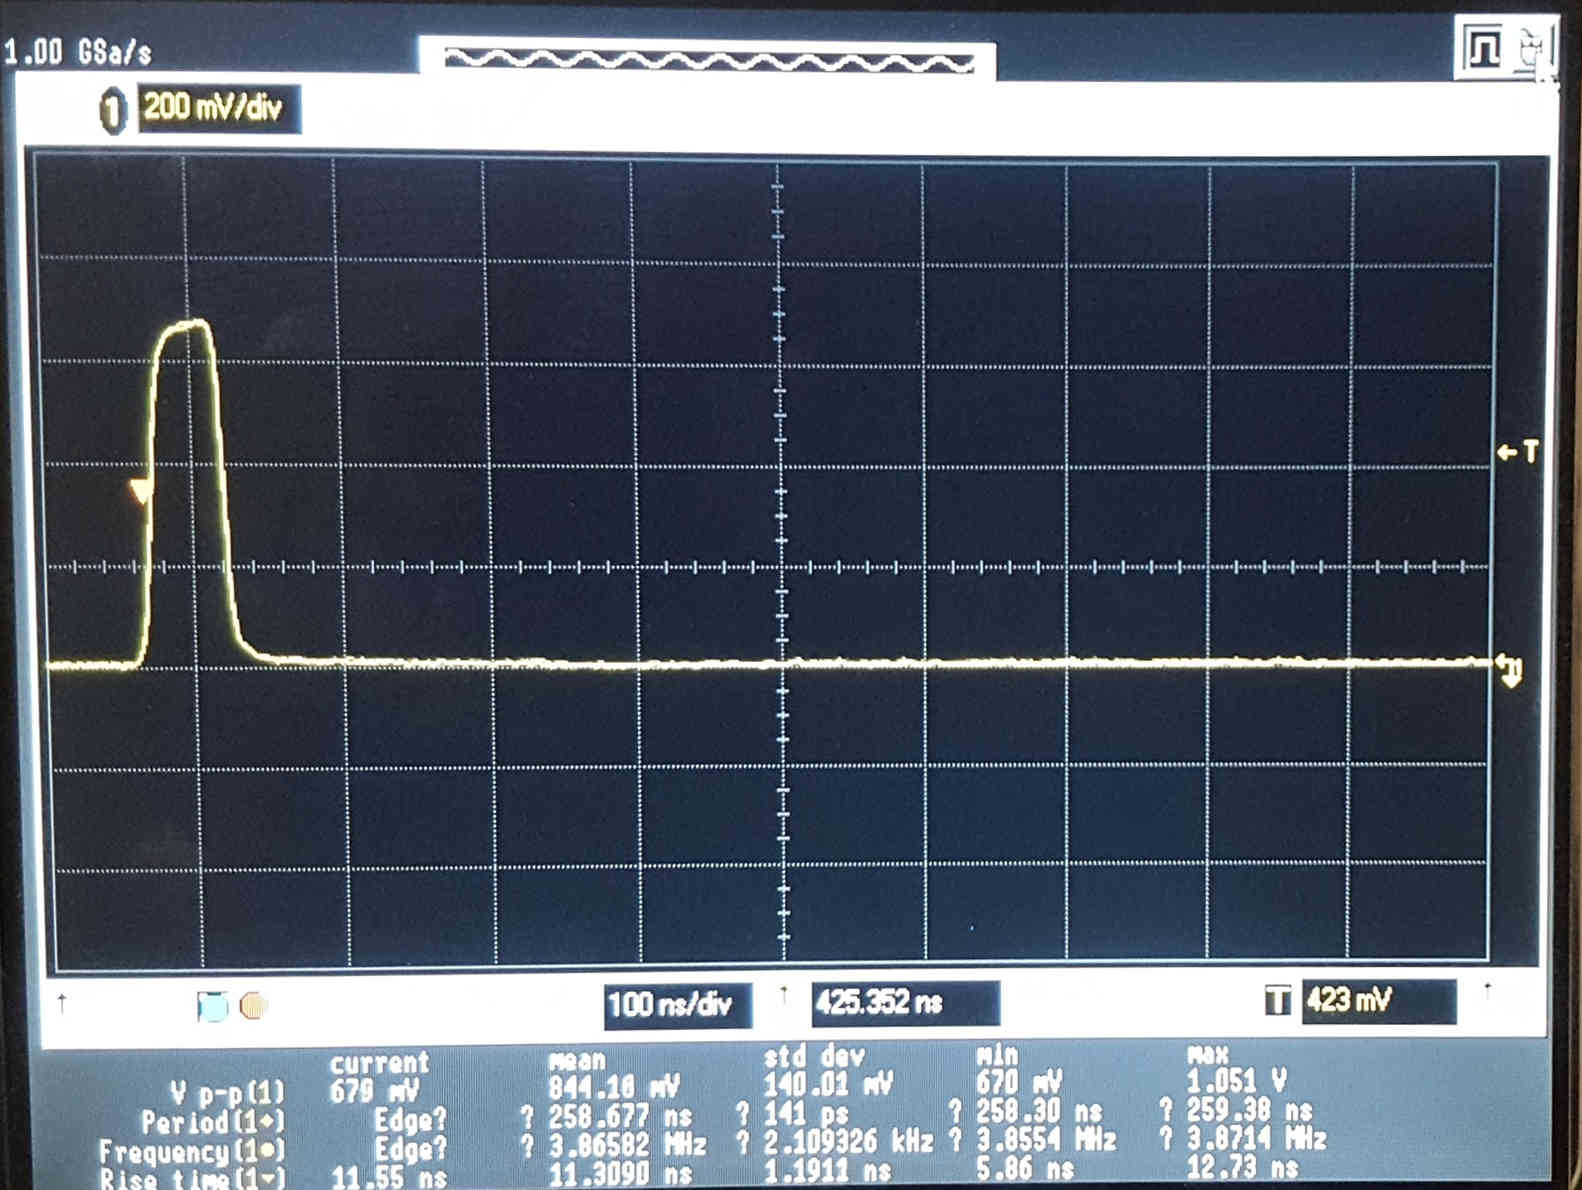
\includegraphics[width=\textwidth]{Bilder/Bild6.jpg}
        \caption{Wellenwiderstandsstecker $Z_A = \SI{50}{\mega\ohm}$}
    \end{subfigure}
    \caption{Übertragung des Rechtecksignals über \SI{2}{\metre} lange Koaxialkabel mit \SI{25}{\metre} langem Stichkabel verschiedener Abshlusswiderstände, Eingangwiderstand Scope: \SI{50}{\ohm}}
    \label{fig:Stichkabel_Kurzschluss_Wellenwiderstand}
\end{figure}\\
Für $Z_A = \SI{0}{\ohm}$, realisiert durch einen Kurzschlussstecker (siehe Abbildung~\ref{fig:Stichkabel_Kurzschluss_Wellenwiderstand} links) können ebensfalls drei Pulse beobachtet werden. Das Prinzip ihrer Entstehung und \glqq Verschmierung\grqq{} ist das gleiche, wie für den ersten diskutierten Fall. Jedoch wird in diesem Fall am Ende des Stichkabels das Signal invertiert, weshalb der zweite Puls negativ ist. \\
Für $Z_A = Z_L$, realisiert durch einen \SI{50}{\ohm}-Stecker, (siehe Abbildung~\ref{fig:Stichkabel_Kurzschluss_Wellenwiderstand} rechts) wird nur der unrefkletierte Puls beobachtet. In diesem Fall wird die Energie des in das Stichkabel laufenden Pulses am Ende des Kabels vom Abschlusswiderstand aufgrund der gewährleiteten Anpassung komplett aufgenommen. Es kommt zu keiner Relfexion, weshalb auch am Scope kein Puls, bis auf den ursprünglichen, zu sehen ist.

\paragraph{Beobachtung des Signals am Ende des Stichkabels }
Beim der Beobachtung des Signals am Ende des Kabels für $Z_A = Z_L$ (realisiert durch Einstellen von \SI{50}{\ohm} für den Eingansgwiderstand) und $Z_A = \infty$ (realisiert durch Einstellen von \SI{1}{\mega\ohm} für den Eingangswiderstand des Scopes)) wird sowohl das Signals am Ende des Kabels (Kanal 1: gelb) als auch das Signal am Ende des Stichkabels (Kanal 2: grün) dargestellt.\\

\begin{figure}[htp]
    \centering
        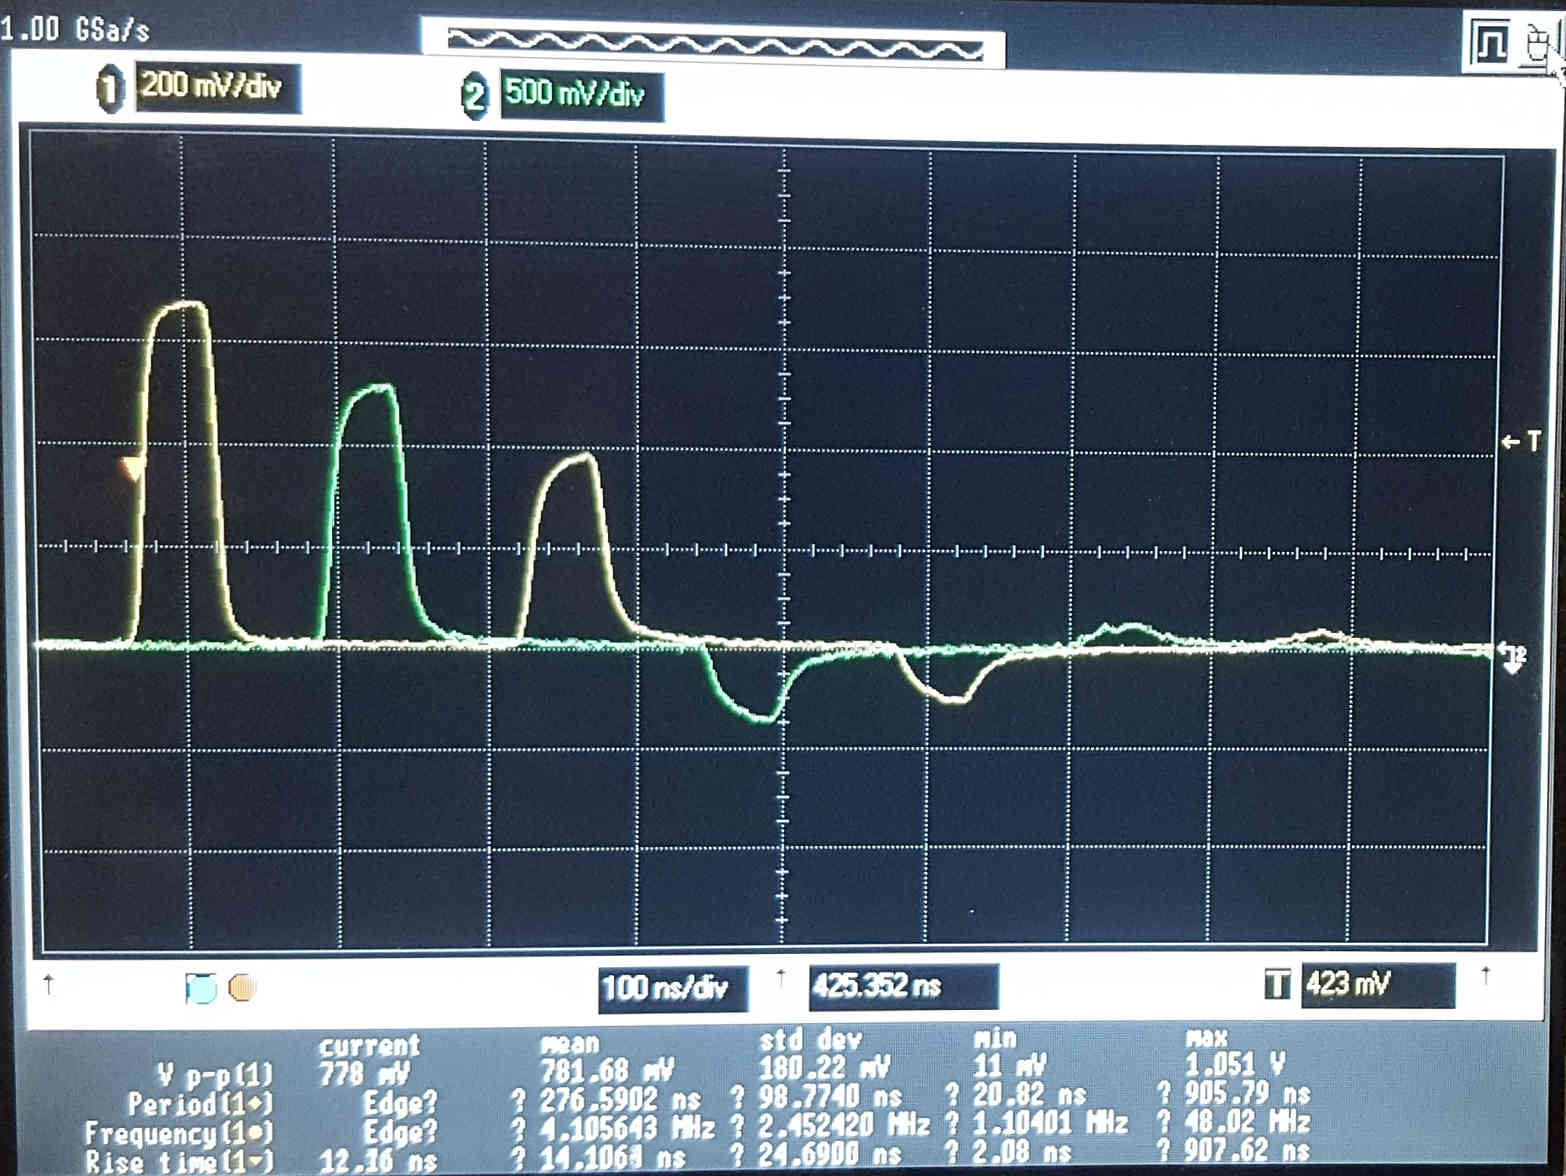
\includegraphics[width=0.45\textwidth]{Bilder/Bild7.jpg}
    \caption{Übertragung des Rechtecksignals über \SI{2}{\metre} lange Koaxialkabel mit \SI{25}{\metre} langem Stichkabel, welches mit dem zweiten Eingang des Scopes verbunden ist (Eingangewiderstand Scope 2. Eingang: \SI{1}{\mega\ohm}), 1. Eingang Scope : \SI{50}{\ohm}}
\end{figure}

Für \textbf{$Z_A = \infty$ am Ende des Stichkabels}(realisiert durch Anschließen des Stichkabels an den zweiten Eingang des Scopes und dortigem Einstellen eines Eingangswiderstandes von \SI{1}{\mega\ohm}) wird deutlich, dass der erste grüne Puls, der am Ende des Stichkabels ankommende, noch größere Puls, ist. Dieser wird dann wie oben beschrieben am Anfang des Stichkabels teiilweise invertiert und überlagert sich direkt mit dem urpsrünglichen rücklaufenden Puls, daraus entsteht dann der zweite gelbe Puls, aber läuft eben auch teilweise invertiert wieder zurück zum Ende des Stichkabels, was dann am zweiten grünen Puls ersichtlich wird. Der dritte gelbe Puls entsteht wie oben beschrieben durch das erneute teilweise Invertieren am Stichkabelanfang und instantanem Überlagern mit den ursprünglich zurücklaufenden Puls. Gleichzeitig wird ein Teil dieses am Stichkabelanfang invertierten Pulses aber auch wieder in das Stichkabel hinein geschickt, woraus sich der dritte grüne Puls ergibt. \\

\begin{figure}[htp]
    \centering
        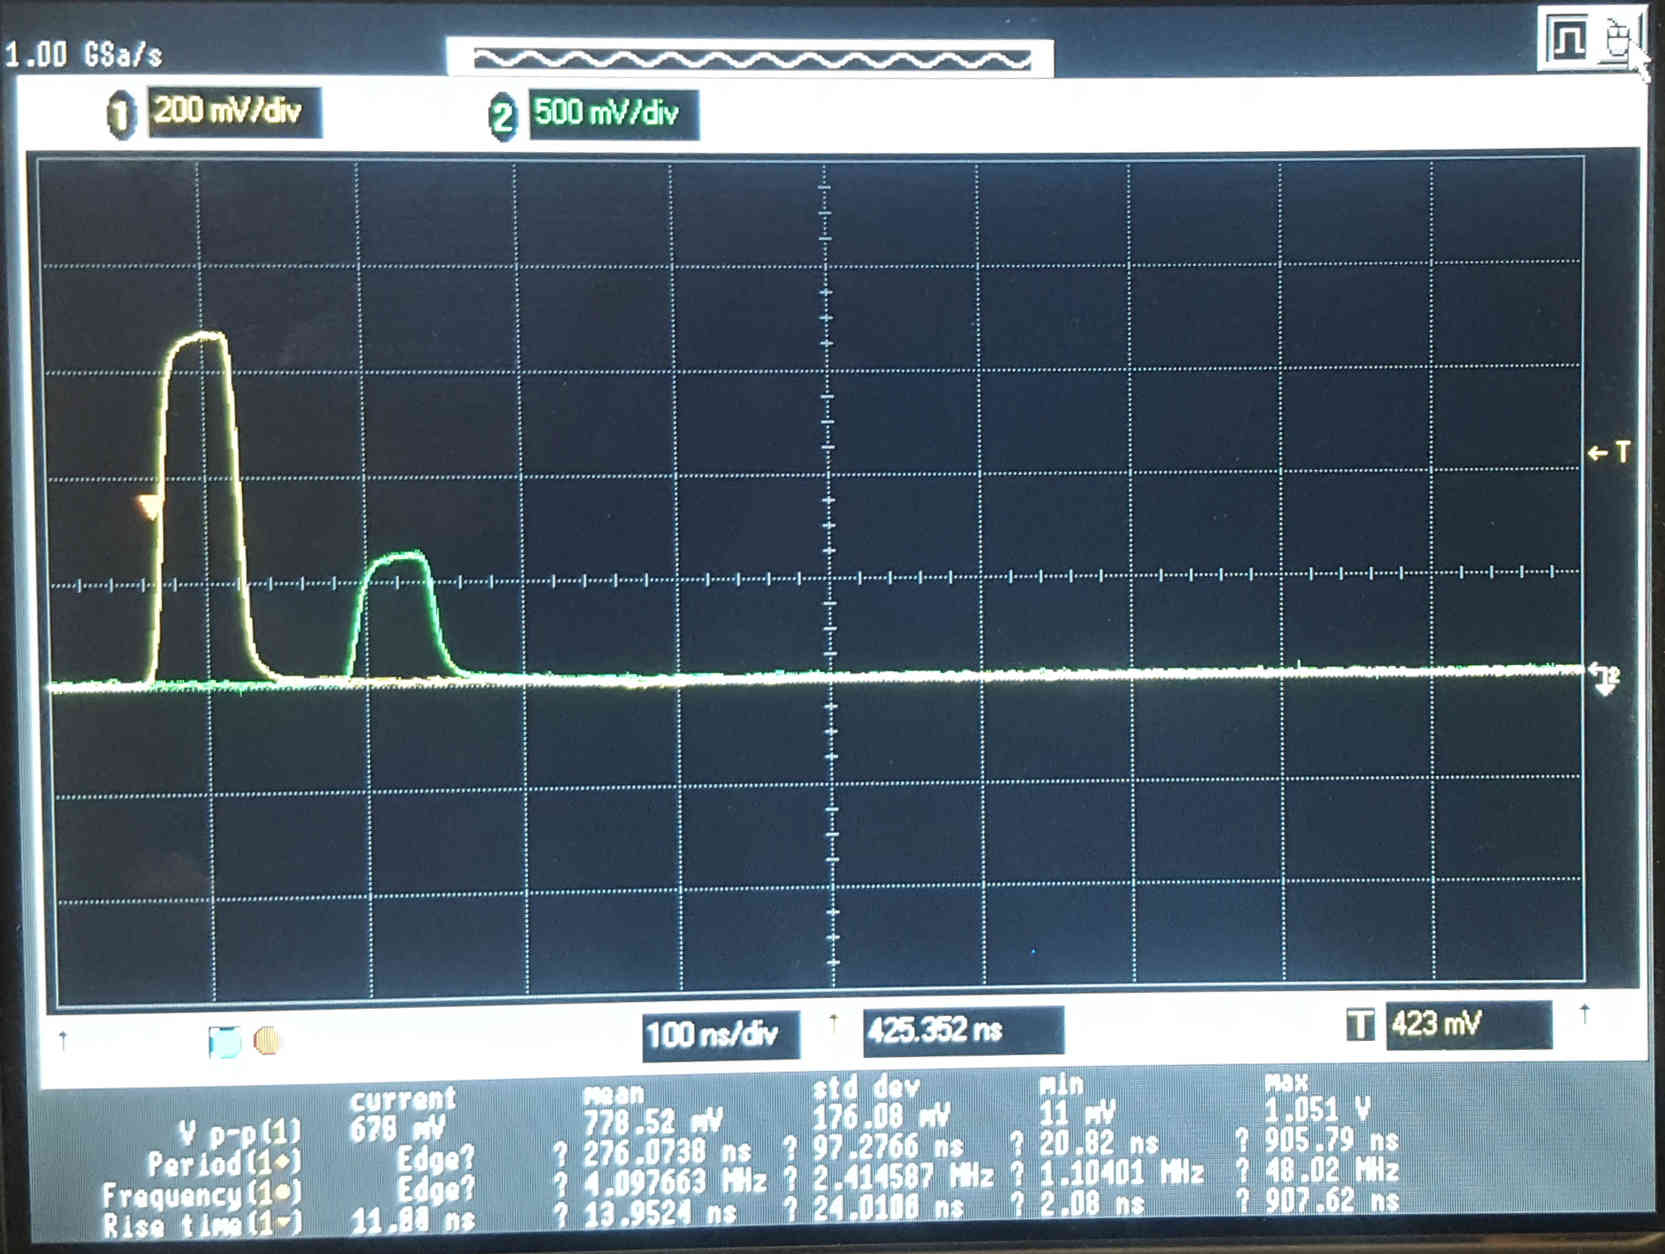
\includegraphics[width=0.45\textwidth]{Bilder/Bild8.jpg}
    \caption{Übertragung des Rechtecksignals über \SI{2}{\metre} lange Koaxialkabel mit \SI{25}{\metre} langem Stichkabel, welches mit dem zweiten Eingang des Scopes verbunden ist (Eingangewiderstand Scope 2. Eingang: \SI{50}{\ohm}), 1. Eingang Scope: \SI{50}{\ohm}}
\end{figure}

Für \textbf{$Z_A = Z_L$ am Ende des Stichkabels}(realisiert durch Anschließen des Stichkabels an den zweiten Eingang des Scopes und dortigem Einstellen eines Eingangswiderstandes von \SI{50}{\ohm}) erschheint am Ende des Stichkabels bereits nur noch ein deutlich kleinerer Puls, der dann von dem Abschlusswiderstand komplett aufgenommen wird.\\

\paragraph{Verwendung einfacher Laborkabel zur Übertragung des Rechteckpulses}

\begin{figure}[htp]
    \centering
    \begin{subfigure}{0.45\textwidth}
        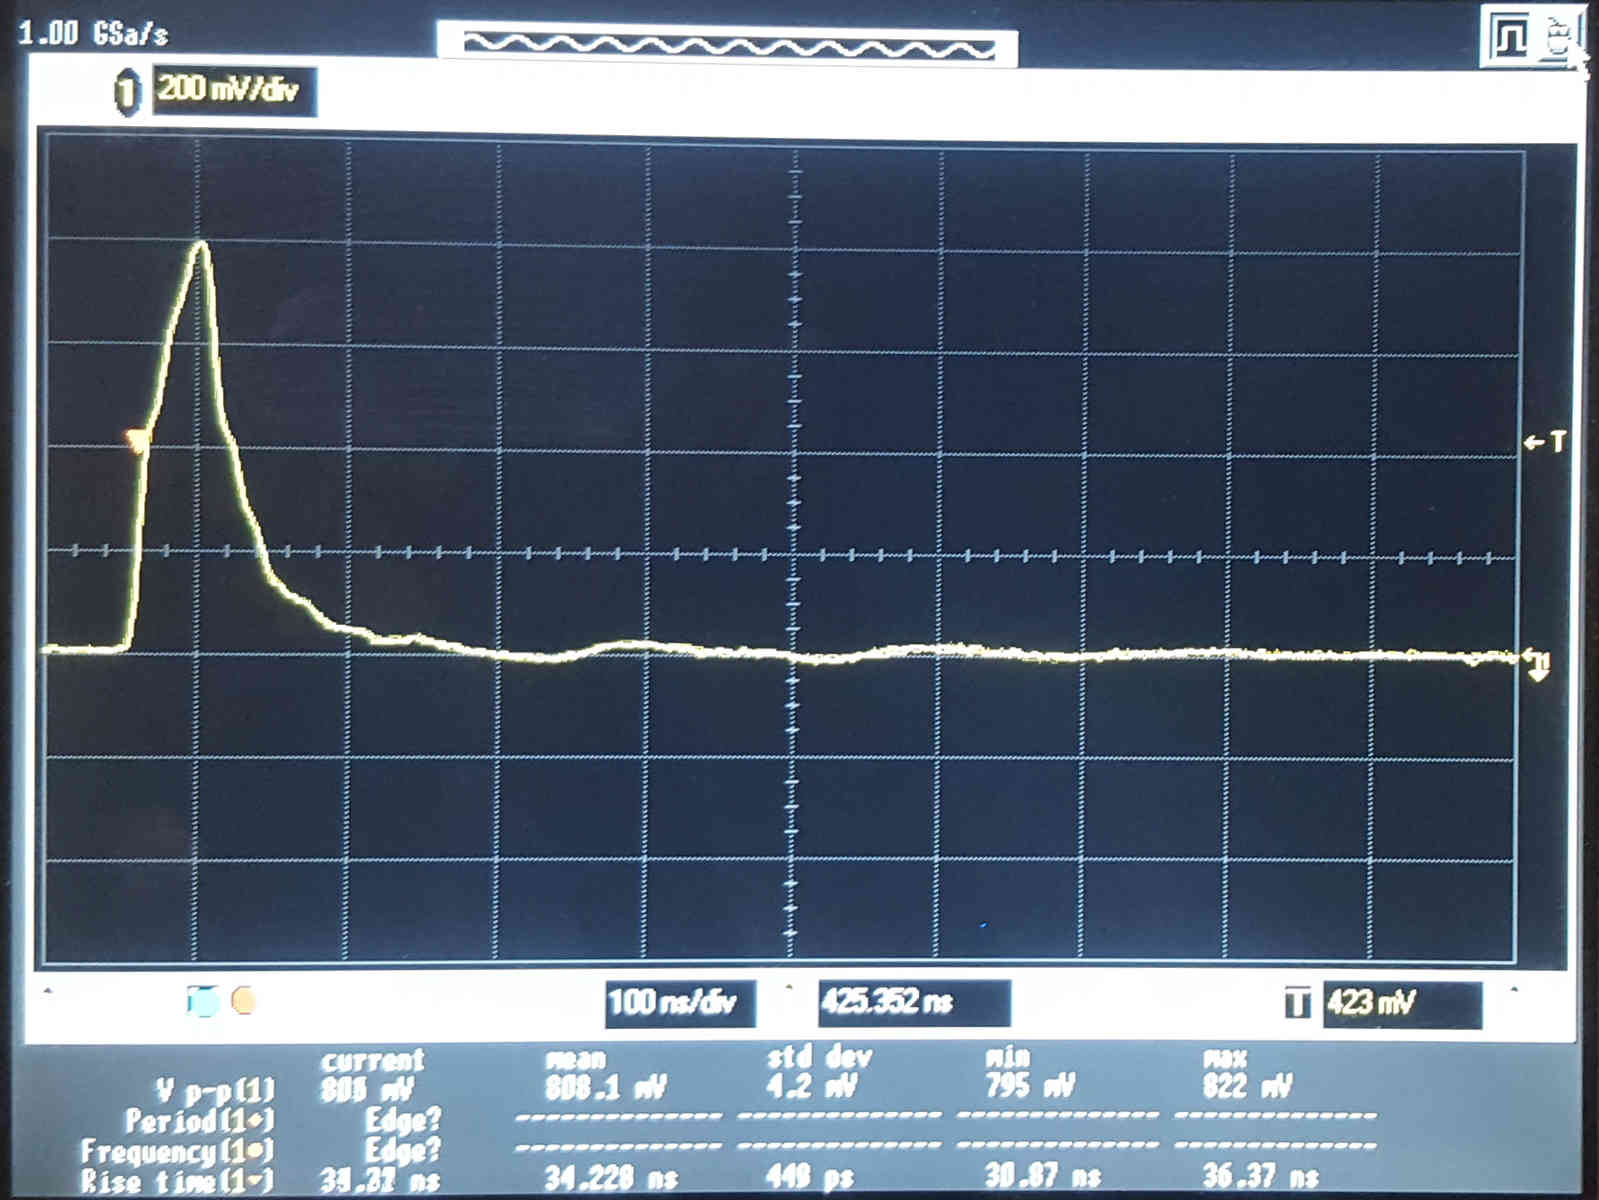
\includegraphics[width=\textwidth]{Bilder/Bild9.jpg}
        \caption{Eingangwiderstand \SI{50}{\ohm}}
    \end{subfigure}\hspace{1cm}
    \begin{subfigure}{0.45\textwidth}
        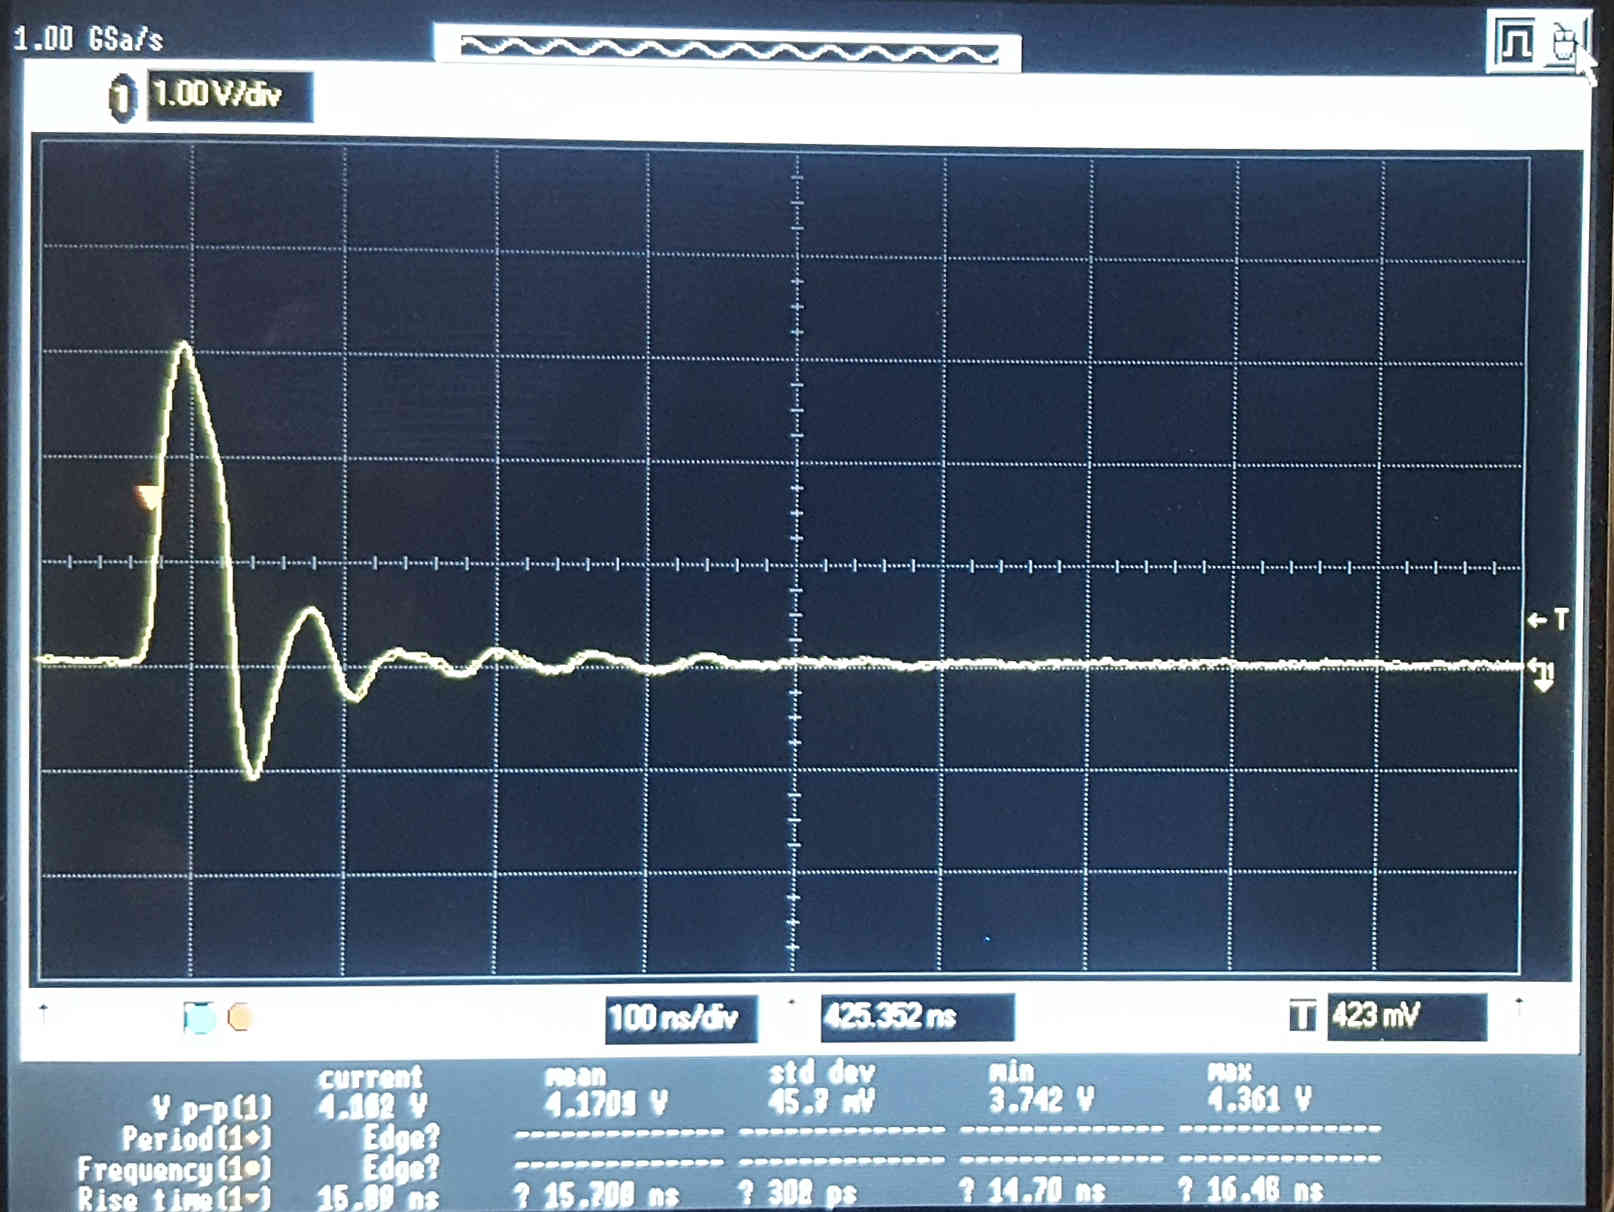
\includegraphics[width=\textwidth]{Bilder/Bild10.jpg}
        \caption{Eingangswiderstan \SI{1}{\mega\ohm}}
    \end{subfigure}
    \caption{Übertragung des Rechtecksignals über \SI{2}{\metre} lange Laborkabel bei unterschiedlichen Eingangswiderständen des Scopes}
\end{figure}

Wird der Rechteckpuls mit einfachen Laborkabeln übertragen, wird auch bei optimaler Einstellung von einem Eingangswiderstand des Scopes von \SI{50}{\ohm} Abschlusswiderstand kein scharfer Rechteckpuls übertragen. Anstattdessen wird auf dem Scope ein Peak erkannt. Die bereits am Anfang des Versuchs aufgenommene chaotische Frequenzabhängigkeit der Spannung kommt hier zum Tragen und macht die Übertragung eines Rechteckpulses, womit die Übertragung vieler Frequenzen verbunden ist, unmöglich. \\
Bei \SI{1}{\mega\ohm} Eingangswiderstand kommen zusätzlich noch die Relektionen dazu. Ein chaotisches Bild zeigt sich, dass für den ungeübten Beobachter den Anschein einer Schwingung macht.
\newpage
\paragraph{Bestimmung der Ausbreitungsgeschwindigkeit, Verkürzungfaktor und Permitivität}
Die Bestimmung erfolgte auf zwei verschiedene Weisen. \\
Zunächst wird der Aufbau genutzt, bei dem ein Stichkabel (Länge: \SI{25}{\metre} mithilfe eines T-Stücks auf das, den Scope mit dem Frequenzgenerator verbindende, Kabel angebracht wird. Dabei werden Messwerte bei offenem Ende des Stichkabels bei \SI{50}{\ohm} sowie \SI{1}{\mega\ohm} und bei Kurzschlusstecker am Ende des Stichkabels bei \SI{50}{\ohm} sowie \SI{1}{\mega\ohm} aufgenommen. Jeweils gemessen wird der Abstand der ersten Flanke des ersten Pulses zur gleichen Flanke des gleichen Pulses. Bei allen Messungen belief sich diese Verschiebung auf:
\begin{align}
\Delta_1 = \SI{255}{\nano\second}
\end{align}

Wird berücksichtigt, dass die Strecke vom T-Stück zum Scope im Vergleich zur Länge des Stichkabels vernachlässigbar klein ist und für die Rechnung nur die doppelte Länge des Stichkabels berücksichtigt werden muss, ergibt sich c zu
\begin{align}
c = \frac{\SI{50}{\metre}}{\SI{255,35}{\nano\second}} = \SI{196e6}{\metre\per\second}
\end{align}

Somit folgt für K
\begin{align}
K = \frac{c}{c_0} = 0,654
\end{align}

und damit für $\varepsilon_R$
\begin{align}
\frac{1}{\sqrt{\varepsilon_R}} = 0,654 \Rightarrow \varepsilon_R = 2,34
\end{align}

Eine andere Möglichkeit besteht darin, die drei Größen über den zuletzt verwendeten Aufbau zu erhalten. Ist das Ende des Stichkabels mit dem Scope (Eingangswiderstand \SI{50}{\ohm}) verbunden und werden erste Flanke des Pulses, der unreflektiert durch geht, mit der ersten Flanke des am Ende des Stichkabels beobachteten Pulses verglichen, ergibt sich deren Verschiebung zu:
\begin{align}
\Delta_2  = \SI{123,68}{\nano\second}
\end{align}

Hierbei ergibt sich c zu
\begin{align}
c = \frac{\SI{24}{\metre}}{\SI{123,68}{\nano\second}}= \SI{194e6}{\metre\per\second}
\end{align}

Für $\varepsilon_R$ und K folgt
\begin{align}
K = 0,647 \qquad \varepsilon_R = 2,39
\end{align}

\paragraph{Wellenwiderstandsbestimmung mit Rechteckimpulsen}
Es wird ein RG58 Koaxialkabels wie in \ref{subsec:BestimmungZL} beschrieben vermessen. So kann der Widerstand auf
\begin{align}
Z_L = \SI{51,6 \pm 0,1}{\ohm}
\end{align}
bestimmt werden.

\paragraph{Wellenwiderstandsbestimmung durch L und C Messung}
Für die Messung mit Kurzschlussstecker am RG58 Koaxialkabels wird ein Wert von
\begin{align}
L = \SI{0,12}{\micro\henry}
\end{align}
für die Induktivität aufgenommen. Für die Messung bei offenem Ende wird ein Wert für die Kapazität von
\begin{align}
C = \SI{35,6}{\pico\farad}.
\end{align}
Damit ergibt sich R zu
\begin{align}
R = \sqrt{\frac{L}{C}} =  \SI{58,0}{\ohm}.
\end{align}
Die Abweichung zum idealen Wellenwiderstand ergibt sich daraus, dass bei der Verwendung des Kurzschlusssteckers nicht exakt $Z_A = \SI{0}{\ohm}$ und bei Offen-Lassen nicht exakt $Z_A = \infty$ erreicht wird.
\subsection{Modulation}
\subsubsection{Simulation mit LabView}
Zuerst wurde mithilfe eines LabView Programms eine Simulation von additiver und multiplikativer Amplitudenmodulation durchgeführt. Dabei wurde eine Nutzfrequenz $\nu_\text{N} = \SI{5}{\kilo\hertz}$ und eine Trägerfrequenz $\nu_\text{T} = \SI{100}{\kilo\hertz}$ zur Simulation des modulierten Signals benutzt.\\
Zunächst wurden die beiden Signale nur addiert, wodurch noch keine Modulation entsteht. Die Verläufe im Zeit- und Frequenzbereich sind in Abbildung~\ref{fig:Addition} dargestellt.
\begin{figure}[htp]
    \centering
    \begin{subfigure}{0.45\textwidth}
        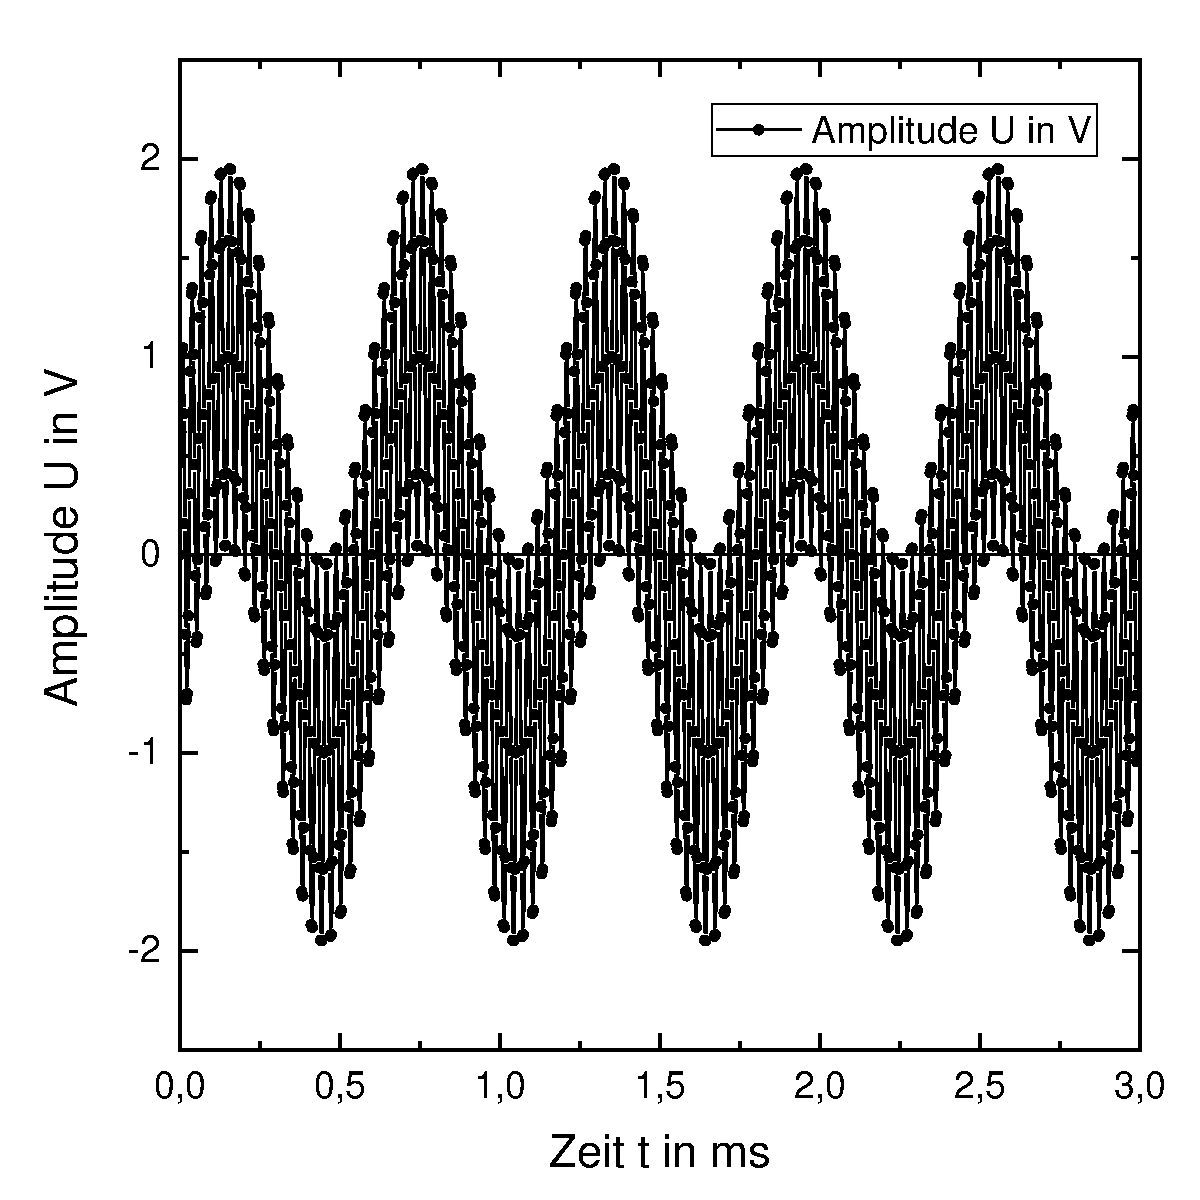
\includegraphics[width=\textwidth]{Bilder/Addition_Zeitverlauf.pdf}
    \end{subfigure}
    \begin{subfigure}{0.45\textwidth}
        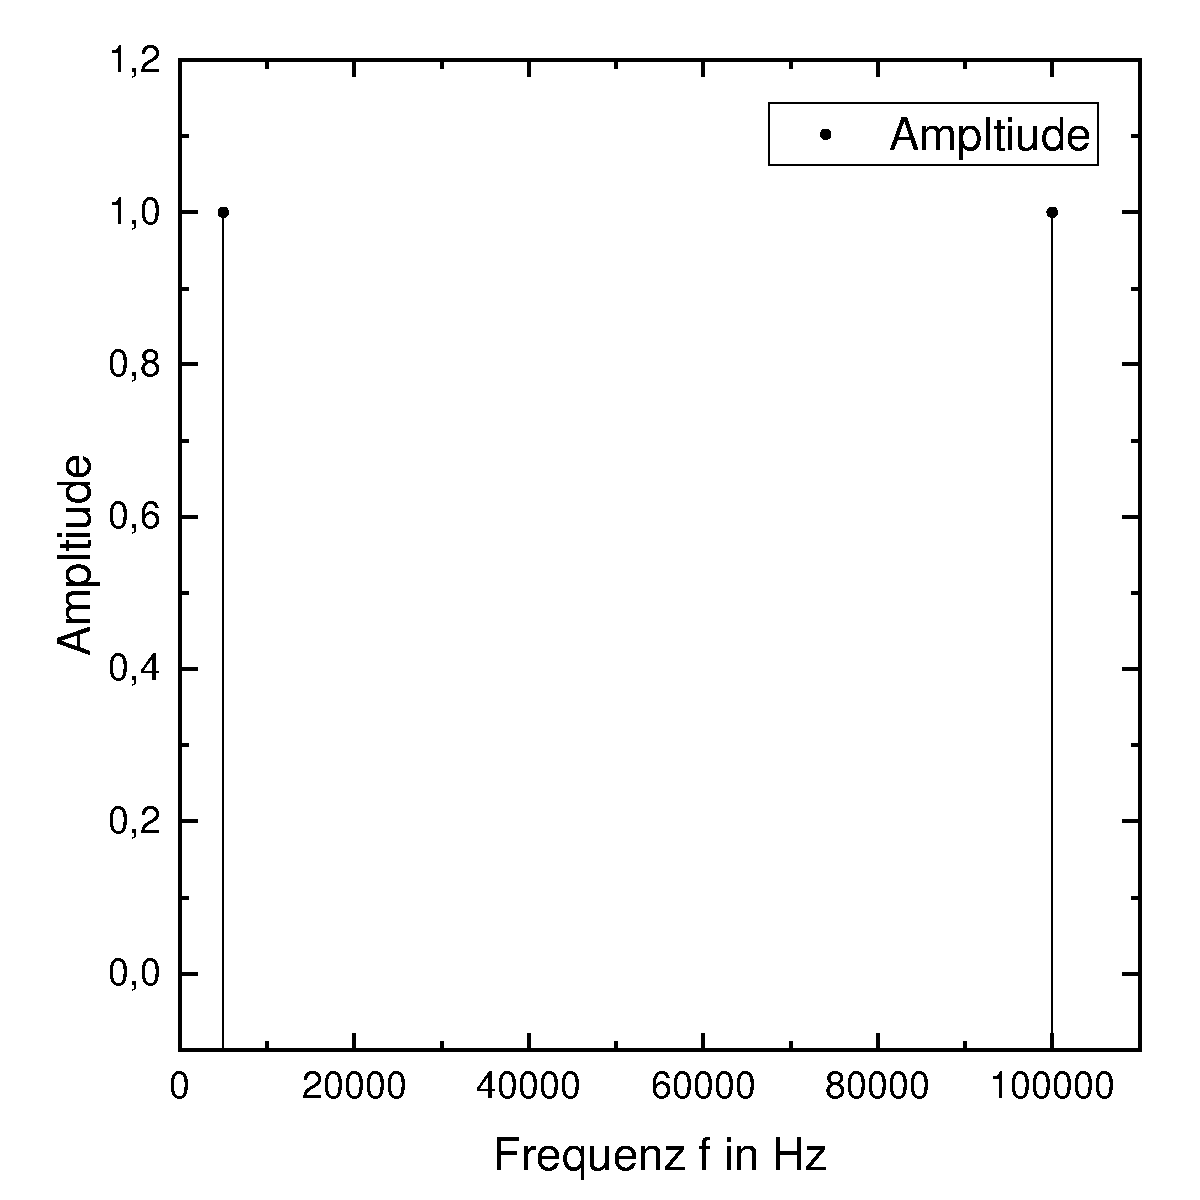
\includegraphics[width=\textwidth]{Bilder/Addition_Frequenzverlauf.pdf}
    \end{subfigure}
    \label{fig:Addition}
    \caption{Zeitverlauf und Frequenzspektrum der addierten Signale nach der Formel $U(t) = \sin(\omega_\text{N}) + a\cdot \sin(\omega_\text{T})$ mit Amplitude $a = \SI{1}{\volt}$.}
\end{figure}\\
Es zeigt sich, dass beide Frequenz wieder im Frequenzbereich auffindbar sind, was verdeutlicht, dass hierbei keine Modulation stattgefunden hat.
\begin{figure}[htp]
    \centering
    \begin{subfigure}{0.45\textwidth}
        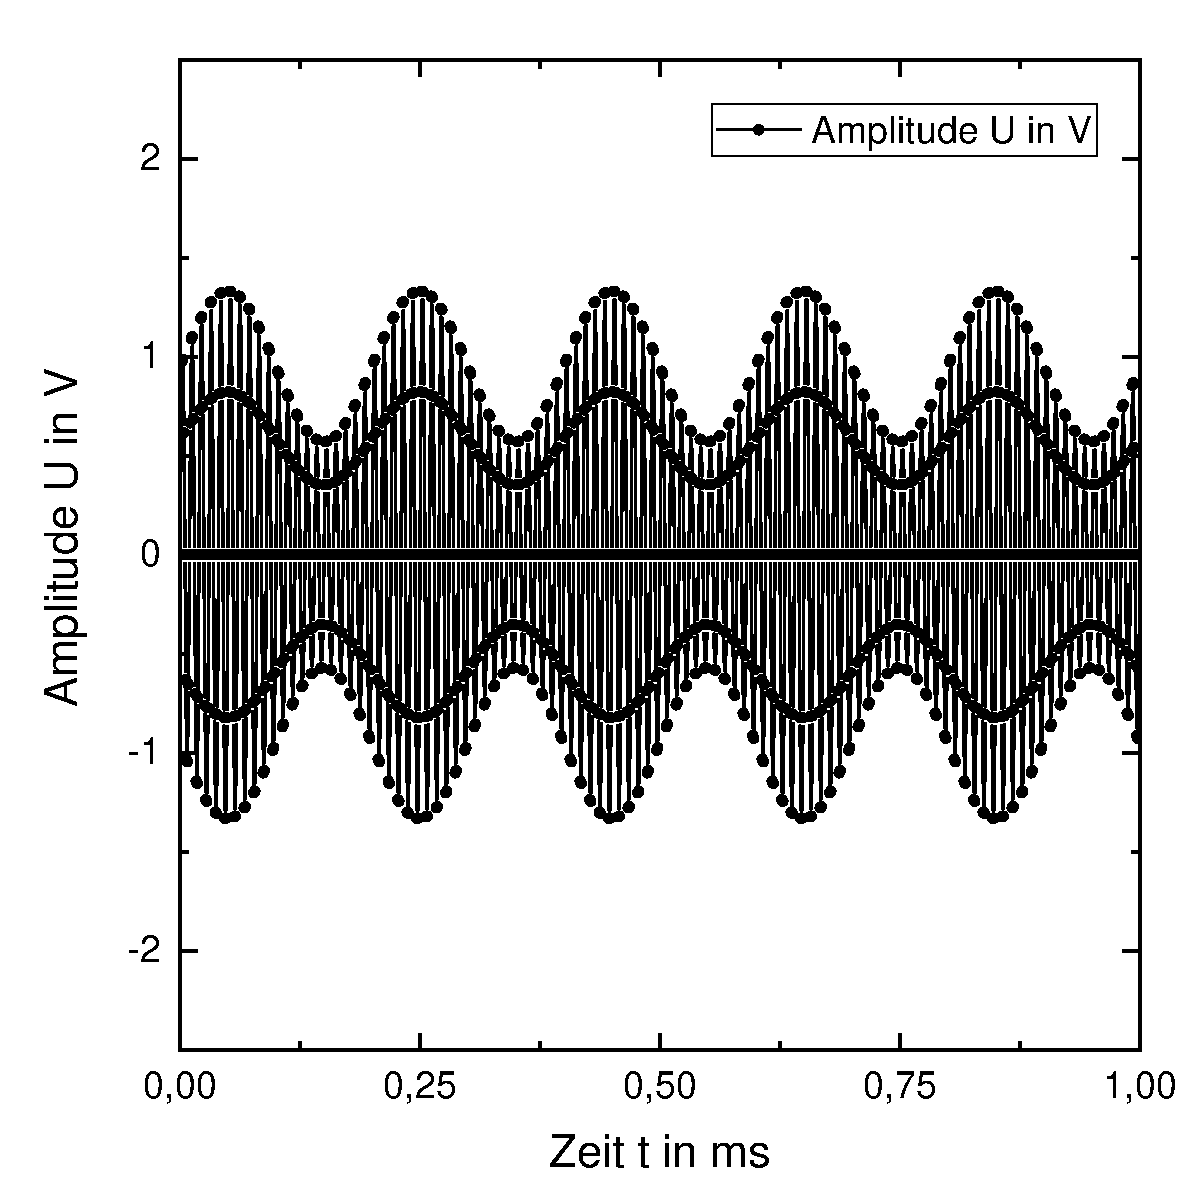
\includegraphics[width=\textwidth]{Bilder/AM1_additiv_Zeit.pdf}
    \end{subfigure}
    \begin{subfigure}{0.45\textwidth}
        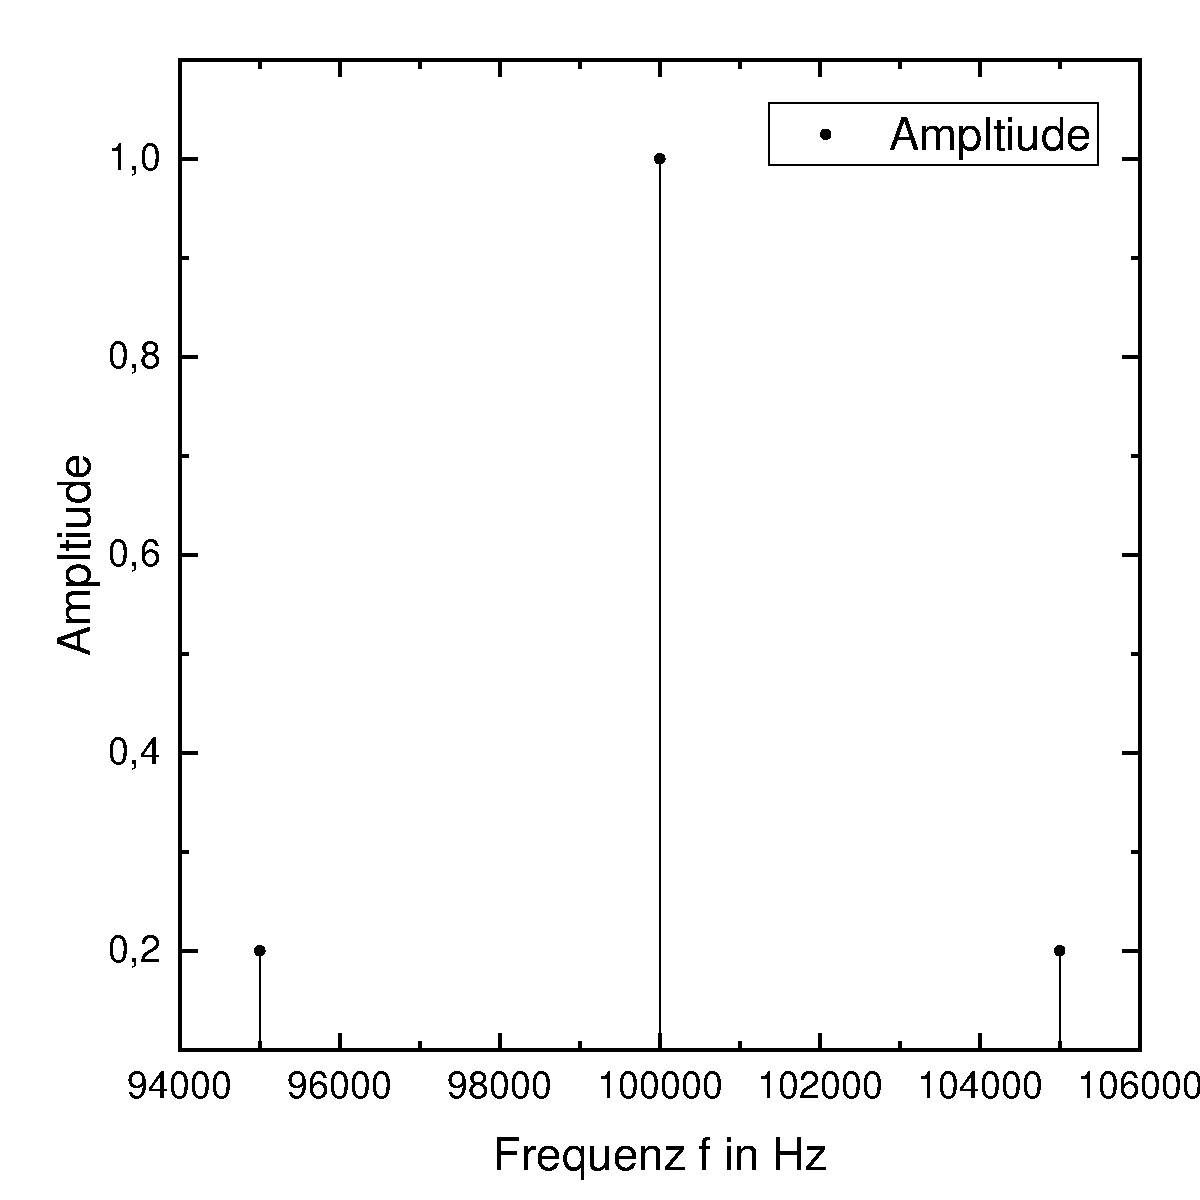
\includegraphics[width=\textwidth]{Bilder/AM1_additiv_Frequenz.pdf}
    \end{subfigure}
    \caption{Zeitverlauf und Frequenzspektrum der additiv amplitudenmodulierten Signale nach Formel \eqref{eqn:AM_additiv} mit Modulationsgrad $M = 0,4$.}
    \label{fig:AM1_additiv}
\end{figure}\\
Weiterhin wurde eine additive Amplitudenmodulation mit verschiedenen Modulationsgraden durchgeführt. Wie zuvor wurden als Nutzfrequenz $\nu_\text{N} = \SI{5}{\kilo\hertz}$ und Trägerfrequenz $\nu_\text{T} = \SI{100}{\kilo\hertz}$ verwendet. Die Amplitude des Nutzsignals wird mit $U_\text{T} = \SI{1}{\volt}$ wird festgehalten. Als Amplitude $U_\text{N}$ des Signals wurden $\SI{400}{\milli\volt}$ gewählt. Damit ergibt sich nach Gleichung~\eqref{eqn:Modulationsgrad} ein Modulationsgrad von $M = 0,4$. Die Ergebnisse der Simulation zeigt Abbildung~\ref{fig:AM1_additiv}.\\
Bei der Betrachtung des Frequenzspektrums erscheint wieder die Trägerfrequenz mit einer hohen Amplitude und symmetrisch im Abstand von $\SI{5}{\kilo\hertz}$ die beiden Seitenbänder $\nu_\text{T}\pm \nu_\text{N}$.\\
Es lässt sich erkennen, dass die Hüllkurve der Modulationsschwingung kein Minimum aufweist. Wird nun wie in Abbildung~\ref{fig:AM2_additiv} (links) ein Modulationsgrad von $M = 1$ gewählt, indem die Amplitude $U_\text{N} = \SI{1}{\volt}$ gesetzt wird, dann sinkt die Amplitude eine einhüllenden Kurve auf $\SI{0}{\volt}$ ab.
\begin{figure}[htp]
    \centering
    \begin{subfigure}{0.45\textwidth}
        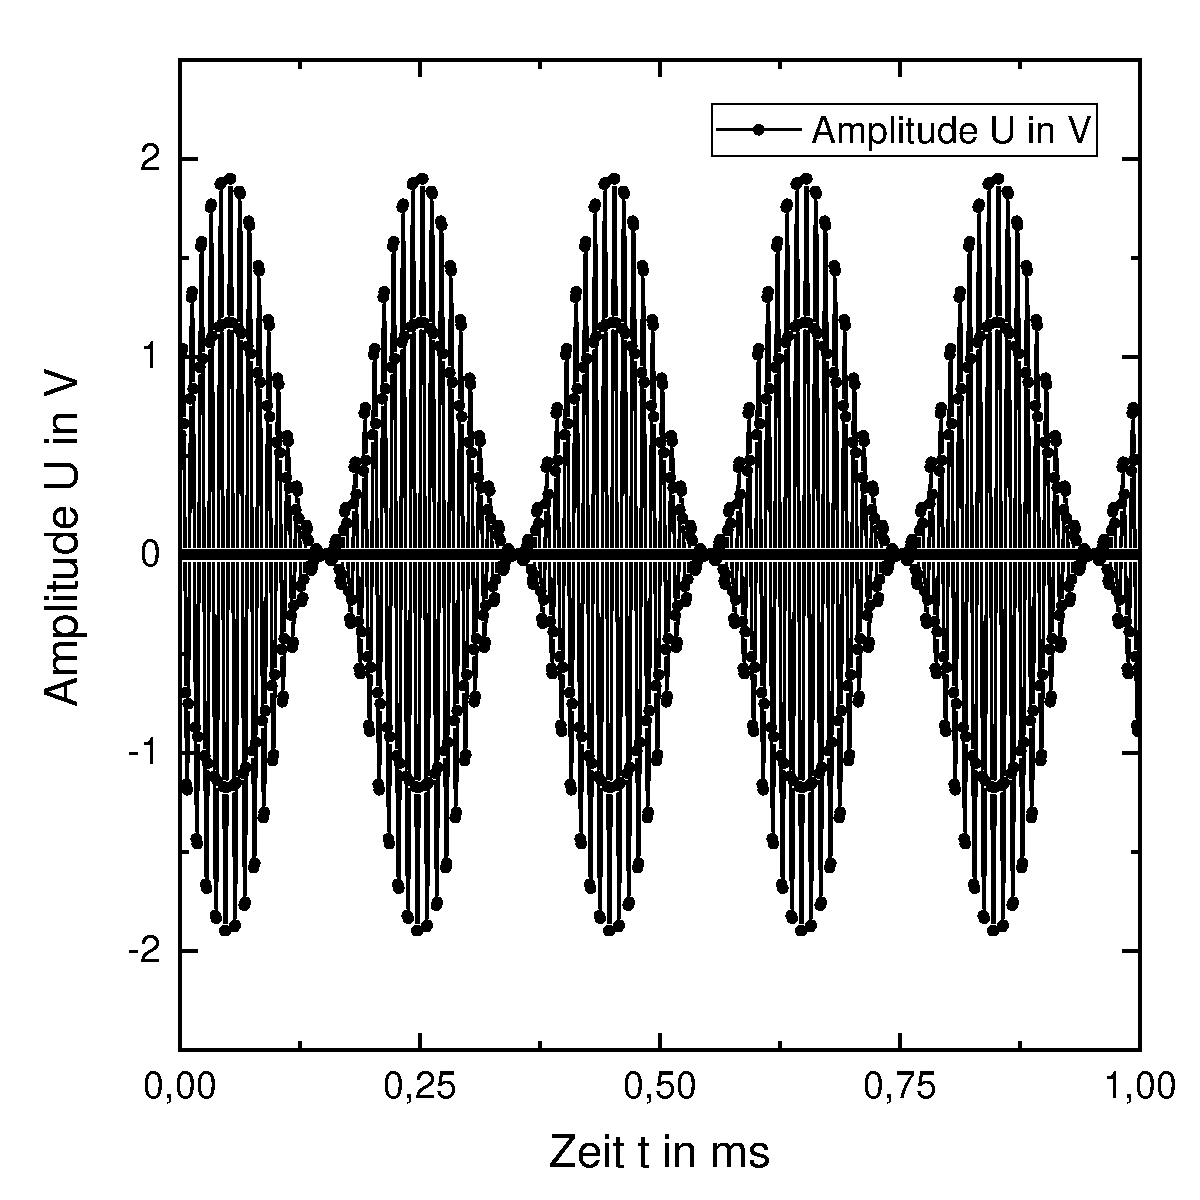
\includegraphics[width=\textwidth]{Bilder/AM2_additiv_Zeit.pdf}
    \end{subfigure}
    \begin{subfigure}{0.45\textwidth}
        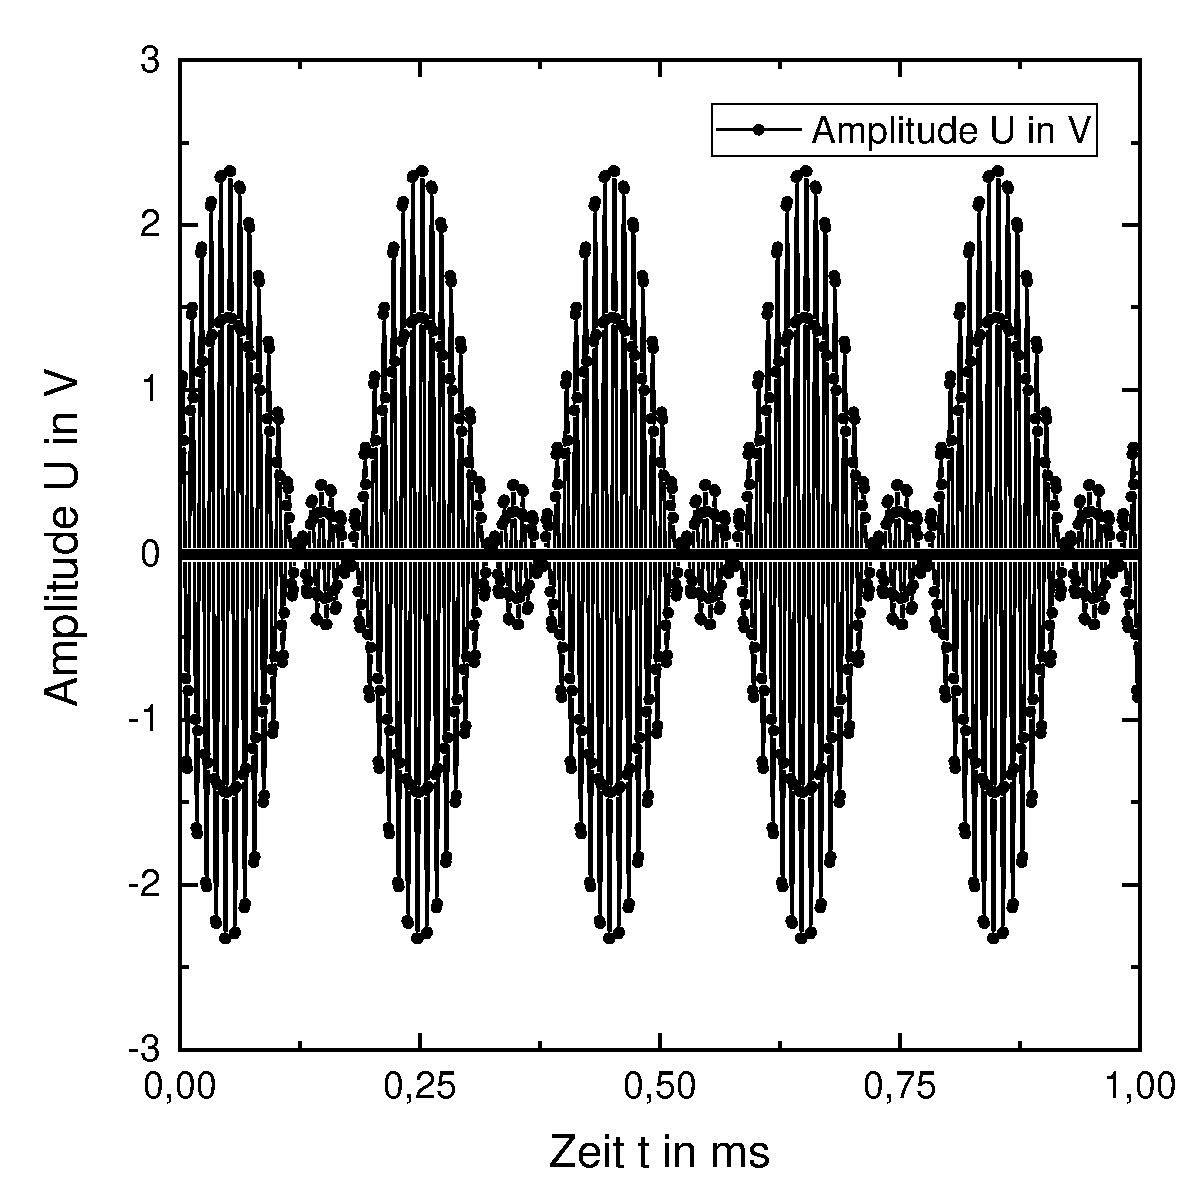
\includegraphics[width=\textwidth]{Bilder/AM3_additiv_Zeit.pdf}
    \end{subfigure}
    \caption{Veränderung des Modulationsgrades bei der additiven Amplitudenmodulation. Links wurde $U_\text{N} = \SI{1}{\volt}$ gewählt, was einem Modulationsgrad von $M = 1$ entspricht. Im rechten Bild war $U_\text{N} = \SI{1,45}{\volt}$ mit Modulationsgrad $M = 1,45$.}
    \label{fig:AM2_additiv}
\end{figure}\\
Wird die Amplitude des Nutzsignals größer als die des Trägers, dann ergibt sich ein Modulationsgrad $M > 1$ und es treten weitere Schwingungsbäuche auf. Abbildung~\ref{fig:AM2_additiv} zeigt den zeitlichen Verlauf einer solchen Schwingung. Eine solche Modulation sollte allerdings immer vermieden werden, da es durch die zusätzlichen Schwingungsbäuche zu einer Fehlinterpretation der auftretenden Frequenzen kommen kann.
\FloatBarrier
\newpage
\paragraph{Multiplikative Amplitudenmodulation}$~$\\
Weiterhin wurde noch eine multiplikative Amplitudenmodulation simuliert. Analog zu den vorherigen Simulationen wurde die Nutzfrequenz $ = \SI{5}{\kilo\hertz}$ und Trägerfrequenz $\nu_\text{T} = \SI{100}{\kilo\hertz}$ gewählt, siehe Abbildung~\ref{fig:AM1_multiplikativ}.
\begin{figure}[htp]
    \centering
    \begin{subfigure}{0.45\textwidth}
        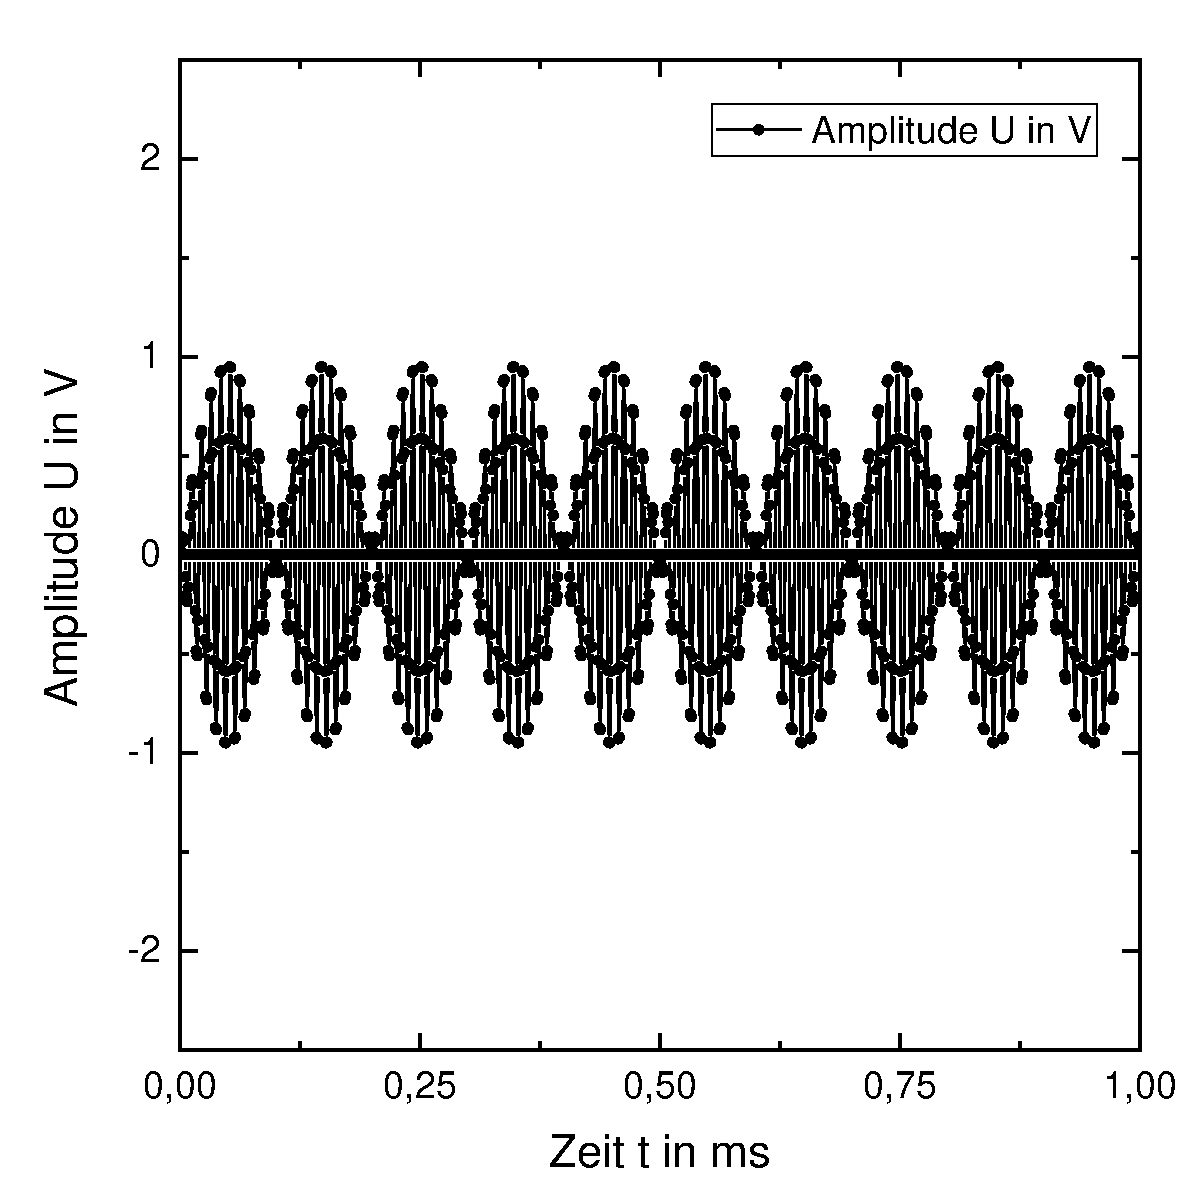
\includegraphics[width=\textwidth]{Bilder/AM1_mult_Zeit.pdf}
    \end{subfigure}
    \begin{subfigure}{0.45\textwidth}
        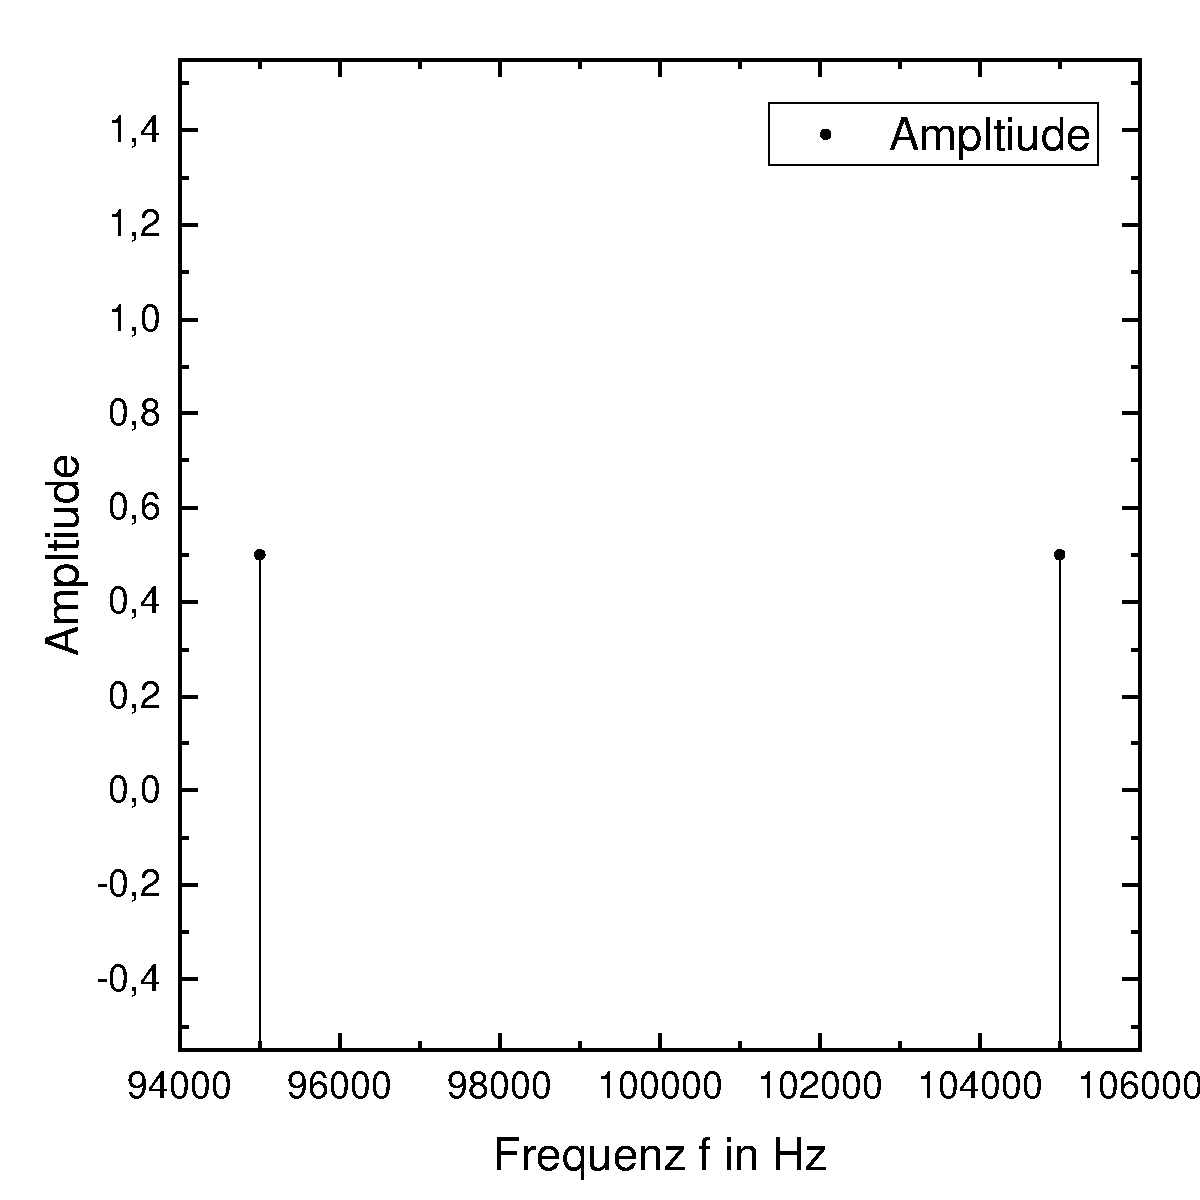
\includegraphics[width=\textwidth]{Bilder/AM1_mult_Frequenz.pdf}
    \end{subfigure}
    \caption{Zeitverlauf und Frequenzspektrum der multiplikativ amplitudenmodulierten Signale nach Formel \eqref{eqn:AM1_multiplikativ}. Es wurde eine Amplitude von $U_\text{N} = U_\text{T} = \SI{1}{\volt}$ gewählt.}
    \label{fig:AM1_multiplikativ}
\end{figure}\\
Bei der Analyse der Frequenzbereichs fällt auf, dass die Trägerfrequenz verschwunden ist und nur noch die beiden Seitenbänder sichtbar sind.\\
Für einen besseren Vergleich mit der additiven Amplitudenmodulation wurden ebenfalls die Amplituden des Nutzsignals auf $U_\text{N} = \SI{0,4}{\volt}$ (Abbildung~\ref{fig:AM2_multiplikativ} links) und auf $U_\text{N} = \SI{1,45}{\volt}$ (Abbildung~\ref{fig:AM2_multiplikativ} rechts) gesetzt.
\begin{figure}[htp]
    \centering
    \begin{subfigure}{0.45\textwidth}
        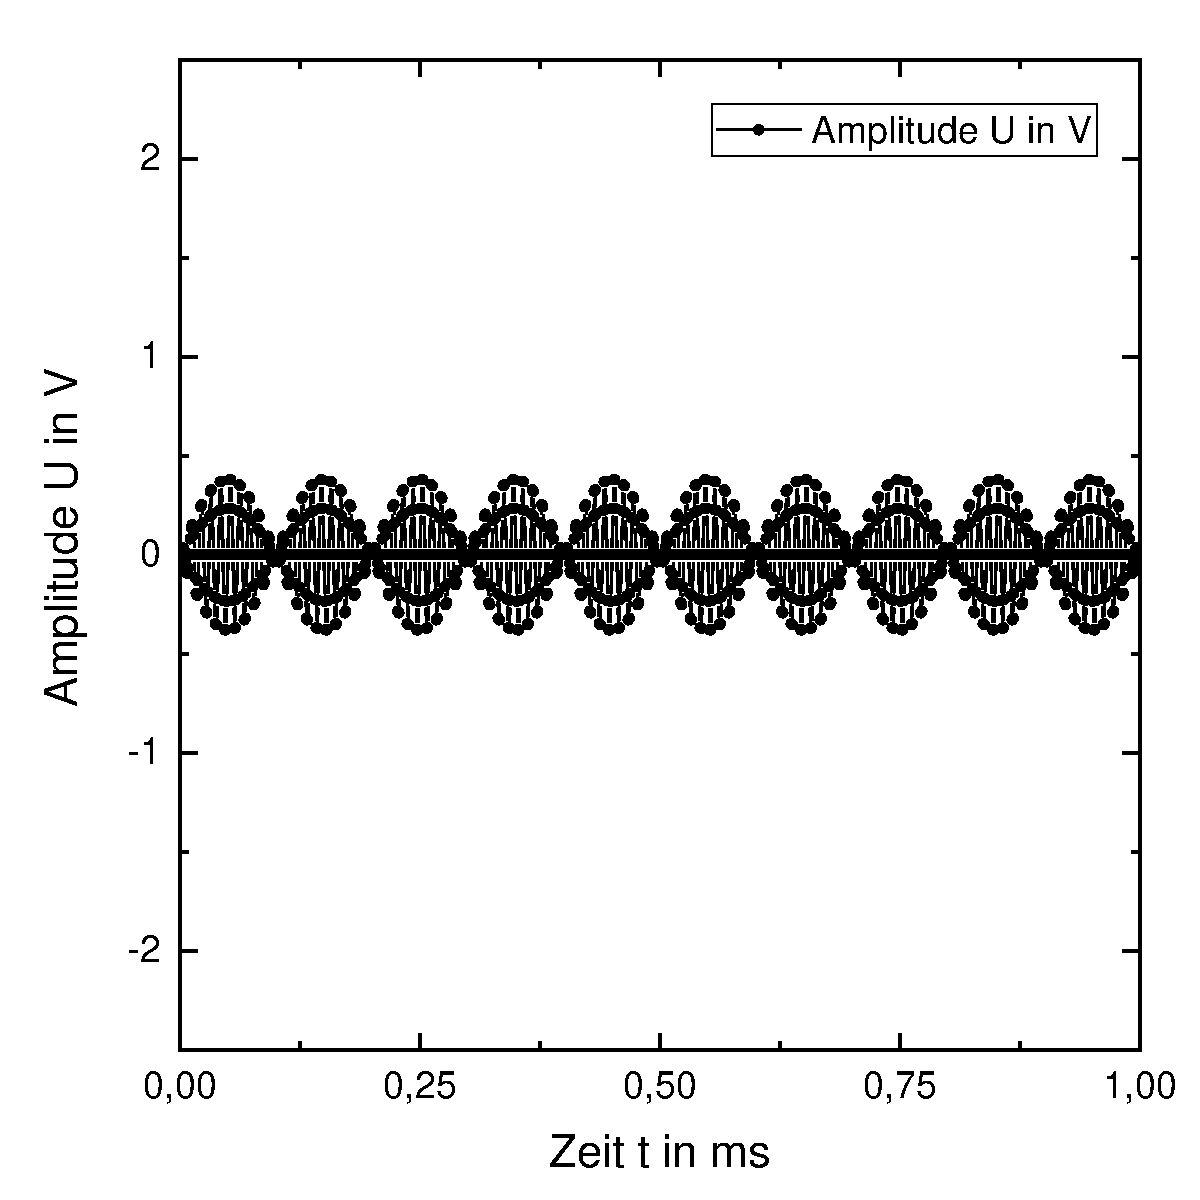
\includegraphics[width=\textwidth]{Bilder/AM2_mult_Zeit.pdf}
    \end{subfigure}
    \begin{subfigure}{0.45\textwidth}
        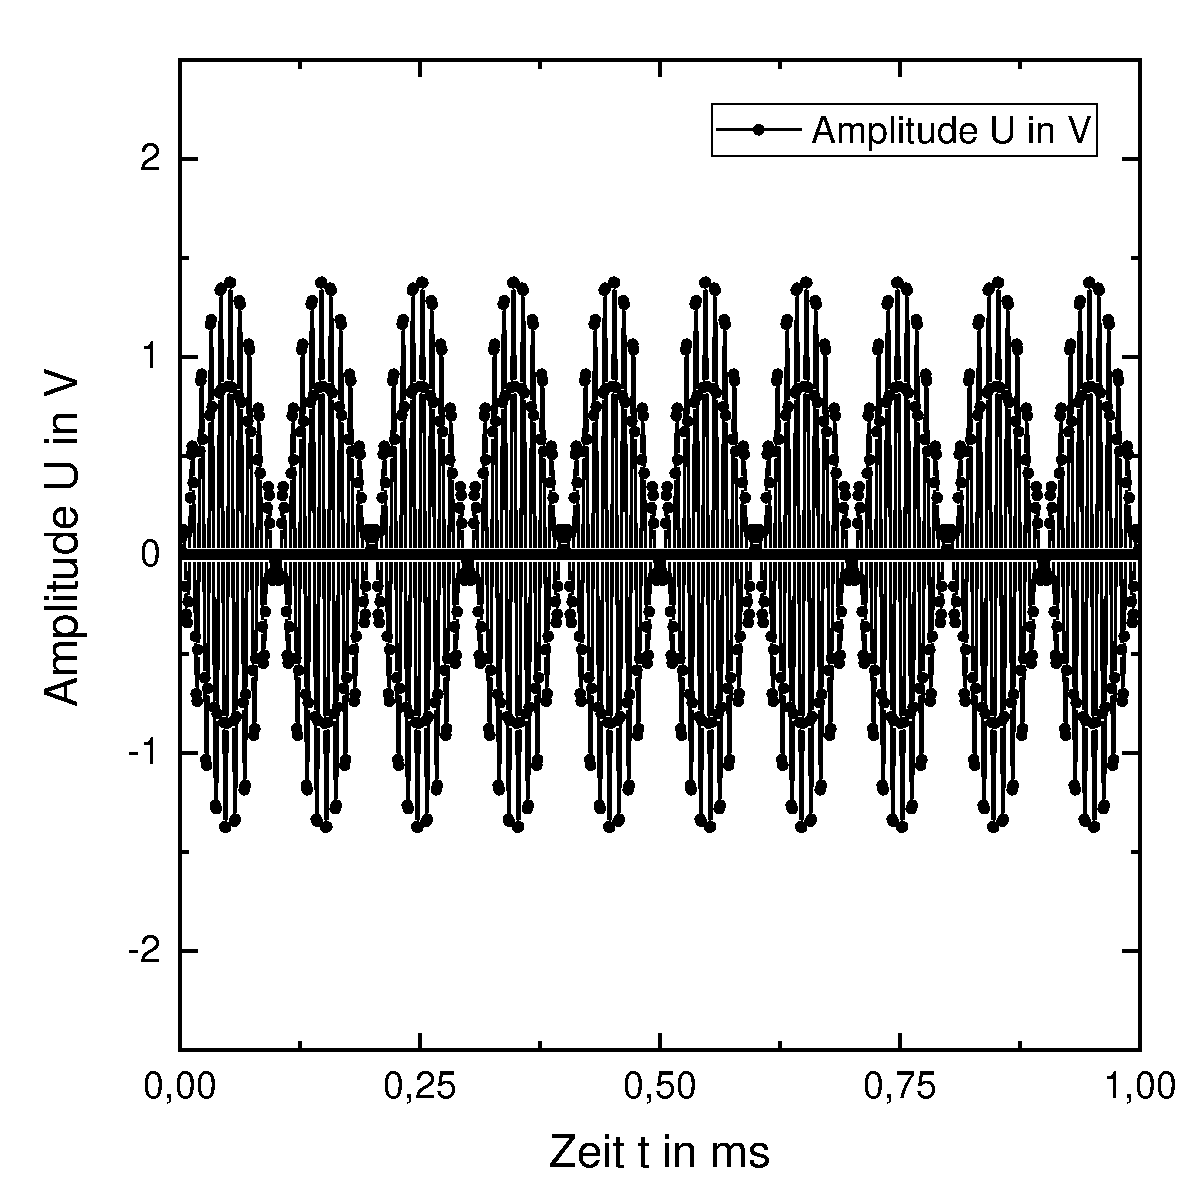
\includegraphics[width=\textwidth]{Bilder/AM3_mult_Zeit.pdf}
    \end{subfigure}
    \caption{Veränderung der Amplitude der multiplikativen Amplitudenmodulation bei Änderung der Amplitude des Nutzsignals.}
    \label{fig:AM2_multiplikativ}
\end{figure}\\
Es zeigt sich, die einhüllende Kurve der Modulation unabhängig von der Amplitude des Nutzsignals immer eine Nullstelle aufweist.
\FloatBarrier
\subsubsection{Amplitudenmodulation im Experiment}
Nun wurde die Amplitudenmodulation experimentell durchgeführt. Dabei wurde eine Nutzfrequenz von $\nu_\text{N} = \SI{100}{\kilo\hertz}$ und eine Trägerfrequenz von $\nu_\text{T} = \SI{100}{\mega\hertz}$ additiv überlagert. Dies wurde mithilfe einer Modulationsbox realisiert, deren Schaltplan in Abbildung~\ref{fig:AM_Modulator} dargestellt ist.
\begin{figure}[htp]
  \centering
  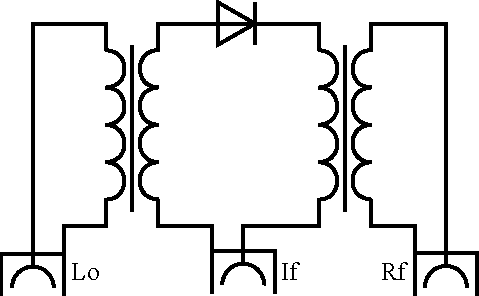
\includegraphics{Schaltungen/AM-Modulator.pdf}
  \caption{Schaltplan des im Versuch verwendeten AM-Modulators.}
  \label{fig:AM_Modulator}
\end{figure}\\
Das Zeitbild wurde an einem analogen Oszilloskop dargestellt, weil das \textit{HP 54845A} nicht gleichzeitig auf diese beiden unterschiedlichen Frequenzen triggern konnte, um ein stabiles Bild zu erzeugen. Da auch hier keine Möglichkeit zur Speicherung der Daten vorhanden war, sind die folgenden Verläufe als Photo dargestellt.
\begin{figure}[htp]
    \centering
    \begin{subfigure}{0.45\textwidth}
        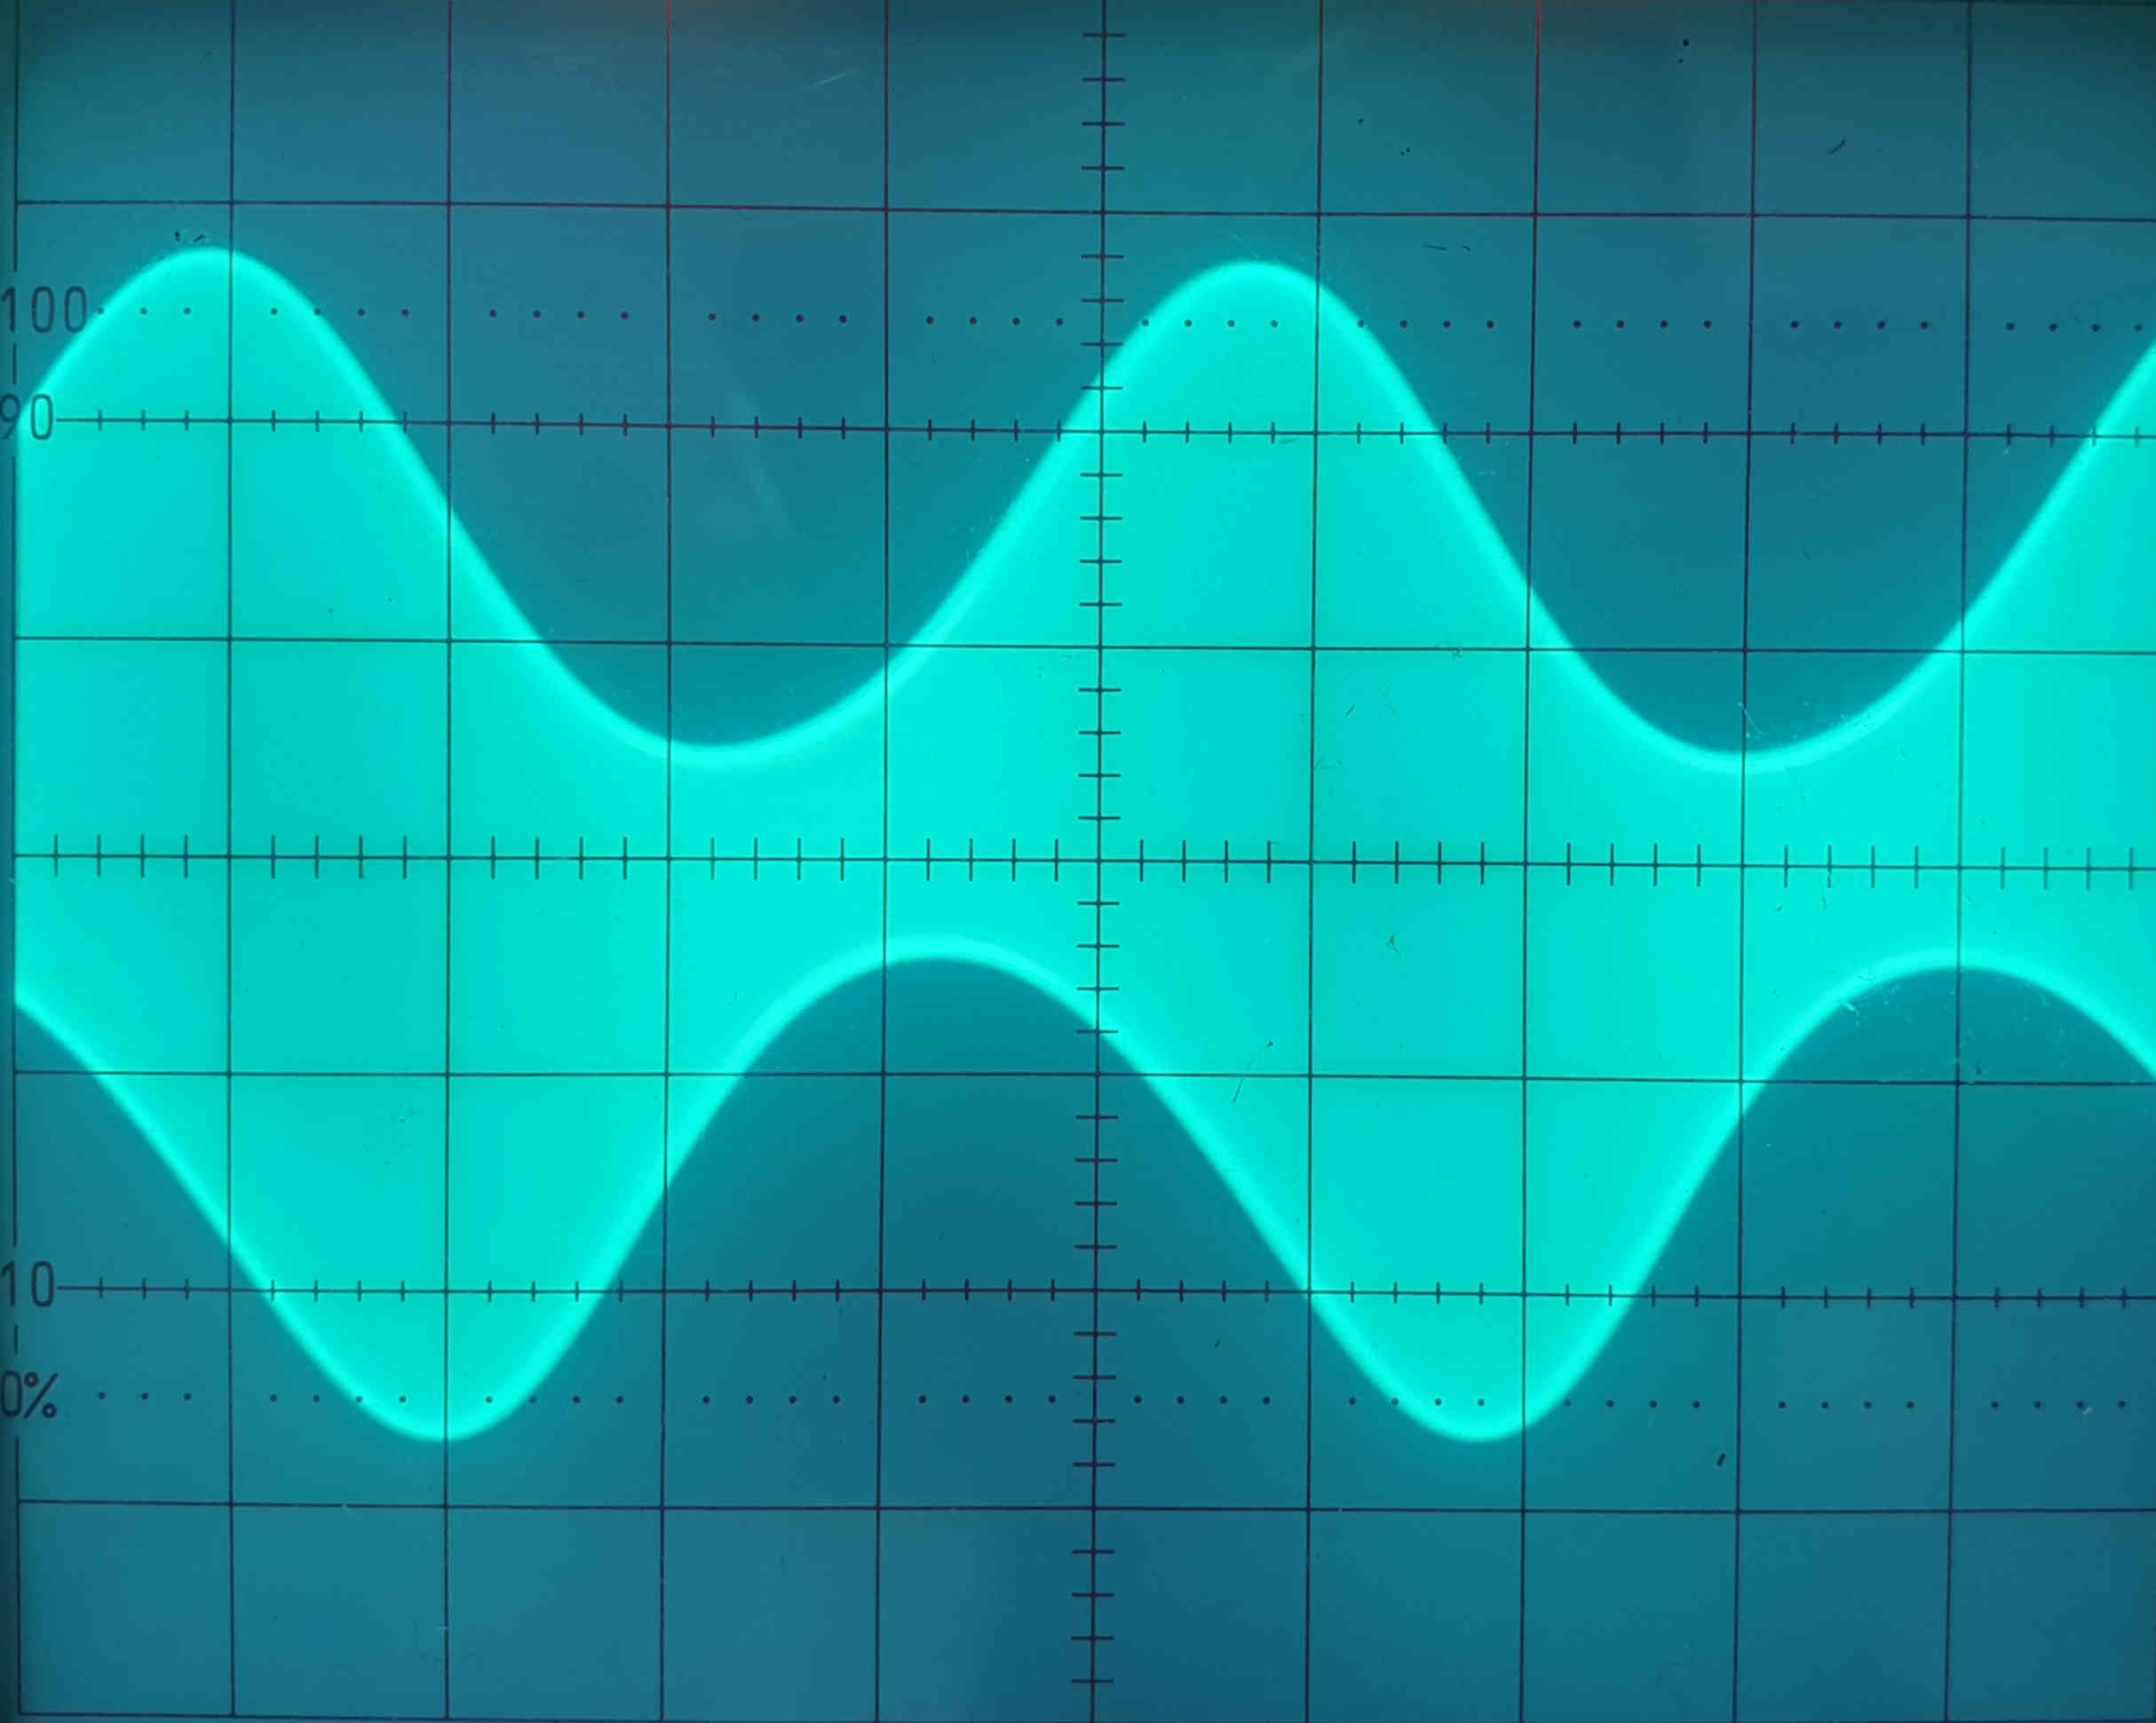
\includegraphics[width=\textwidth]{Bilder/AM_400mV_Amplitude.jpg}
        \caption{Zeitverlauf}
    \end{subfigure}\hspace{1cm}
    \begin{subfigure}{0.45\textwidth}
        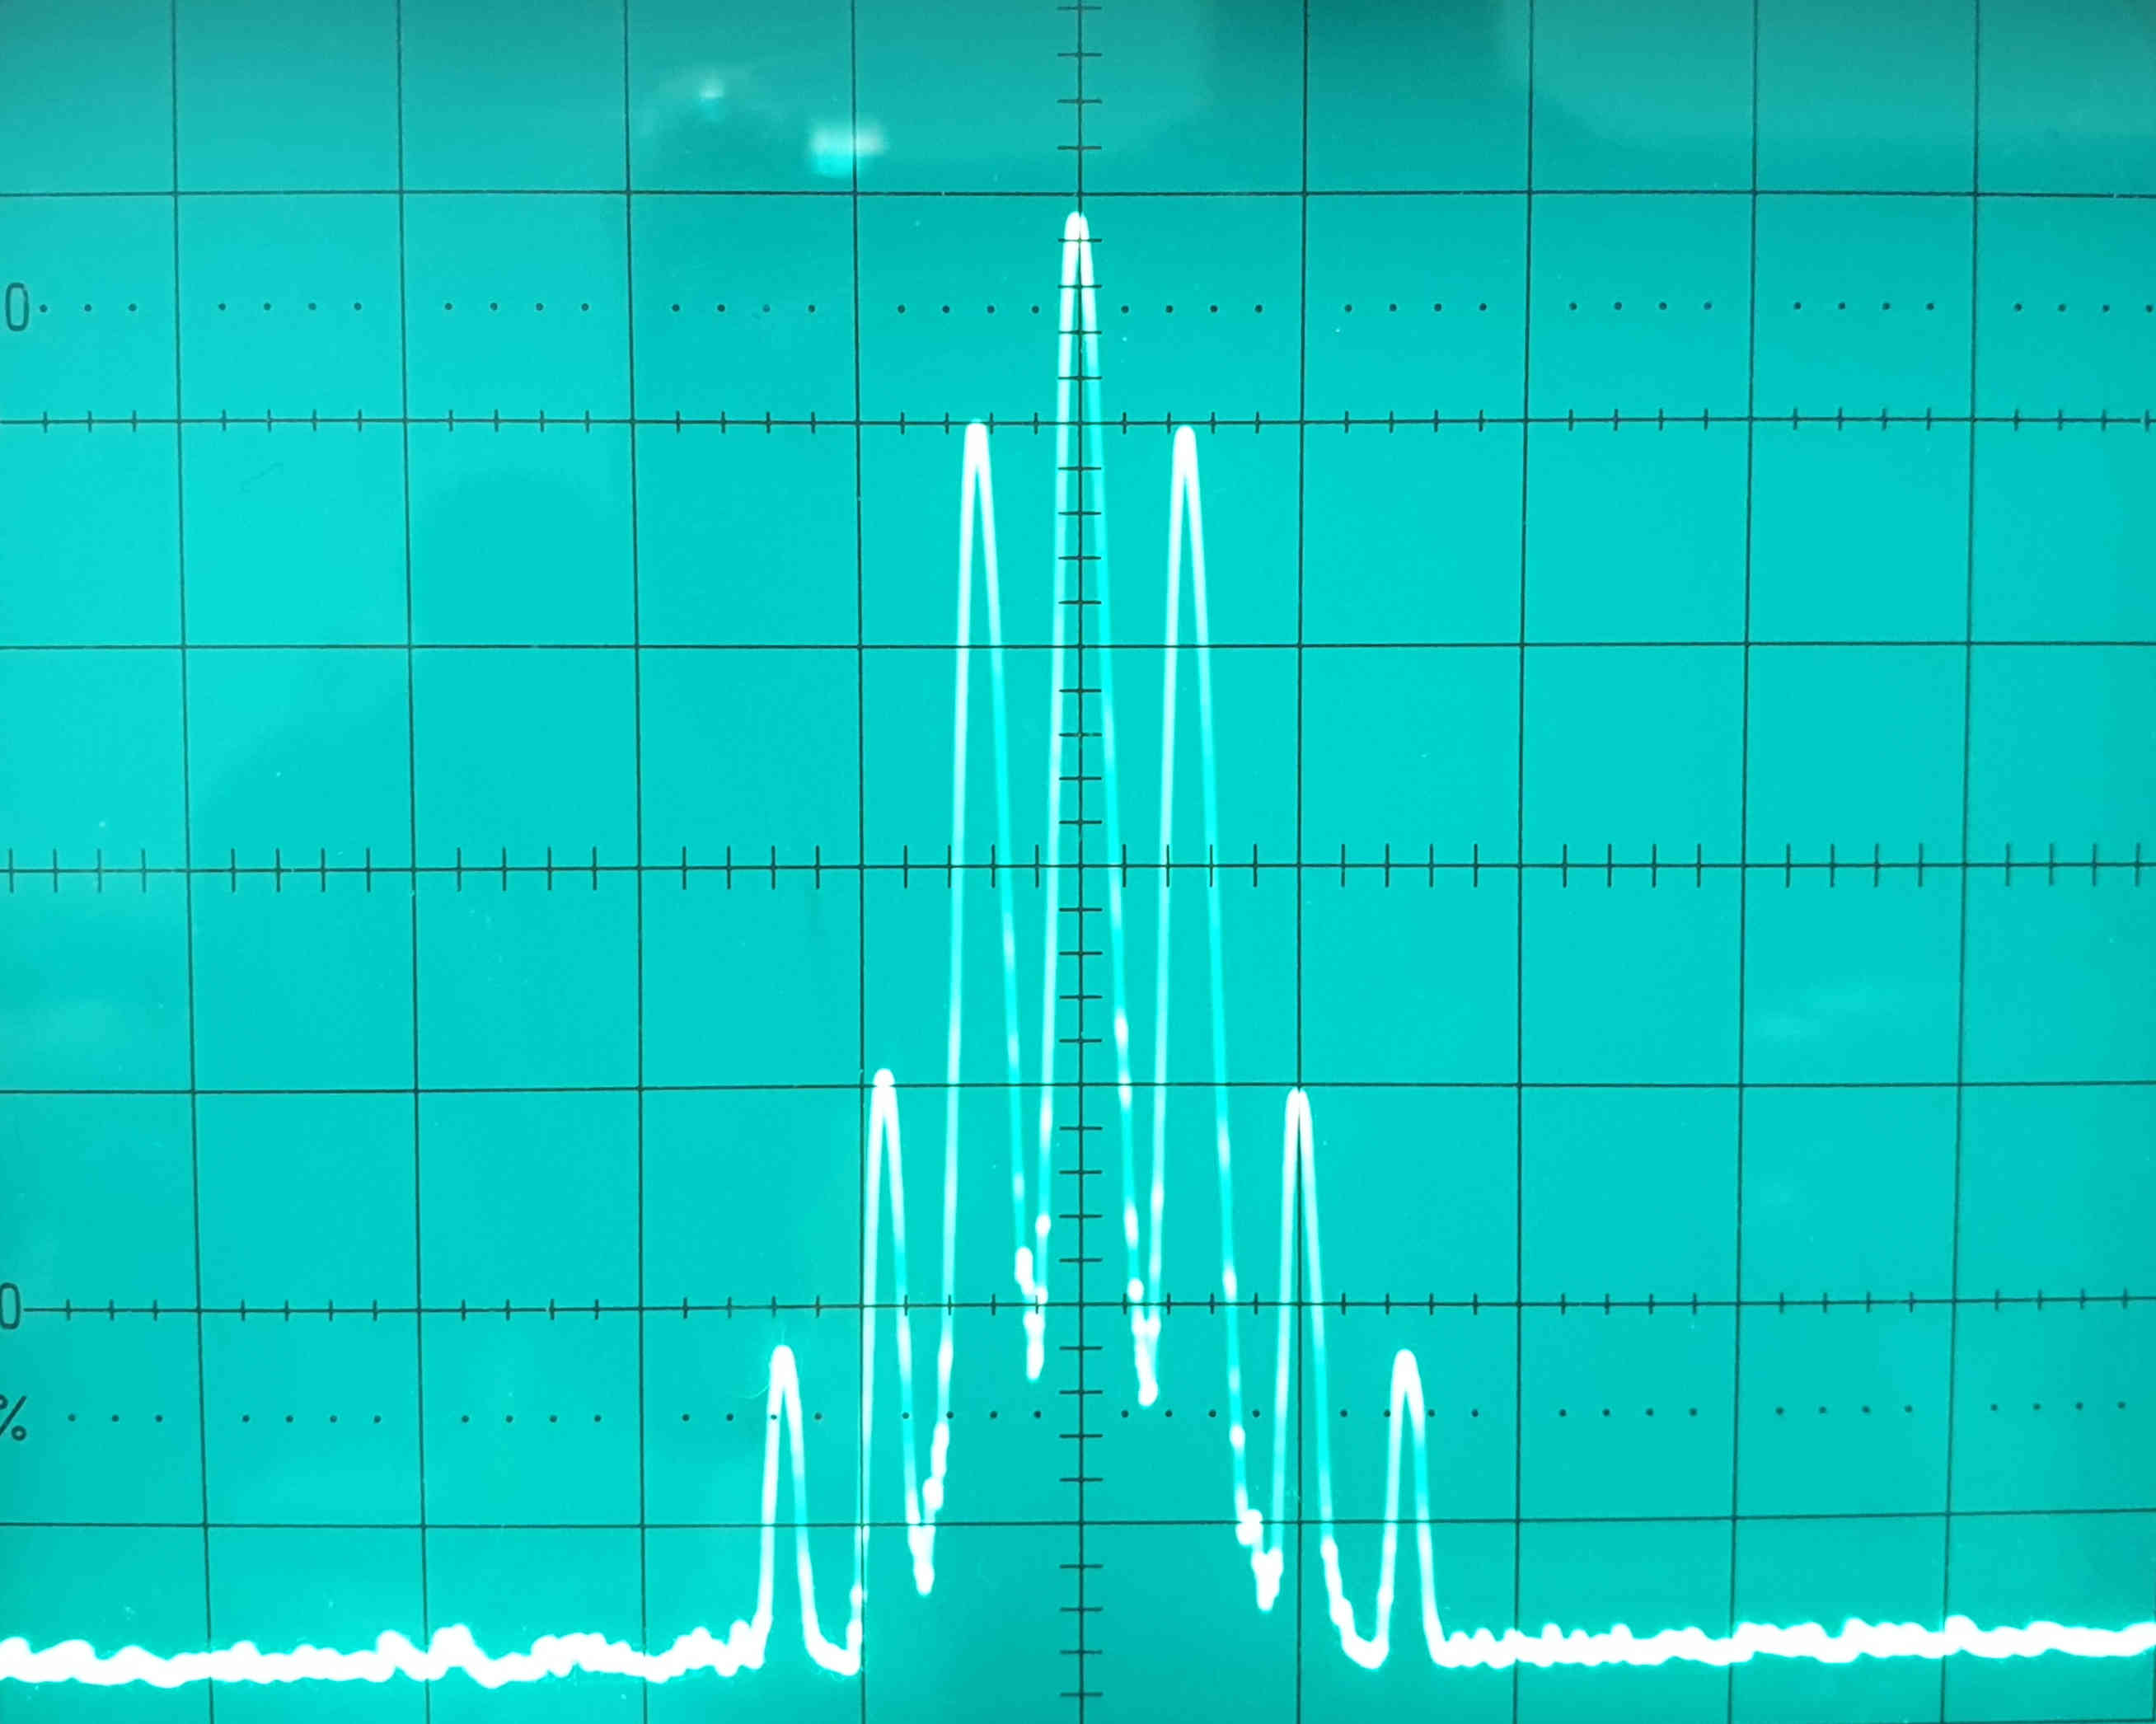
\includegraphics[width=\textwidth]{Bilder/AM_400mV_Frequenz.jpg}
        \caption{Frequenzverlauf}
    \end{subfigure}
    \caption{Additiv amplitudenmoduliertes Signal mit $\nu_\text{N} = \SI{100}{\kilo\hertz}$ und $\nu_\text{T} = \SI{100}{\mega\hertz}$ und einer Amplitude des Nutzsignals von $U_N = \SI{400}{\milli\volt_\text{PP}}$.}
    \label{fig:Modulation_400mV}
\end{figure}\\
Das Trägersignal wurde mit einer effektiven Spannung von $\SI{1}{\volt}$ generiert und mit einem $10:1$ Element abgeschwächt. Als Amplitude des Nutzsignals wurde $U_N = \SI{400}{\milli\volt_\text{PP}}$ eingestellt. Im Zeitverlauf sieht das modulierte Signal verschoben aus, die Minima und Maxima der Hüllkurve sind zueinander verschoben.\\
Das Frequenzspektrum wurde an einem analogen Frequenzspektrographen mit logarithmischer Ordinate dargestellt. Ein Kästchen entlang der Ordinate beschreibt eine Intensitätsabschwächung von $\SI{10}{\deci\bel} \approx 0,32$. Die Amplituden der ersten Seitenbänder entsprechen demnach etwa nur $\SI{30}{\percent}$ der Amplitude der Trägerfrequenz. Im Unterschied zur Simulation treten hier Seitenbänder höherer Ordnung $\omega_\text{T}\pm n\cdot \omega_\text{N}$ auf. Diese sind aber um 40 bzw. $\SI{50}{\deci\bel}$ gegenüber der Trägerfrequenz abgeschwächt, was einer Abschwächung um Faktor 100 bzw. 300. Die Nebenfrequenzen treten auf, weil die Kennlinien der zur Modulation verwendeten Dioden nicht exakt quadratisch sind.\\ %ToDo mehr dazu
Weiterhin wurde die Modulation mit gleichen Frequenzen von Signal und Träger aber einer anderen Amplitude $U_\text{N} = \SI{800}{\milli\volt}$ wiederholt. Das Ergebnis zeigt Abbildung~\ref{fig:Modulation_800mV}
\begin{figure}[htp]
    \centering
    \begin{subfigure}{0.45\textwidth}
        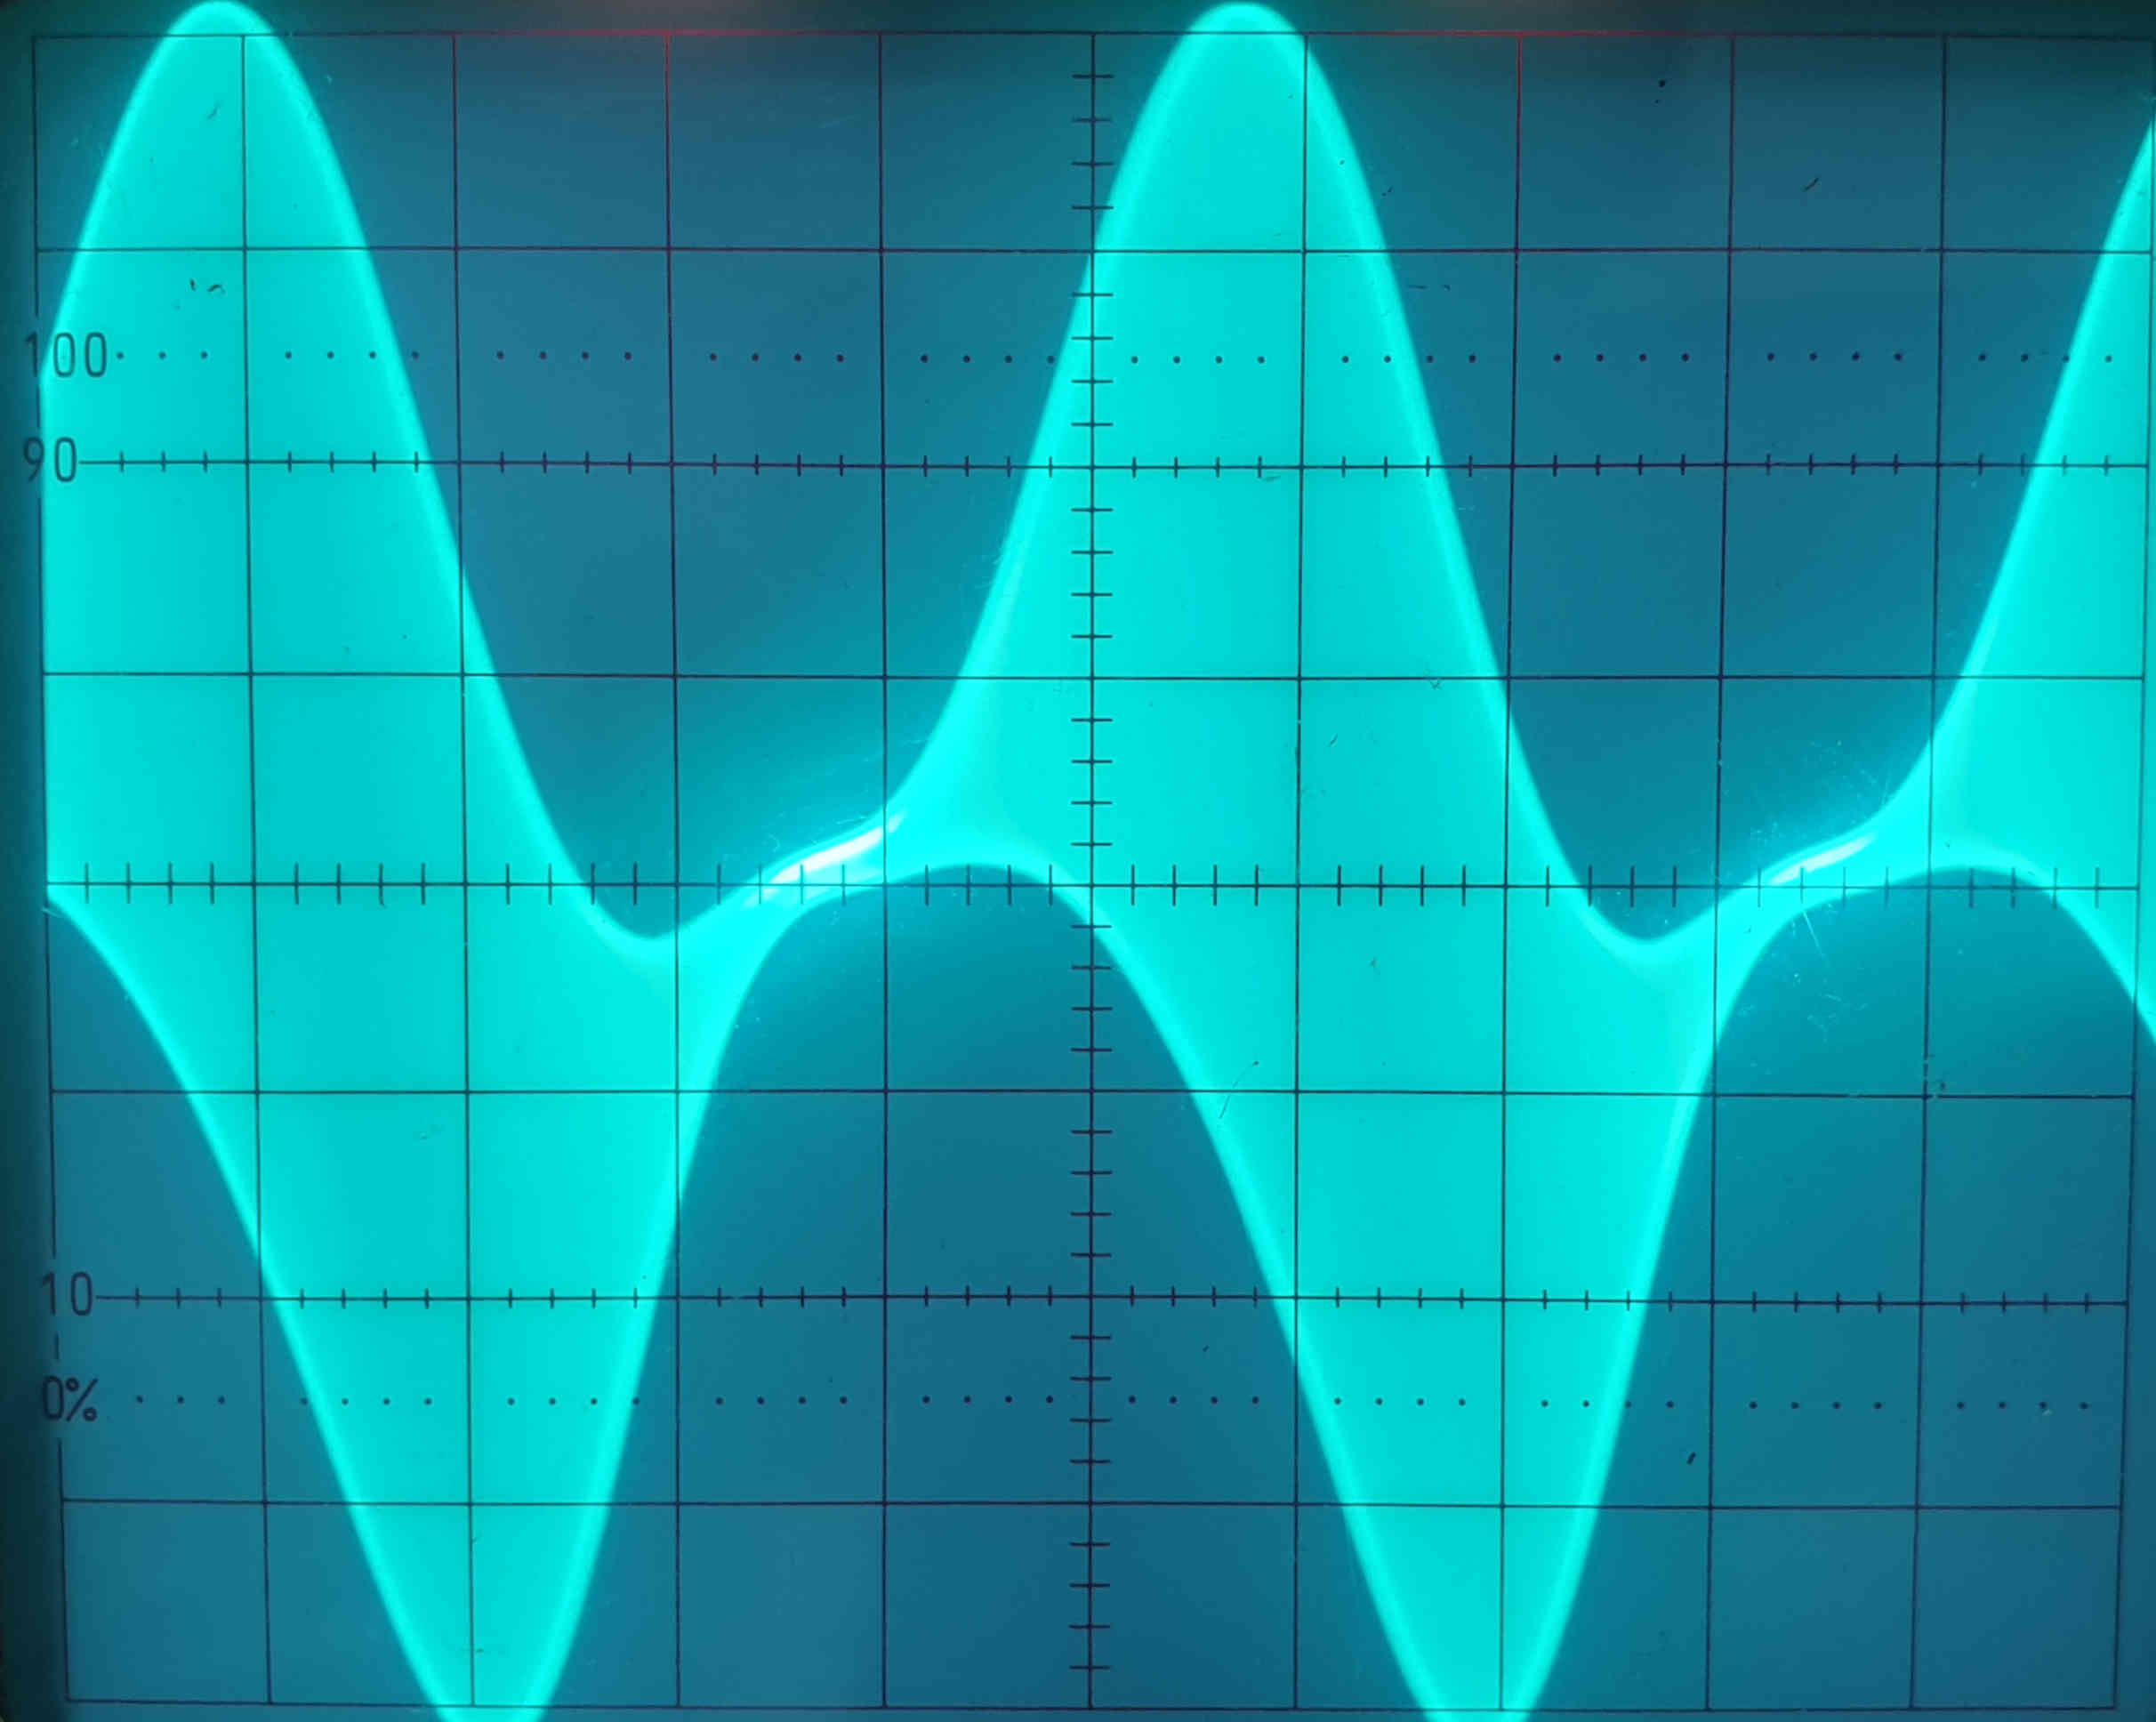
\includegraphics[width=\textwidth]{Bilder/AM_800mV_Amplitude.jpg}
        \caption{Zeitverlauf}
    \end{subfigure}\hspace{1cm}
    \begin{subfigure}{0.45\textwidth}
        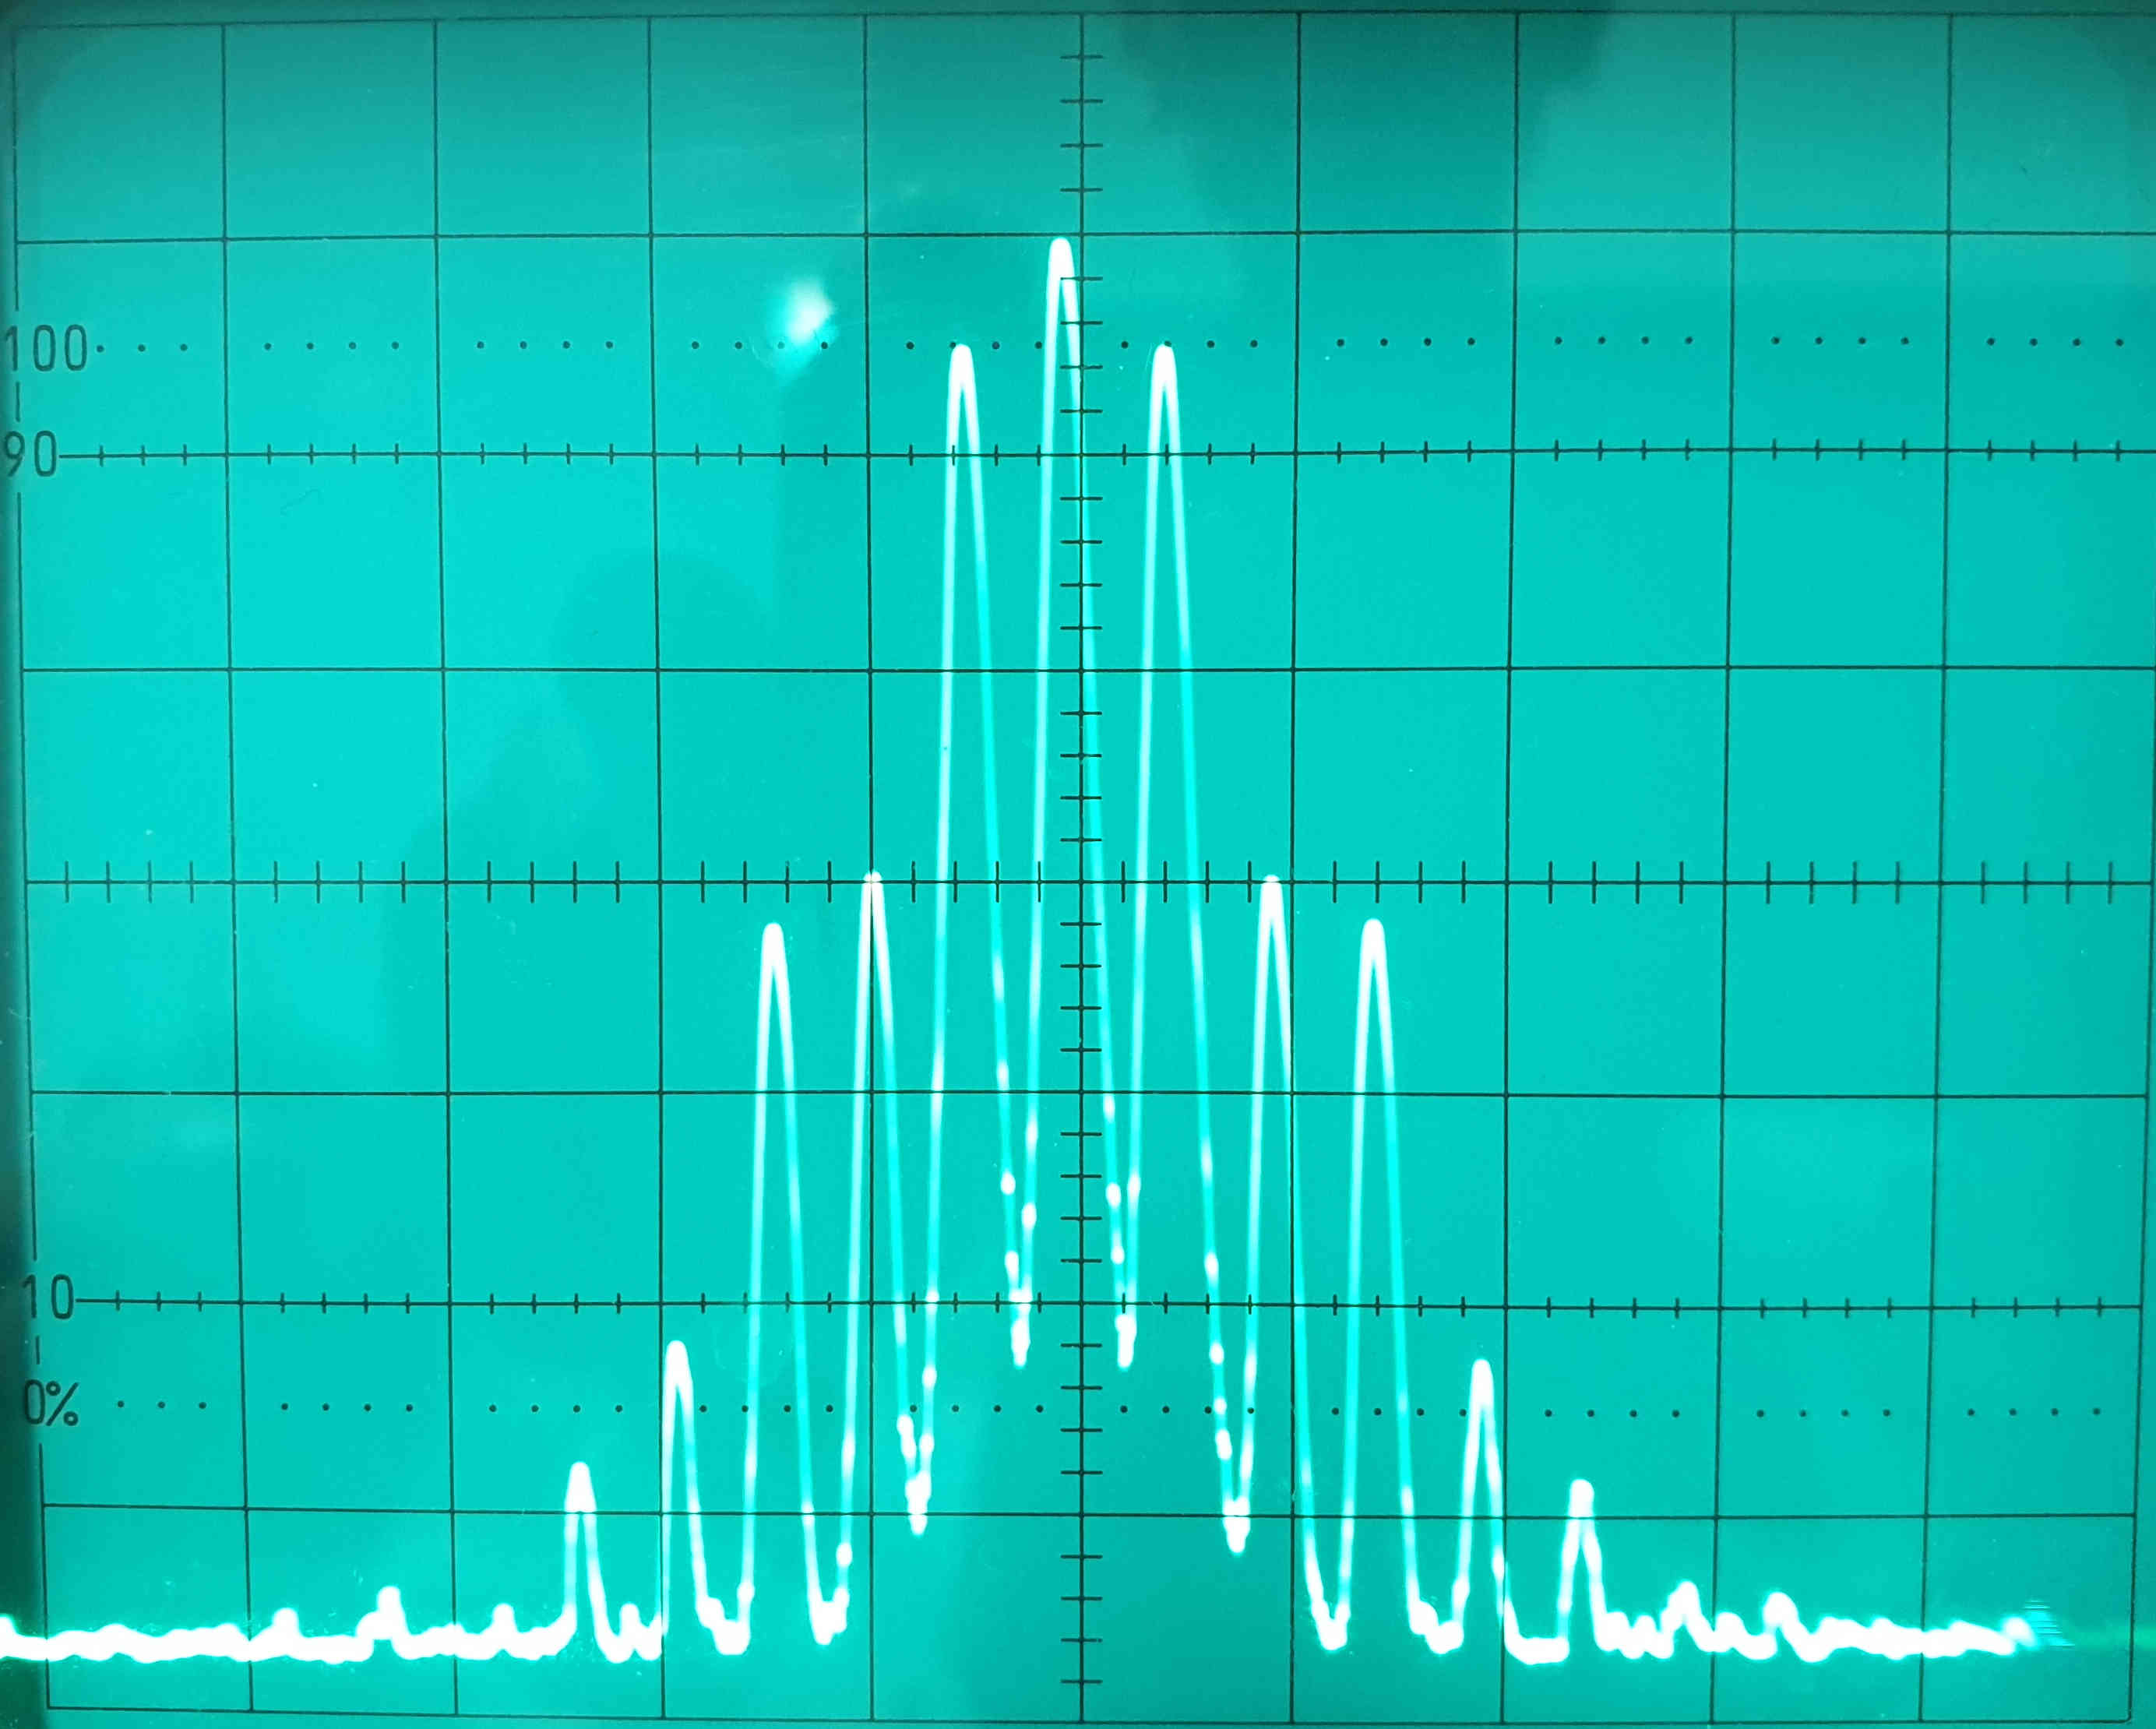
\includegraphics[width=\textwidth]{Bilder/AM_800mV_Frequenz.jpg}
        \caption{Frequenzverlauf}
    \end{subfigure}
    \caption{Additiv amplitudenmoduliertes Signal mit $\nu_\text{N} = \SI{100}{\kilo\hertz}$ und $\nu_\text{T} = \SI{100}{\mega\hertz}$ und einer Amplitude des Nutzsignals von $U_N = \SI{800}{\milli\volt_\text{PP}}$.}
    \label{fig:Modulation_800mV}
\end{figure}\\
Im Zeitverlauf ist der höhere Modulationsgrad gut erkennbar und kann als $M = 1$ abgeschätzt werden. Jedoch tritt weiterhin die Verschiebung der Einhüllenden Kurve auf. Im Frequenzspektrum sind die Seitenbänder wesentlich stärker ausgeprägt. Das erste Seitenband ist um $\SI{5}{\deci\bel}$ abgeschwächt, was einer Abschwächung von $\SI{50}{\percent}$ gegenüber der Trägerfrequenz entspricht. Dabei stimmt die Abschwächung mit dem erwarteten Ergebnis mit Modulationsgrad $M =1$ überein.
\subsection{Demodulation}
Die nach der im letzten Abschnitt behandelten Methode der Amplitudenmodulation werden nun über eine $\SI{25}{\metre}$ lange Koaxialleitung transportiert und anschließend demoduliert. Hierfür wurde eine Nutzfrequenz von $\nu_\text{N} =\SI{500}{\hertz}$ mit einem Träger von $\nu_\text{T}=\SI{100}{\mega\hertz}$ verwendet. Das Signal wurde zunächst mit einem analogen Oszilloskop im Zeitverlauf analysiert (Abbildung~\ref{fig:Demodulation} links) und am Frequenzspektrographen auf das Spektrum analysiert. Jedoch liegen die Seitenbänder mit $\nu_\text{T}\pm\SI{500}{\hertz}$ zu nah an der Trägerfrequenz, um sie am Spektrographen aufzulösen.
\begin{figure}[htp]
    \centering
    \begin{subfigure}{0.45\textwidth}
        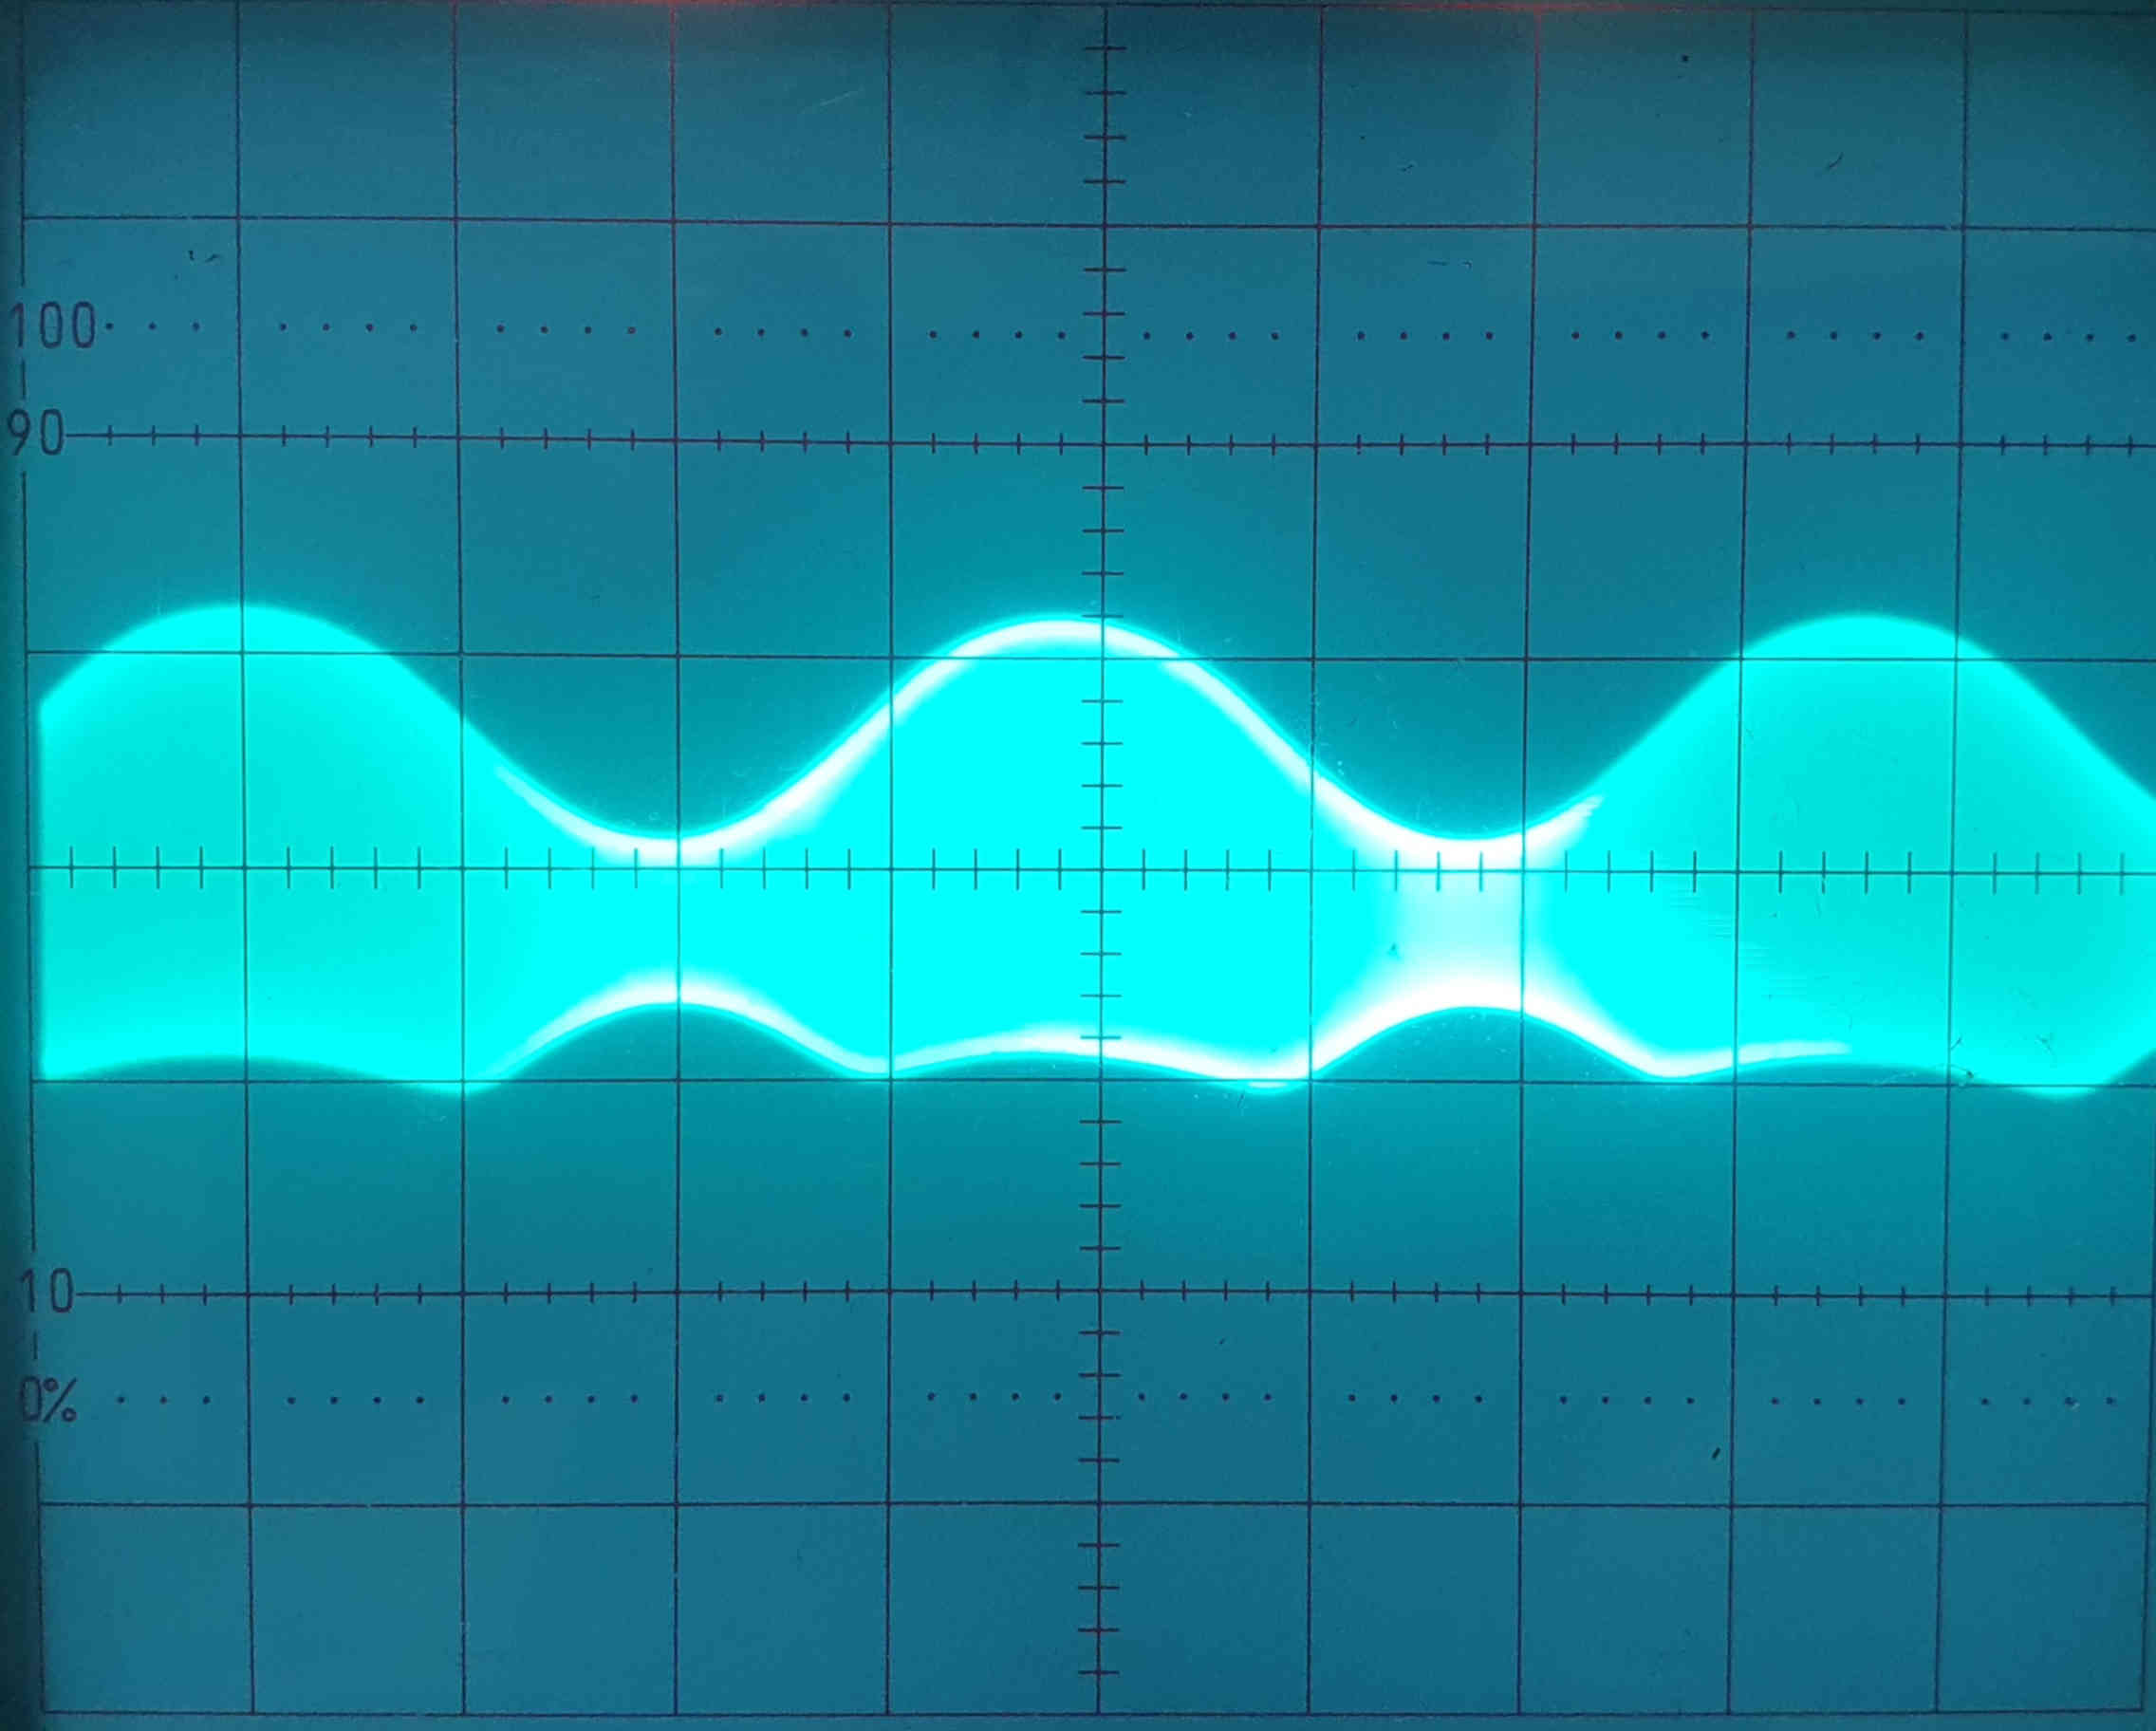
\includegraphics[width=\textwidth]{Bilder/AM_500Hz_200MHz.jpg}
        \caption{Moduliertes Signal}
    \end{subfigure}\hspace{1cm}
    \begin{subfigure}{0.45\textwidth}
        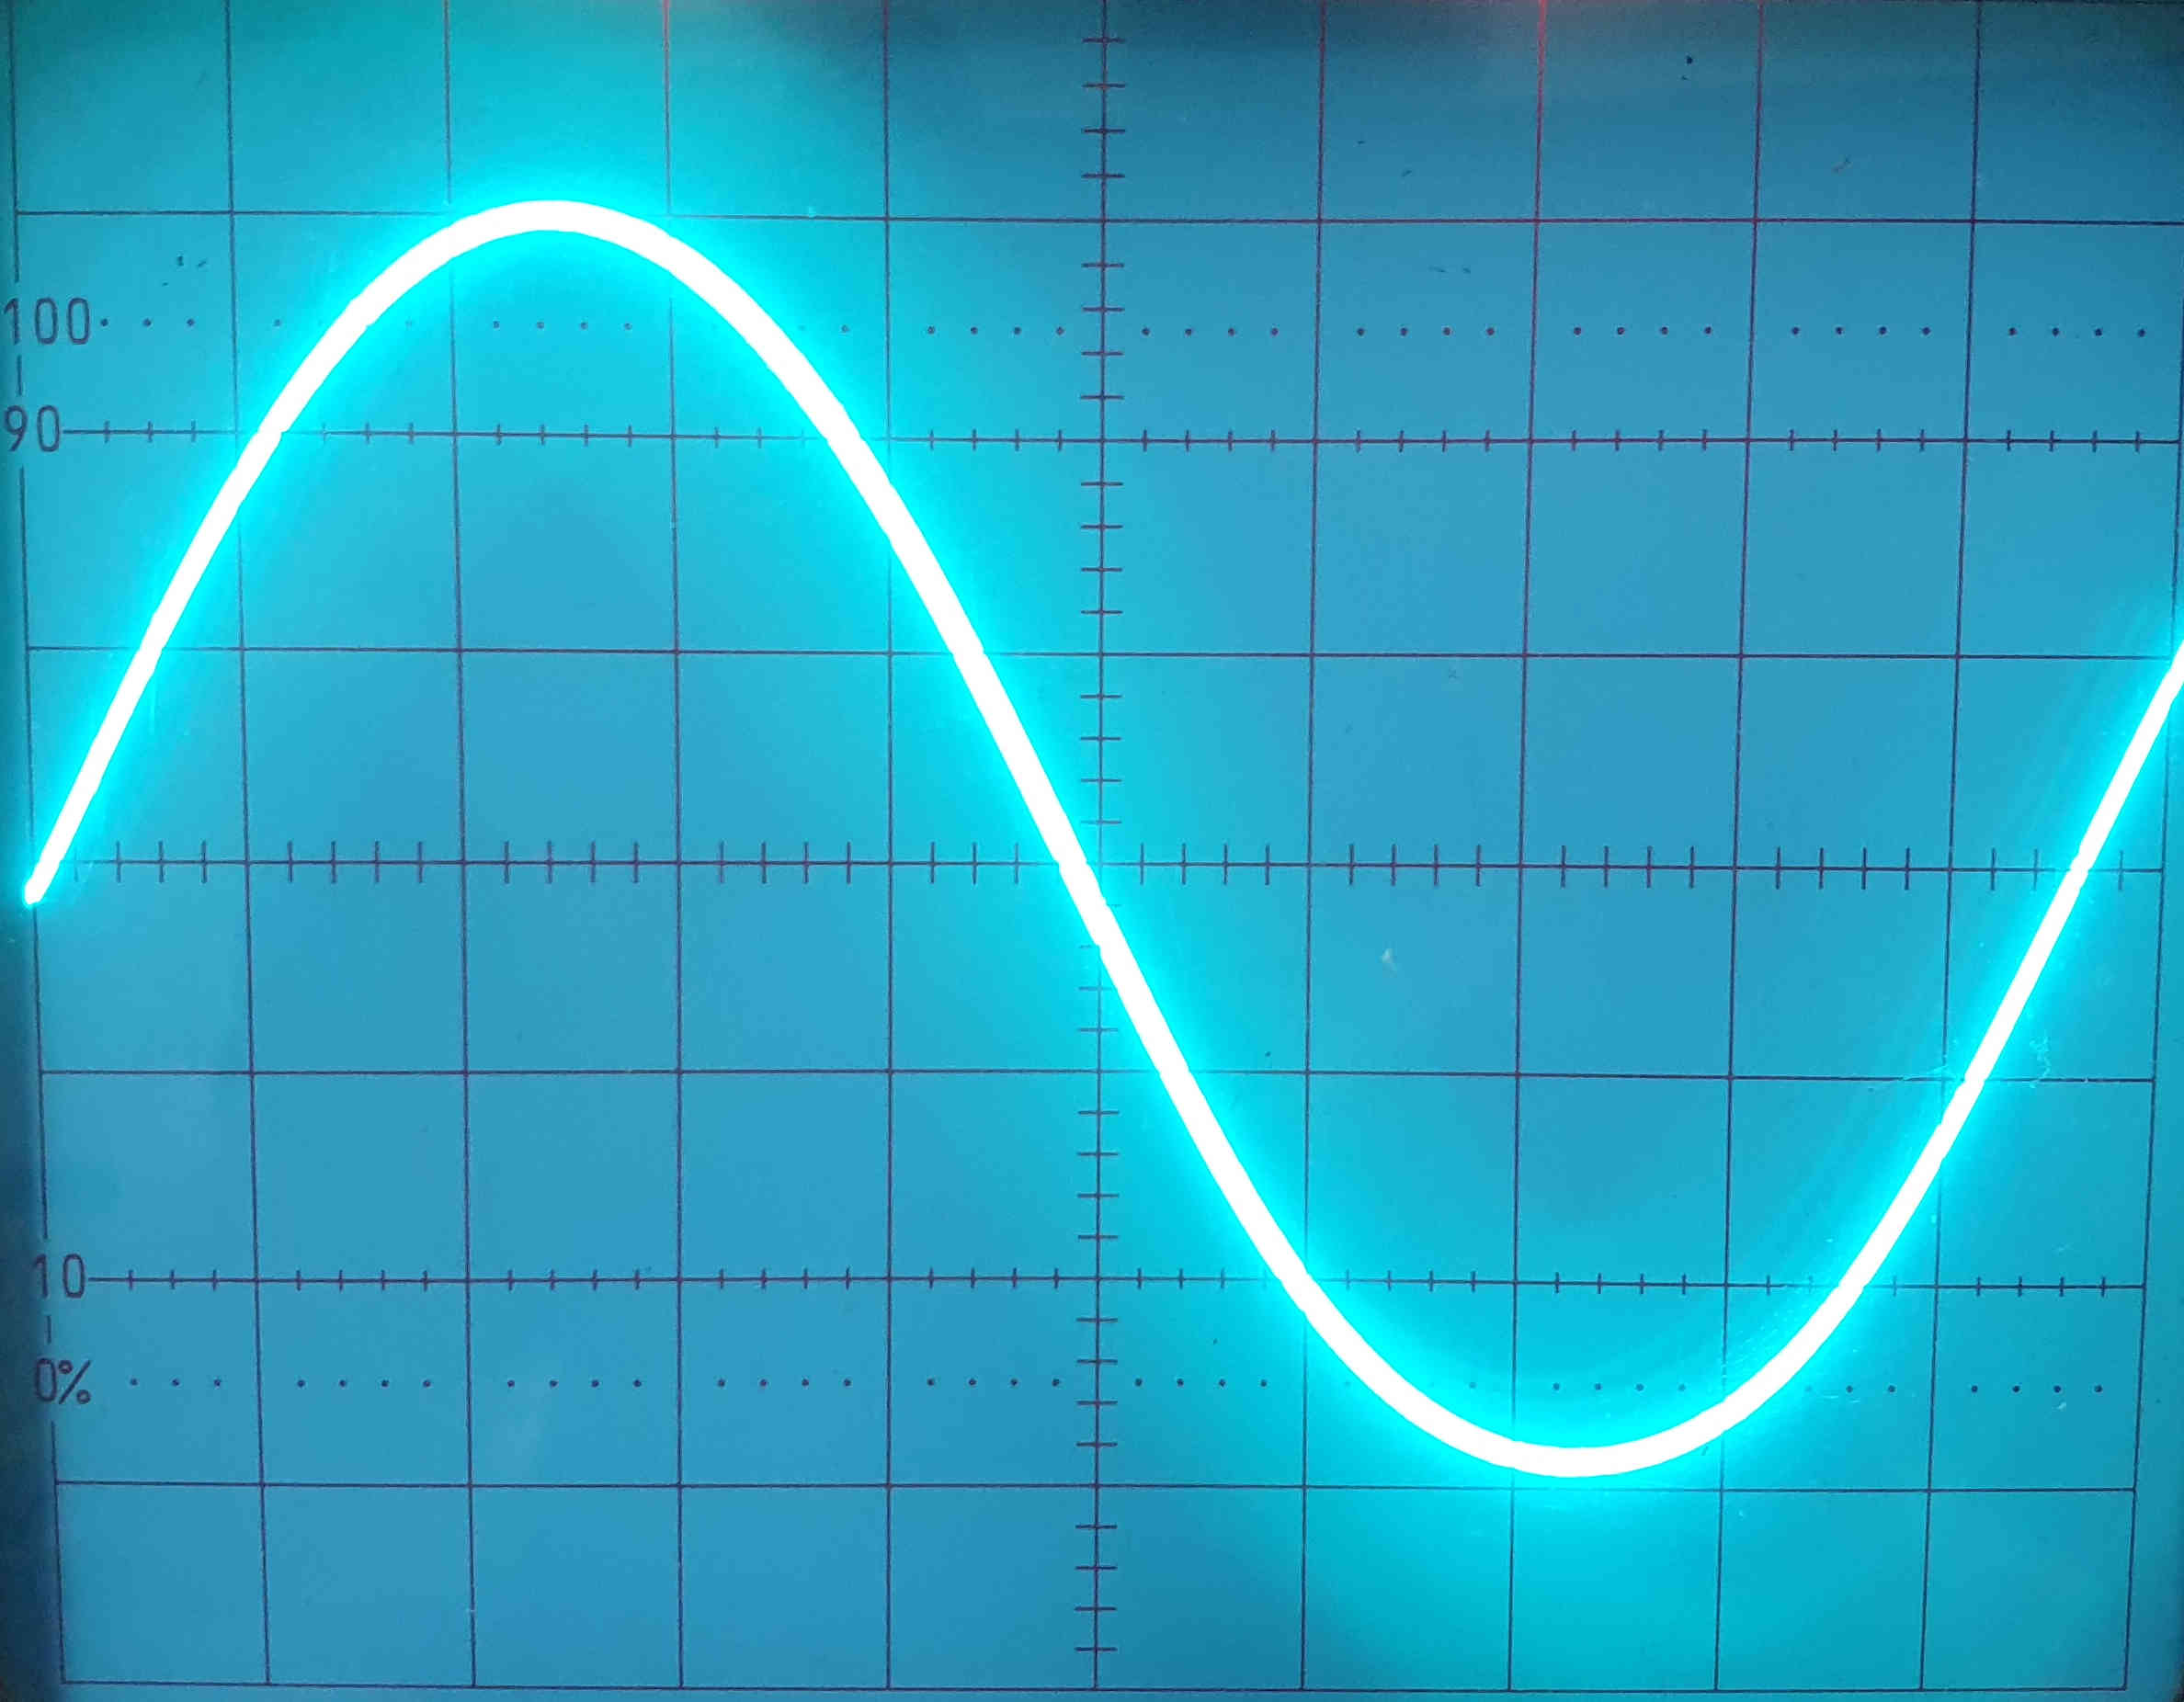
\includegraphics[width=\textwidth]{Bilder/AM_500Hz_demoduliert.jpg}
        \caption{Demoduliertes Signal}
    \end{subfigure}
    \caption{Additiv amplitudenmoduliertes Signal mit $\nu_\text{N} = \SI{500}{\hertz}$ und $\nu_\text{T} = \SI{200}{\mega\hertz}$ und anschließend demoduliertes Nutzsignal.}
    \label{fig:Demodulation}
\end{figure}\\
In Abbildung~\ref{fig:Demodulation} rechts ist der Zeitverlauf des demodulierten Signals dargestellt. Um ein stabiles Bild zu erhalten, wurde das Oszilloskop extern von einem Frequenzgenerator mit Rechteckimpulsen einer Frequenz von $\SI{500}{\hertz}$ getriggert.\\
Um die erhaltene Frequenz zu überprüfen, wurde aus dem Bild die Periodendauer abgelesen und die Frequenz berechnet. Dabei entsprach ein Kästchen auf dem Oszilloskop einer Zeit von $\SI{0,2}{\milli\second}$.
\begin{align}
  \nu &= \frac{1}{T} = \frac{1}{9,6\cdot \SI{0,2}{\milli\second}} = \SI{521}{\hertz}\\
  \Delta \nu &= \frac{\Delta T}{T^2} = \frac{0,2\cdot \SI{0,2}{\milli\second}}{(9,6\cdot \SI{0,2}{\milli\second})^2} = \SI{11}{\hertz}.
\end{align}
Die Signalfrequenz liegt nicht im Konfidenzintervall der Frequenzbestimmung von $\nu = \SI{521\pm 11}{\hertz}$. Dies lässt auf Fehler bei der Modulation schließen, denn bei Betrachtung von Abbildung~\ref{fig:Demodulation} links wird deutlich, dass die Modulation aufgrund der nicht exakt quadratischen Diodenkennlinie verzerrt wird. Fehler können auch bei der Demodulation an der Diode oder dem Glättungskondensator entstehen.

\subsection{Elektromagnetische Wellen im freien Raum}
Zunächst wird eine $\frac{\lambda}{2}$ Antenne auf \SI{200}{\mega\hertz} eingestellt. Dazu wird mit einer Rechnung die theoretische Länge mit dem idealen Verkürzungsfakor K = 0,98 berechnet:
\begin{align}
L = \frac{\lambda_\text{eff}}{2} = \frac{c_0 \cdot K}{2 \cdot f} = \frac{\SI{3e8}{\metre\per\second} \cdot 0,98}{2 \cdot \SI{200e8}{\hertz}}  = \SI{0,74}{\metre}.
\end{align}
Die tatsächliche Länge der Antenne wird dann durch systematisches Probieren ermittelt. Der oben errechnete Wert wird als Ausgangspunkt benutzt. Mit Hilfe des Reflektiometers wird das rücklaufende Signal beobachtet und in Abhängigkeit der eingestellten Länge bestimmt, bei welcher Frequenz dieses sein Minimum annimmt. Die Länge der Antenne wird solang verändert bis das Minimum der rücklaufenden Welle bei der gegebenen Frequenz vorliegt. Dies ist bei einer Länge von $L = \SI{73,3}{\centi\metre}$ der Fall. Dann gilt $U_\text{Rück, min} = \SI{19}{\milli\volt}$ und gleichzeitig $U_\text{Hin} = \SI{74}{\milli\volt}$. Damit lässt sich der Reflekionsfaktor r sowie das Stehwellenverhältnis VSWR berechnen:
\begin{align}
r = \frac{U_\text{Rück}}{U_\text{Hin}} = \frac{\SI{19}{\milli\volt}}{\SI{74}{\milli\volt}} = 0,2568
\end{align}
\begin{align}
VSWR = \frac{U_\text{Hin}+U_\text{Rück}}{U_\text{Hin}-U_\text{Rück}} = 1,69
\end{align}

Der Verkürzungfaktor wird über die Relation
\begin{align}
2\cdot L = \lambda_{L} = 1,466 = K \cdot \lambda = \frac{K\cdot c_0}{f} \Rightarrow K = \frac{\lambda_L \cdot f}{c_0}
\end{align}
zu
\begin{align}
K = 0,973
\end{align}
bestimmt.\\

Dabei wird beobachtet, dass ein Drehen der Antenne zu einem veränderten rücklaufenden Anteil führt. Dies ist durch die sich verändernden parasitären Kapazitäten etc. in der Umgebung relativ zur Ausrichtung der Antenne zu erklären.  \\
Es wird eine zweite Antenne mit den gleichen Abmessungen eingestellt. Eine der beiden identischen Antennen wird im Folgenden zum Senden, die andere zum Empfangen genutzt. \\
Um die Leistung zu berechnen, wird, da kein Messequipement für \SI{75}{\ohm} Wellenwiderstände vorhanden ist, mit \SI{50}{\ohm} gerechnet. \\
Als eingegebene Spannung wird
\begin{align}
U_\text{in} = \SI{1,35}{\volt_\text{PP}} = \frac{\SI{1,35}{\volt}}{2*\sqrt{2}} = \SI{0,4773}{\volt}\quad (\text{Effektivwert})
\end{align}
bestimmt. Damit ergibt sich die Sendeleistung zu
\begin{align}
P_\text{send} = \frac{U^2}{R} =  \SI{4,56}{\milli\watt}.
\end{align}

Die Sendeantenne wird im Abstand von ungefähr \SI{3}{\metre} platziert. Je nach Orientierung der Empfangsantenne werden unterschiedliche Spannungen empfangen. \\
Sind beide Antennen parallel zu einander ausgerichtet, wird eine Spannung von $U_\text{par}$ = $\SI{90}{\milli\volt_\text{PP}}$ empfangen. Das entspricht einer Empfangsleistung von
\begin{align}
P_\text{empf} =   \frac{\SI{1}{\milli\volt\squared}}{\SI{50}{\ohm}} = \SI{2,02e-5}{\watt} = \SI{0,02}{\milli\watt}
\end{align}

Bei senkrechter Ausrichtung der beiden Antennen zueinander wird eine Spannung von $\SI{23}{\milli\volt_\text{PP}} = \SI{0,008}{\volt_\text{eff.}}$ (Effektivspannung), damit ergibt sich
\begin{align}
P_{\text{empf},2} = \SI{0,001}{\milli\volt}
\end{align}
Es wird also nur ein Bruchteil der gesendeten Leistung empfangen. Ein Minimum der empfangenen Spannung stellt sich dabei nicht bei genau senkrechter Lage der Antennen zueinander ein, sondern bei Abweichung der Empfangantenne von der senkrechten Position. Diese Beobachtung lässt sich durch die im Raum befindlichen Störfaktoren
erklären. So treten zum Beispiel viele Reflexionen im Raum auf, die die Übertragung merklich beeinflussen. \\
Beim parallelen Ausrichten der Empfangs- und der Sendeantenne zueinander zeigt sich bei Betrachtung des gesendeten und empfangenen Signals eine Phasenverschiebung zwischen diesen. Wird die Sendeantenne um \SI{180}{\degree} gedreht, so verschiebt sich auch die Phase um \SI{180}{\degree}. Das erklärt sich durch den geänderten Bezug, der nach der Drehung vorherrscht.\\

\begin{figure}[htp]
    \centering
    \begin{subfigure}{0.45\textwidth}
        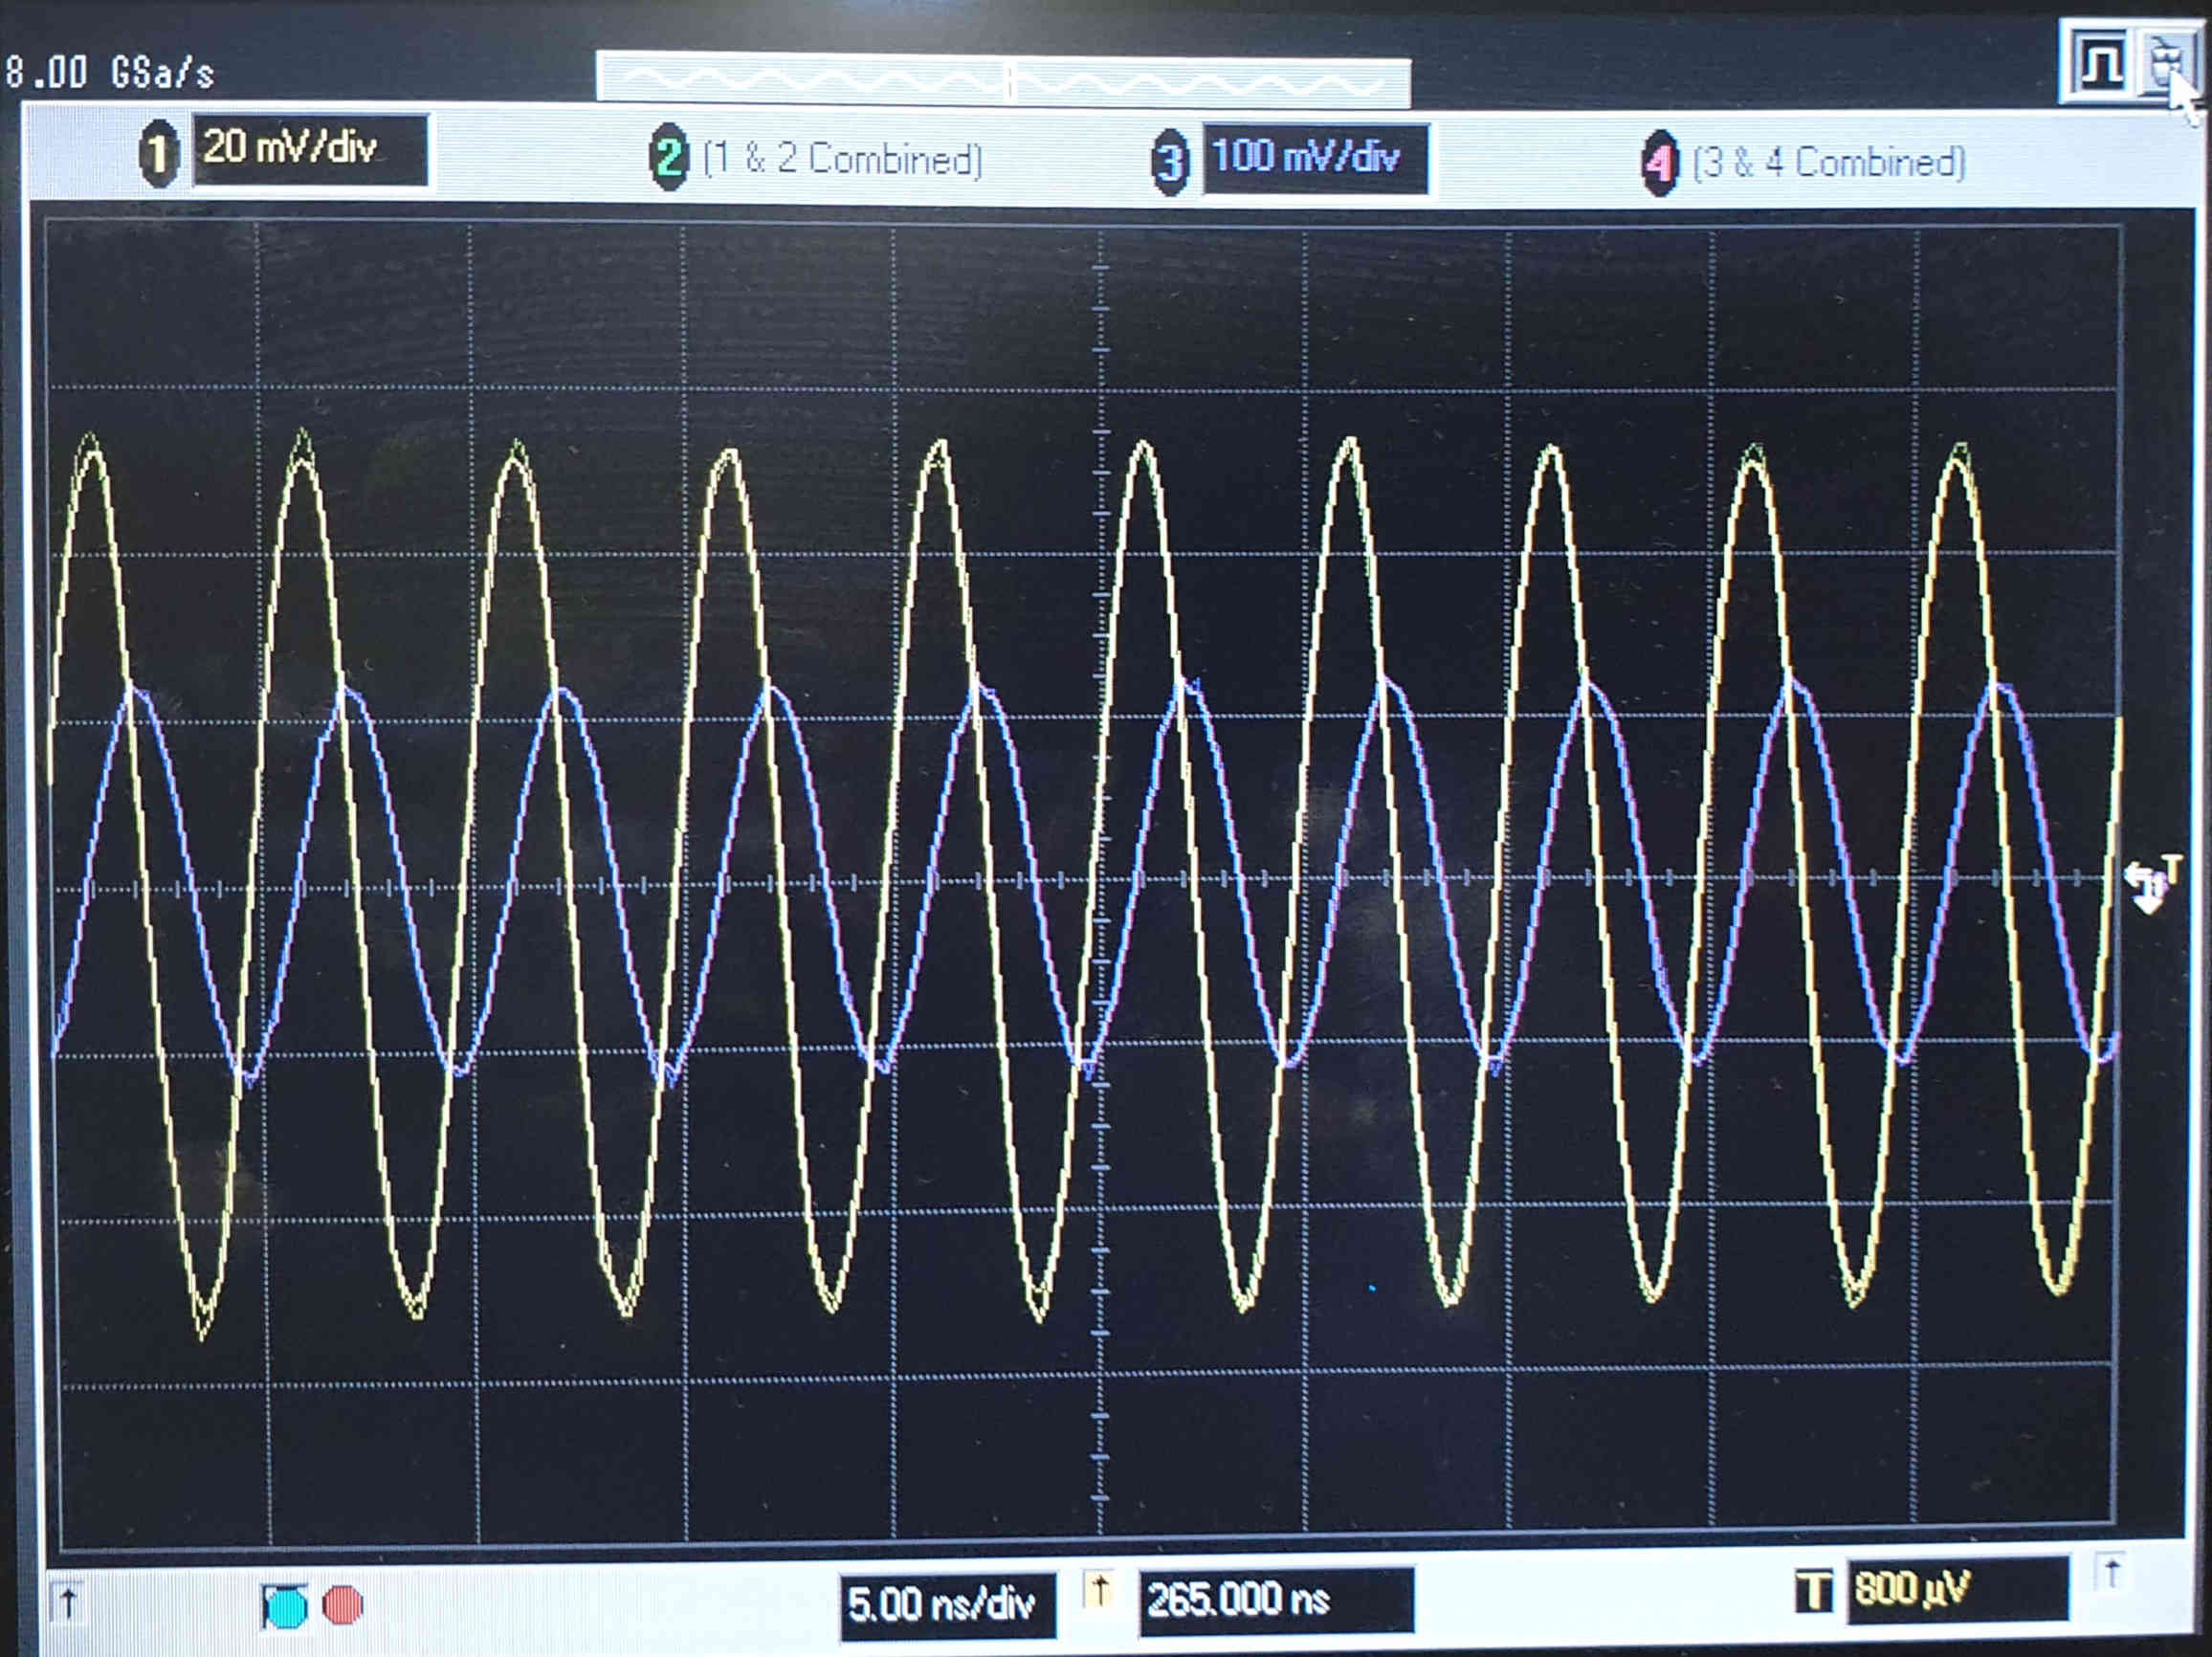
\includegraphics[width=\textwidth]{Bilder/Antenne_Phasenverschiebung1.jpg}
        \caption{parallele Ausrichtung beider Antennen}
    \end{subfigure}\hspace{1cm}
    \begin{subfigure}{0.45\textwidth}
        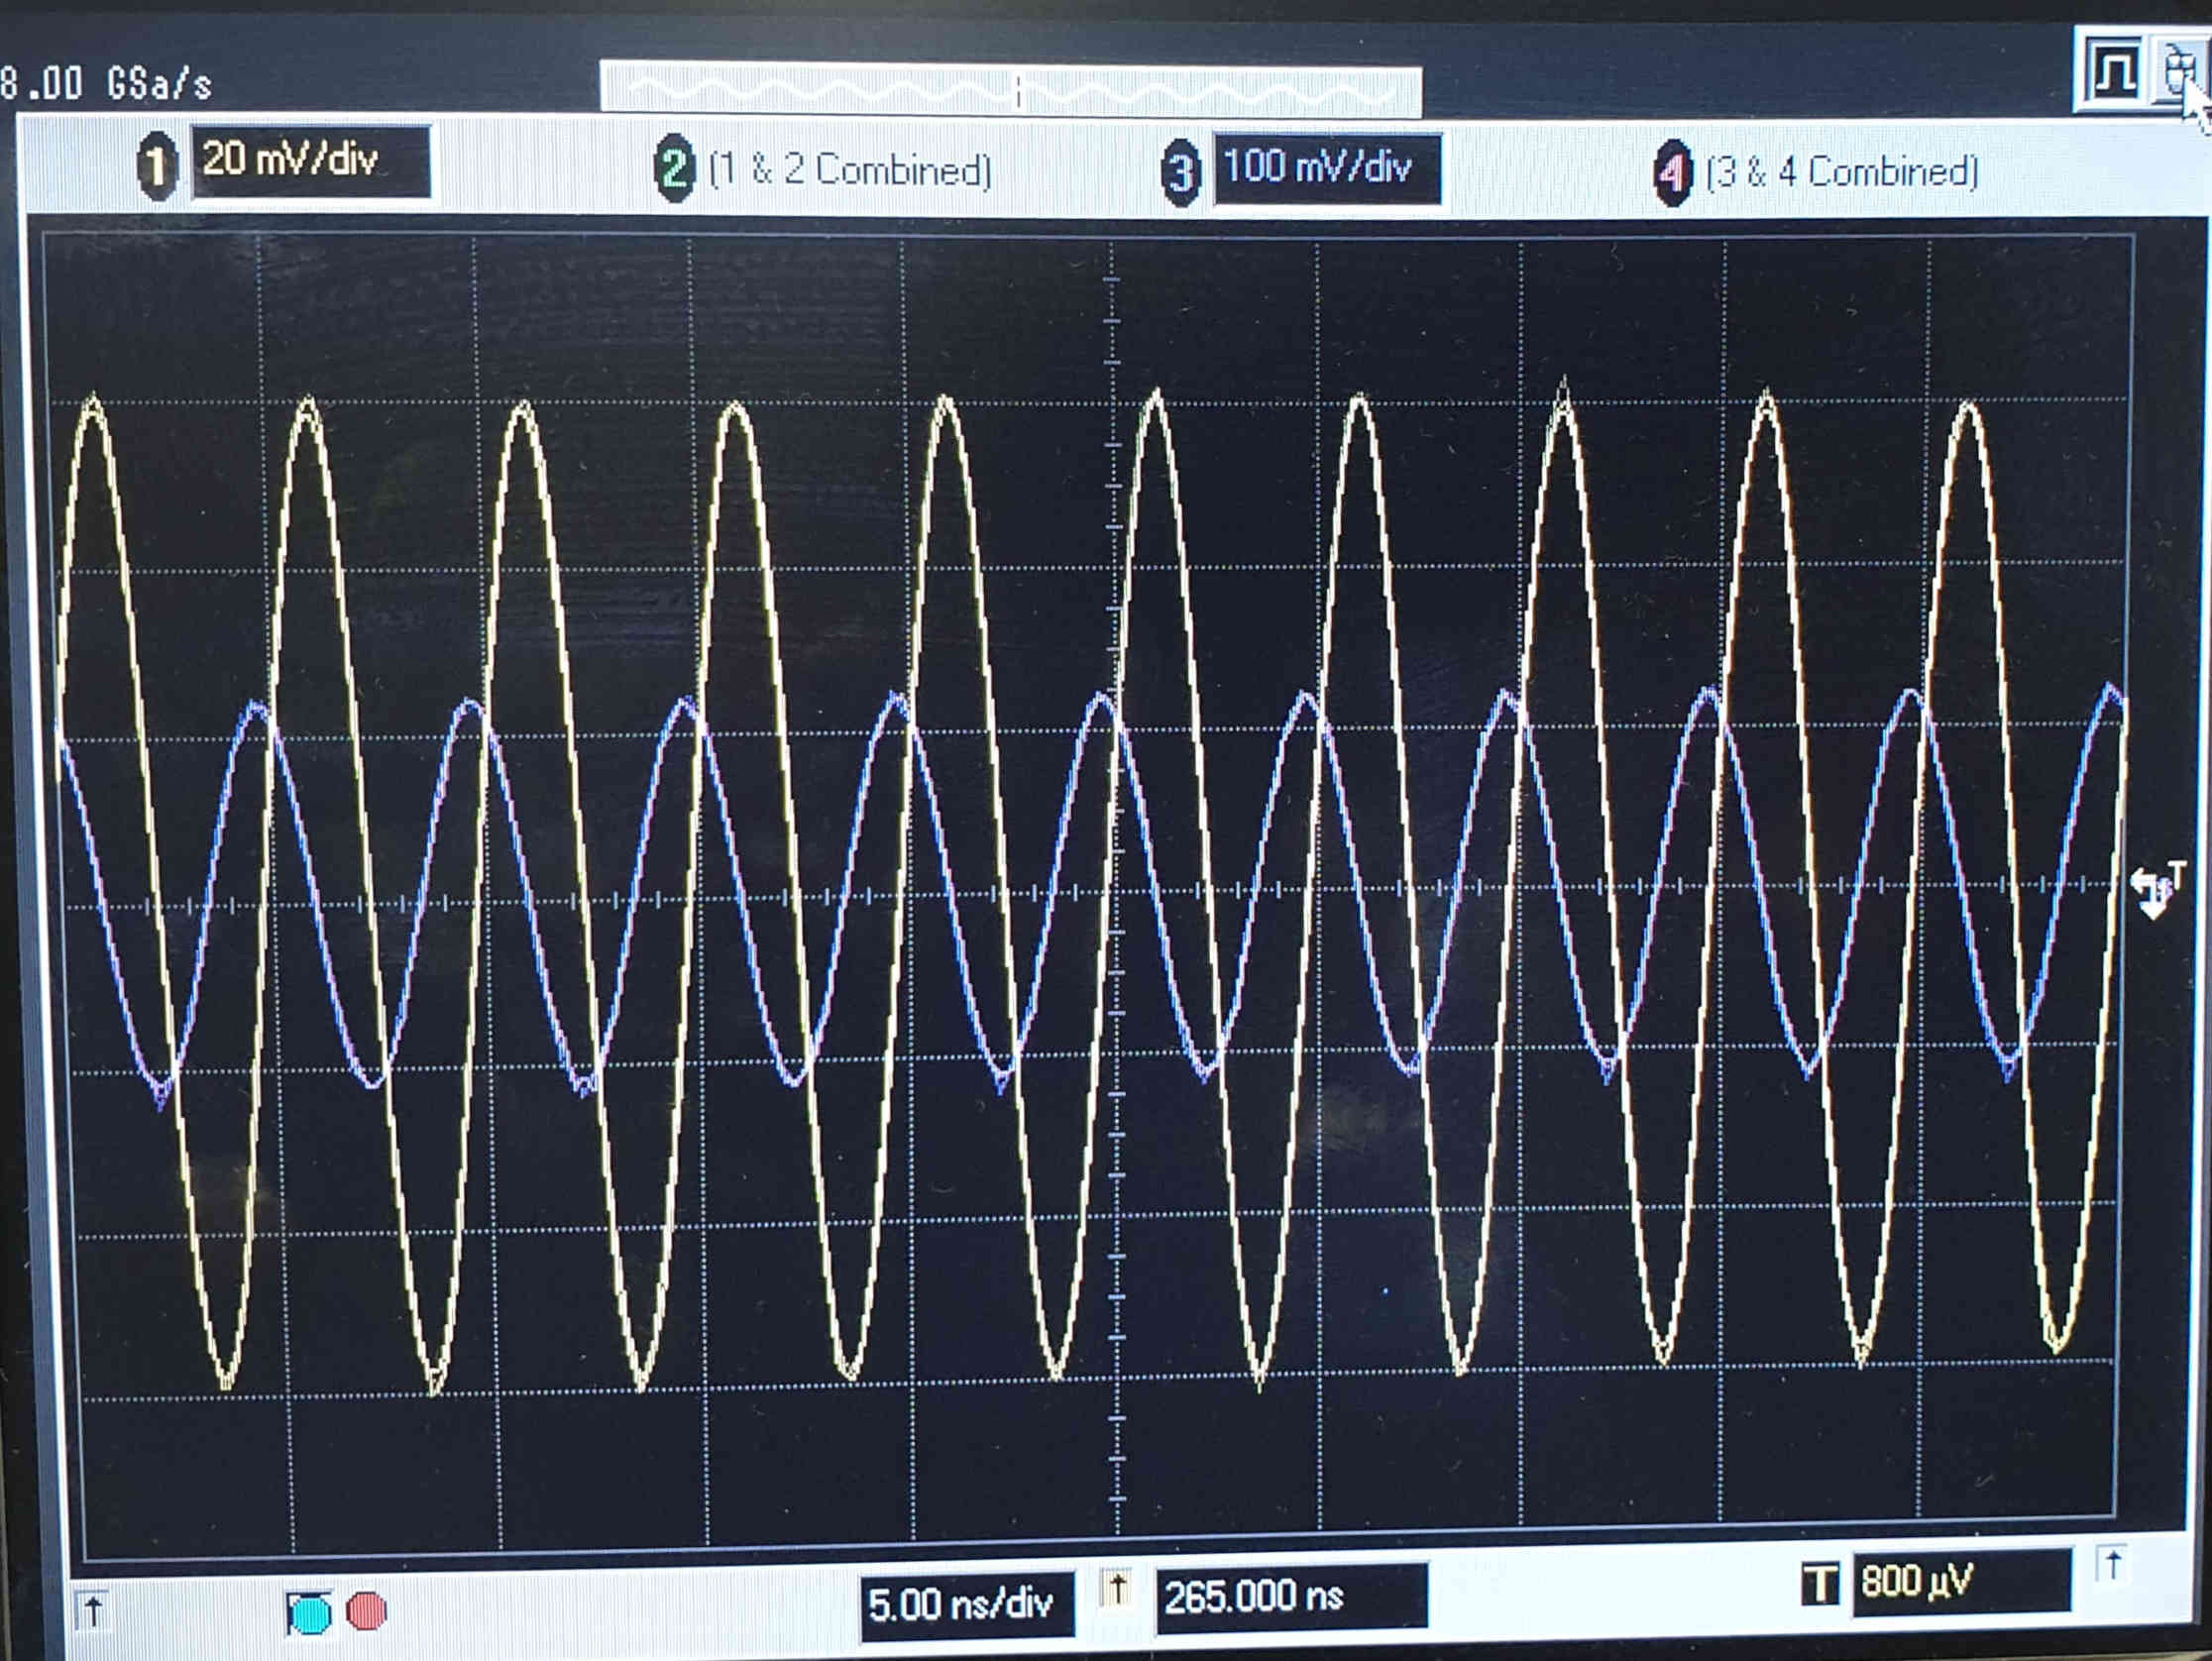
\includegraphics[width=\textwidth]{Bilder/Antenne_Phasenverschiebung2.jpg}
        \caption{parallele Ausrichtung beider Antennen, Drehen der Empfangsantenne um \SI{180}{\degree}}
    \end{subfigure}
    \caption{empfangenes (gelb) und gesendetes (blau) Signal bei unterschiedlicher Ausrichtung der Antennen zueinander}
\end{figure}

Beim Senden des modulierten Signals zeigt sich bei paralleler Ausrichtung beider Antennen und nachgeschalteter Demodulation am Zeitverlauf das ursprünglich gesendete Signal wieder. Werden beide Antennen annährend senkrecht zueinander gedreht, kommt das Signal zum Erliegen.

\begin{figure}[htp]
    \centering
    \begin{subfigure}{0.45\textwidth}
        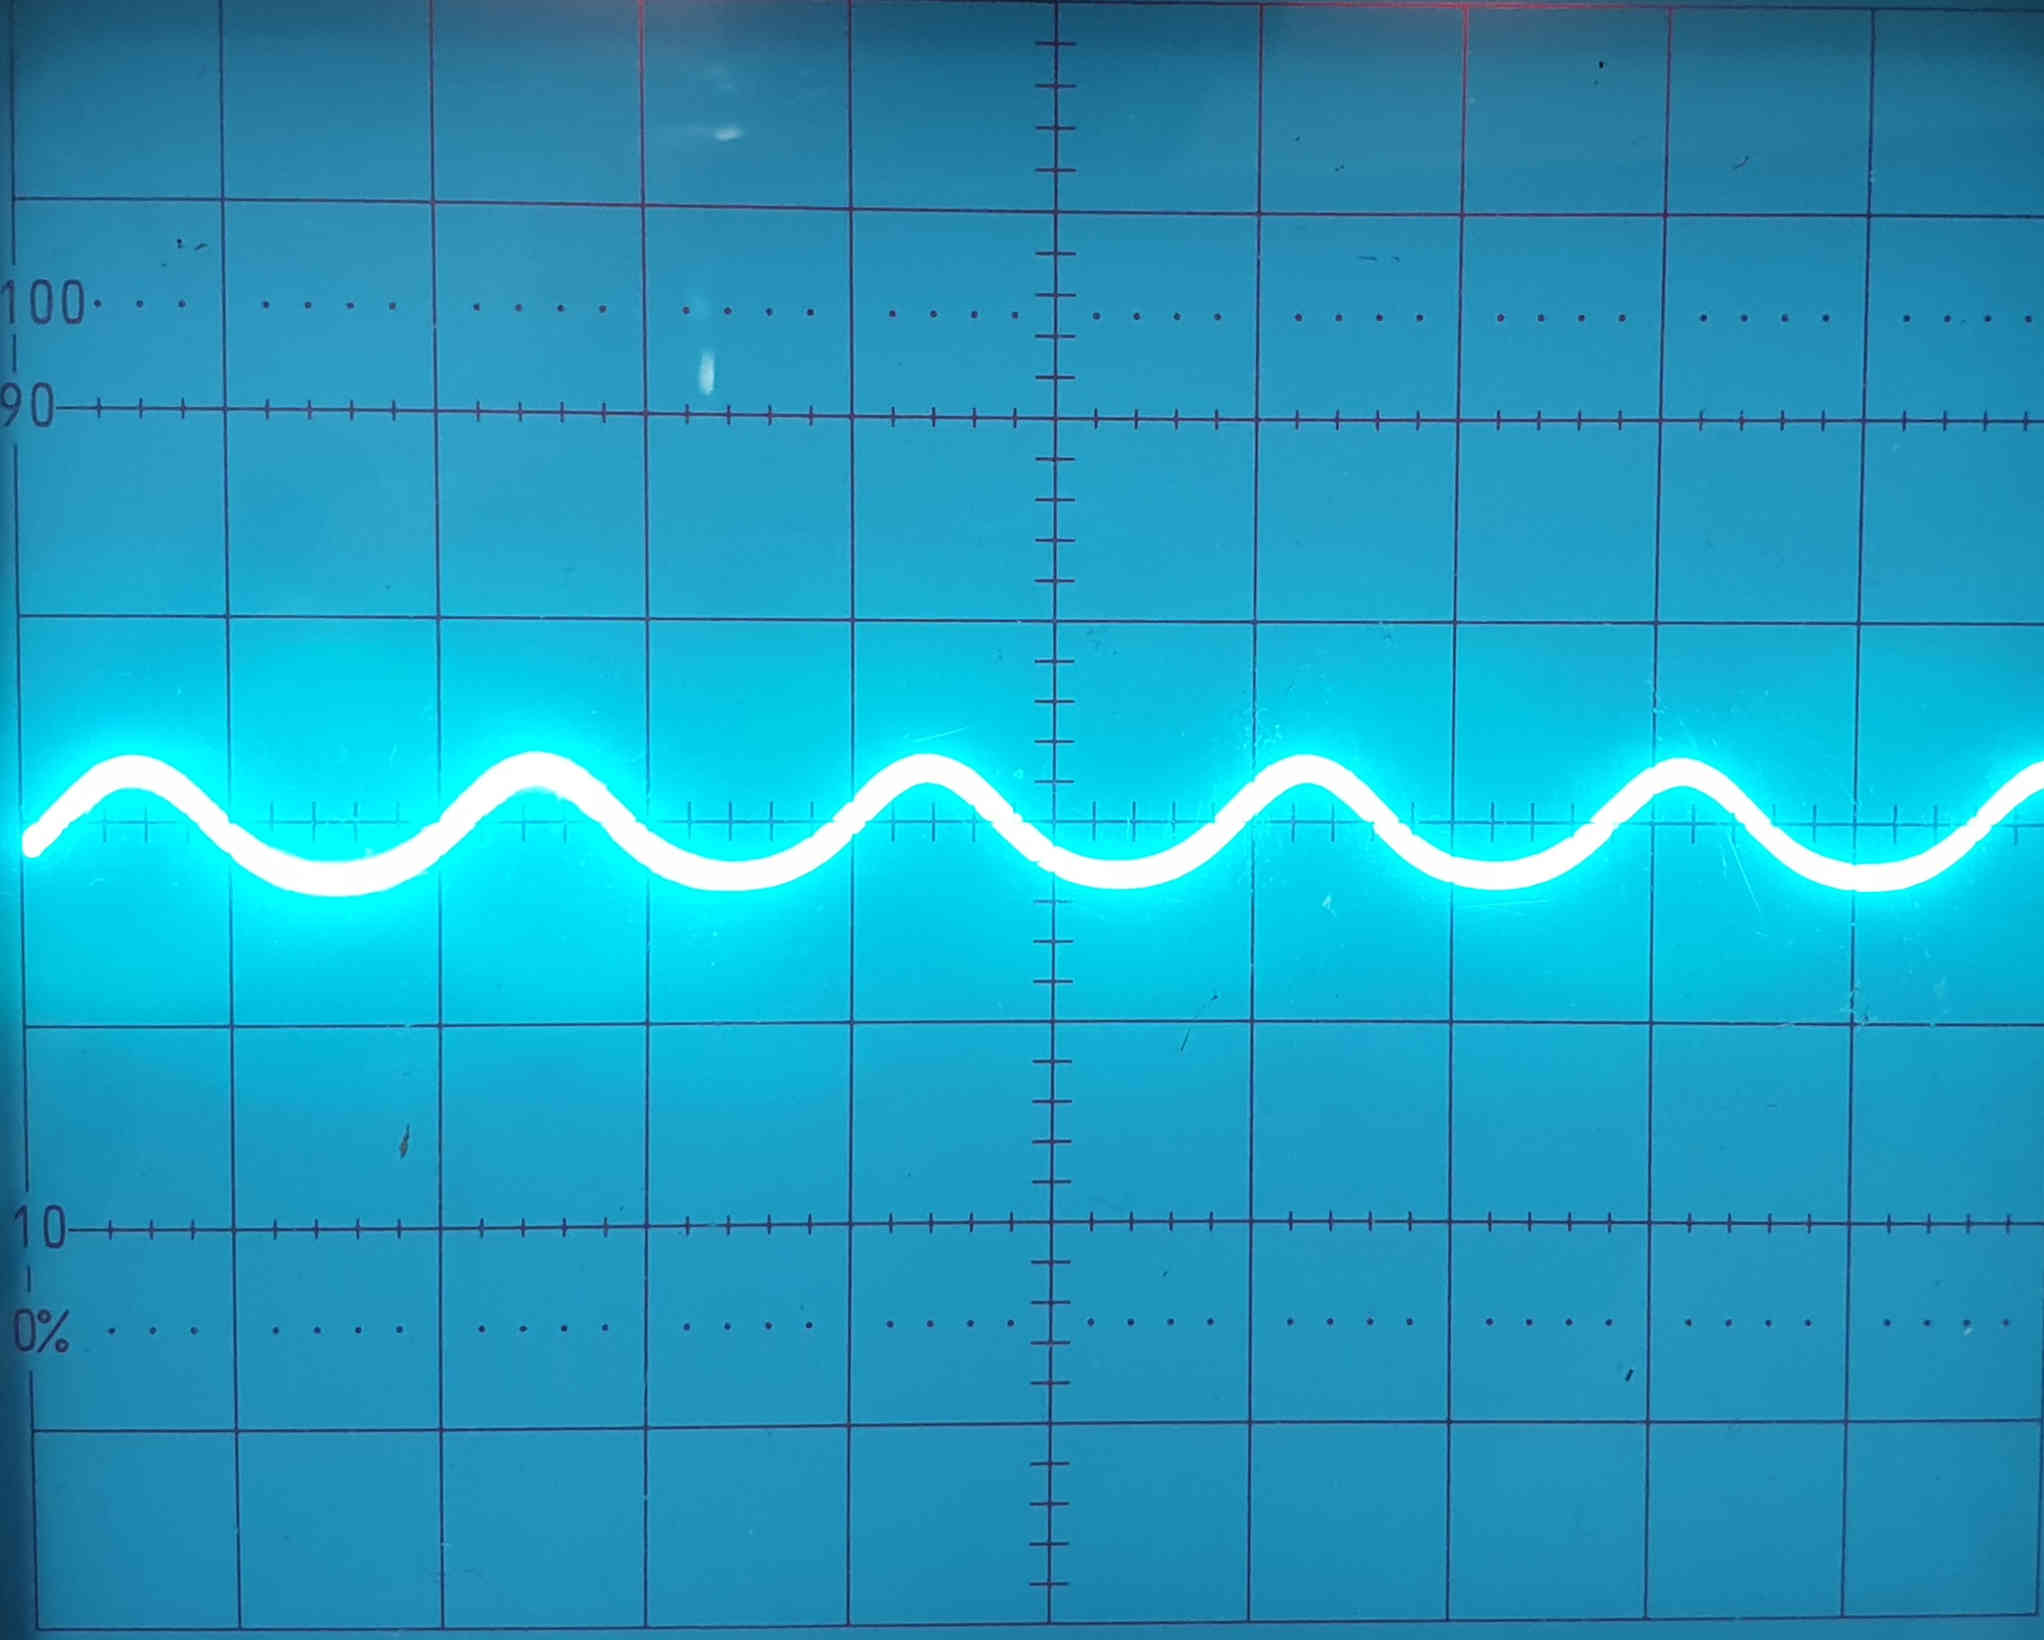
\includegraphics[width=\textwidth]{Bilder/Antenne_Demodulation_parallel.jpg}
        \caption{parallele Ausrichtung beider Antennen\\$~$}
    \end{subfigure}\hspace{1cm}
    \begin{subfigure}{0.45\textwidth}
        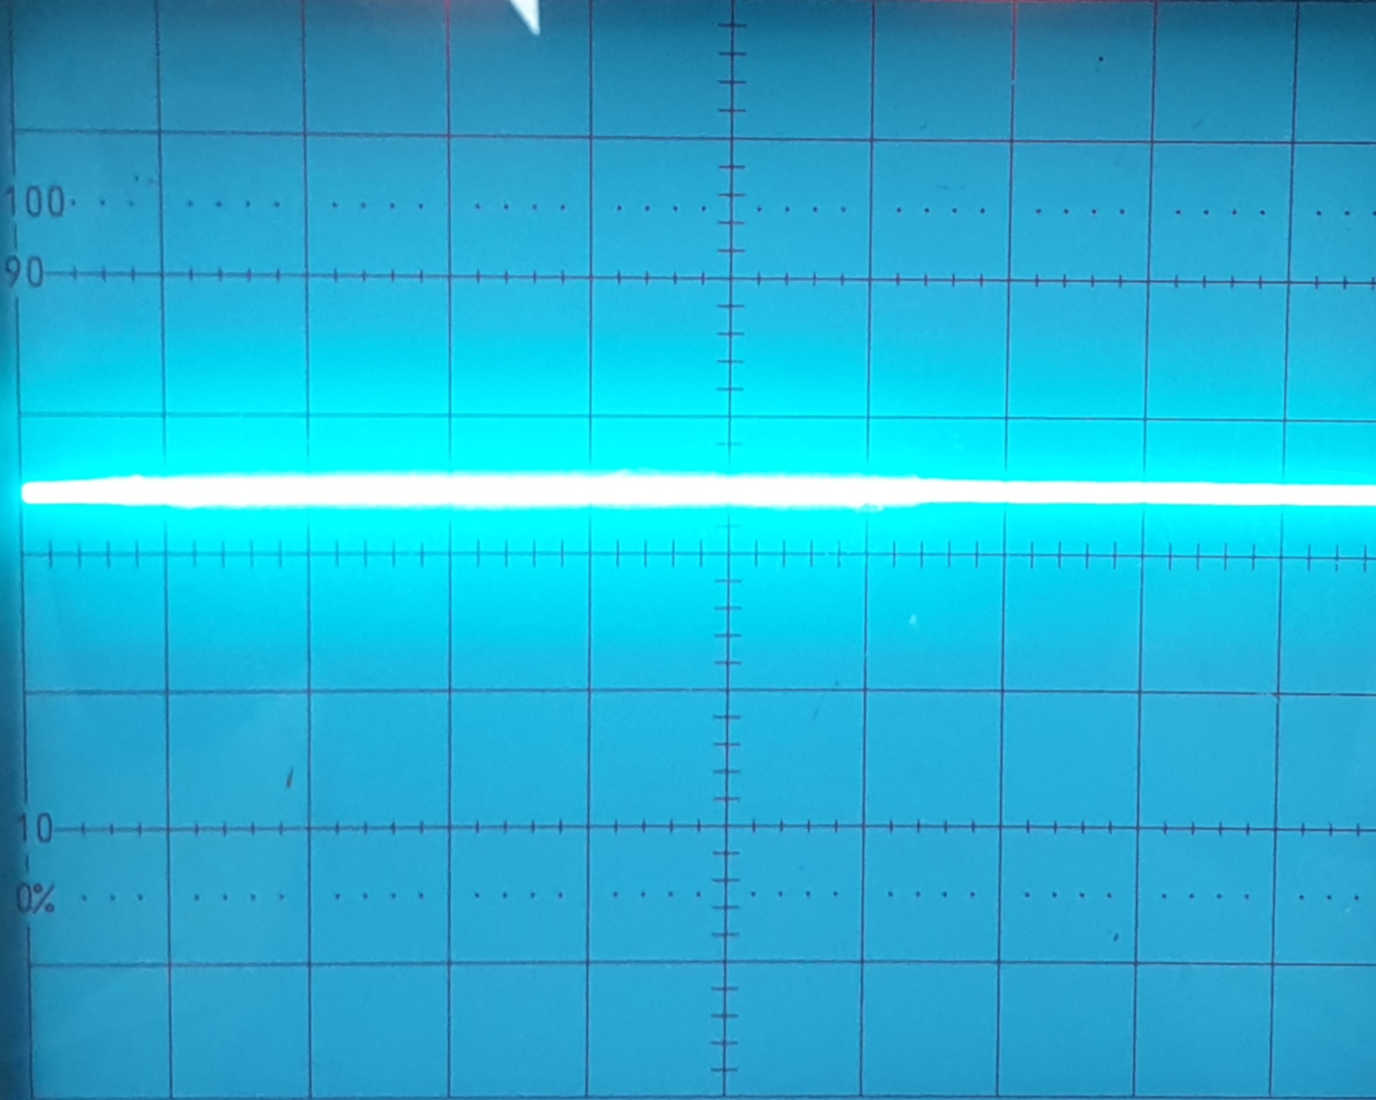
\includegraphics[width=\textwidth]{Bilder/Antenne_Demodulation_senkrecht.jpg}
        \caption{annähernd senkrechte Ausrichtung beider Antennen}
    \end{subfigure}
    \caption{empfangenes demoduliertes Signal bei unterschiedlicher Ausrichtung der Antennen zueinander}
\end{figure}

Außerdem wird das empfangene Signal hörbar gemacht. Dazu wird ein Lautsprecher anstelle des Spektrumanalysators angeschlossen. Beim Erhöhen der Amplitude der Nutzfrequenz wird der höhrbare Ton lauter. Wird die Frequenz der Nutzfrequenz erhöht, wird der Ton höher.
% *********************************************
% ***** KAPITEL 4 *****************************
% *********************************************
\section{Zusammenfassung}
Mithilfe der Untersuchung des Verhaltens von Sinussignalen auf verschiedenen Leitungen bei verschiedenen Anpassungen kann festgestellt werden, dass Laborkabel aufgrund ihres chaotischen Verhaltens bezüglich des Frequenzsgangs ungeeignet sind für die Übertragung von Hochfrequenzsignalen. Koaxialkabel bei einem Eingangswiderstand des Scopes von \SI{50}{\ohm} ermöglichen eine über alle Frequenzen gleiche Spannungsübertragung und verhindern das Ausbilden von Reflexionen. Die Fehlanpassung, die damit verbundene Ausbildung von Relfexionen und Verstärkung bzw Abschwächung der Spannung bei bestimmten Frequenzen kann jedoch auch bewusst genutzt werden. So kann ein Stichkabel mit offenem bzw. abgeschlossenem Ende verwendet werden, um dadurch einen Filter für bestimmte Frequenzen oder die Hochtransformation der Spannung bei bestimmten Frequenzen zu realisieren. \\
Bei der Untersuchung des Verhaltens von Rechtecksignalen auf Leitungen werden die unterschiedlichen Verhalten der Spannungen am Ende der Leitung bei unterschiedlichen Anpassungen bestätigt. Der Verlauf eines Signals durch die Leitung wird explizit deutlich. Außerdem wird festgestellt, dass dadurch die Ausbreitungsgeschwindigkeit, Verküzungsfaktor und Permitivität ermittelt werden können.\\ Zum Ende des ersten Versuchsteils werden zwei unterschiedliche Varianten zur Ermittlung des Wellenwiderstandes angewendet.\\
Da Signale niedriger Frequenz im freien Raum stark gedämpft werden, ist die Modulation der Nutzsignale auf Trägersignale hoher Frequenzen sinnvoll. Dabei wird das Signal per Amplituden- oder Frequenzmodulation in einen höheren Frequenzbereich verschoben. Der Empfänger gewinnt mithilfe eines Demodulators wieder das ursprüngliche Signal. Die Modulation liefert die Grundlage für die breiten Radiofrequenzbereich und verhindert, dass Programme auf gleichen Frequenzen gesendet werden, da bei der Modulation das Trägersignal beliebig wählbar ist.\\
Bei der Untersuchung der elektromagnetischen Wellen im freien Raum wird herausgefunden, dass nur ein Bruchteil der Sendeleistung auch wieder empfangen werden kann. Für das empfangene Signal ist die Orientierung der Sende- und Empfangsantennen von essentieller Bedeutung. Senkrechtes Ausrichten führt zu einem Auslöschen des Signals, während paralleles Ausrichten ein Maximum hervorruft, außerdem kann dadurch die Phasenverschiebung der Signale beeinflusst werden. Die Modulation wird als zentrales Element bei der Übertragung von Signalen bestätigt.

% ***** Literaturverzeichnis ******************

\begin{thebibliography}{xxx}
	\bibitem{Meinke}
	H. Meinke: \textit{Taschenbuch der Hochfrequenztechnik}. Springer Verlag Berlin Heidelberg New York 1992 (5. Auflage).
	\bibitem{Perner}
  I. Perner: \textit{FSU Fortgeschrittenenen Praktikum: Radiowellen}, Fried\-rich-Schil\-ler-Uni\-versi\-tät Juli 2019
  \bibitem{Amplitudenmodulation}
  Amplitudenmodulation: \url{https://de.wikipedia.org/wiki/Amplitudenmodulation}. Stand: 17.11.2019
  \bibitem{Leitungsgleichungen}
  Amplitudenmodulation: \url{https://de.wikipedia.org/wiki/Leitungsgleichung}. Stand: 01.12.2019
\end{thebibliography}

\end{document}
